% ------------------------------------------------------------------------
% ------------------------------------------------------------------------
% ICMC: Modelo de Trabalho Acadêmico (tese de doutorado, dissertação de
% mestrado e trabalhos monográficos em geral) em conformidade com 
% ABNT NBR 14724:2011: Informação e documentação - Trabalhos acadêmicos -
% Apresentação
% ------------------------------------------------------------------------
% ------------------------------------------------------------------------

% Opções: 
%   Qualificação          = qualificacao 
%   Curso                 = doutorado/mestrado
%   Situação do trabalho  = pre-defesa/pos-defesa (exceto para qualificação)
%   Versão para impressão = impressao
\documentclass[doutorado, pre-defesa]{packages/icmc}

% ---------------------------------------------------------------------------
% Pacotes Opcionais
% ---------------------------------------------------------------------------
\usepackage{rotating}           % Usado para rotacionar o texto
\usepackage[all,knot,arc,import,poly]{xy}   % Pacote para desenhos gráficos
% Este pacote pode conflitar com outros pacotes gráficos como o ``pictex''
% Então é necessário usar apenas um dos pacotes conflitantes
\newcommand{\VerbL}{0.52\textwidth}
\newcommand{\LatL}{0.42\textwidth}
% ---------------------------------------------------------------------------

% ---------------------------------------------------------------------------
% Pacotes e Comandos Adicionais (FalvoJr)
% ---------------------------------------------------------------------------
\usepackage{caption}
\usepackage{multirow}
\usepackage{fontawesome}

\newcolumntype{C}[1]{>{\centering}m{#1}}
\newcolumntype{P}[1]{>{\centering\arraybackslash}p{#1}}
\newcommand{\fullcite}[5]{%
  #1 \emph{#2}. \textbf{#3}. #4. #5.
}
% ---------------------------------------------------------------------------


% ---
% Informações de dados para CAPA e FOLHA DE ROSTO
% ---
% Tanto na capa quanto nas folhas de rosto apenas a primeira letra da primeira palavra (ou nomes próprios) devem estar em letra maiúscula, todas as demais devem ser em letra minúscula.
\tituloPT{Speech2Learning: Uma Arquitetura de Software Baseada em Reconhecimento de Fala Para Promover a Acessibilidade de Objetos de Aprendizagem}
\tituloEN{Speech2Learning: A Speech Recognition-Based Software Architecture to Promote the Accessibility of Learning Objects}
\autor[FalvoJr, V.]{Venilton FalvoJr}
\genero{M} % Gênero do autor (M = Masculino / F = Feminino)
\orientador[Orientadora]{Profa. Dra.}{Ellen Francine Barbosa}
%\coorientador{Prof. Dr.}{Fulano de Tal}
\curso{CCMC}
\data{13}{08}{2024} % Data do depósito
\idioma{PT} % Idioma principal do documento (PT = português / EN = inglês)
% ---


% ---
% RESUMOS
% ---

% Resumo em PORTUGUÊS
% conter no máximo 500 palavras
% conter no mínimo 1 e no máximo 5 palavras-chave
\textoresumo[brazil]{
    TODO. 
    }{TODO, TODO, TODO, TODO, TODO}


% resumo em INGLÊS
% conter no máximo 500 palavras
% conter no mínimo 1 e no máximo 5 palavras-chave
\textoresumo[english]{
    TODO. 
    }{TODO, TODO, TODO, TODO, TODO}


% ----------------------------------------------------------
% ELEMENTOS PRÉ-TEXTUAIS
% ----------------------------------------------------------

% Inserir a ficha catalográfica
\incluifichacatalografica{tex/pre-textual/ficha-catalografica.pdf}

% DEDICATÓRIA / AGRADECIMENTO / EPÍGRAFE
\textodedicatoria*{tex/pre-textual/dedicatoria}
\textoagradecimentos*{tex/pre-textual/agradecimentos}
\textoepigrafe*{tex/pre-textual/epigrafe}

% Inclui a lista de figuras
\incluilistadefiguras

% Inclui a lista de tabelas
\incluilistadetabelas

% Inclui a lista de quadros
%\incluilistadequadros

% Inclui a lista de algoritmos
%\incluilistadealgoritmos

% Inclui a lista de códigos
\incluilistadecodigos

% Inclui a lista de siglas e abreviaturas
\incluilistadesiglas

% Inclui a lista de símbolos
\incluilistadesimbolos

% ----
% Início do documento
% ----
\begin{document}
% ----------------------------------------------------------
% ELEMENTOS TEXTUAIS
% ----------------------------------------------------------
\textual

\chapter{Introdução}
\label{chapter1}
\section{Contexto e Motivação}

A acessibilidade digital é um componente essencial para a inclusão social, especialmente no contexto educacional, onde a variedade de perfis e necessidades dos alunos demanda soluções genuinamente inclusivas. Segundo dados do \sigla{IBGE}{Instituto Brasileiro de Geografia e Estatística}, no Brasil, aproximadamente 8,9\% da população com mais de 2 anos, o que corresponde a 18,6 milhões de pessoas, possui algum tipo de deficiência \cite{IBGE2023}.

Nesse cenário, a área do conhecimento de \sigla{TA}{Tecnologia Assistiva} se apresenta como uma resposta natural. De acordo com \citeonline{Cook2020}, soluções de TA englobam uma ampla gama de recursos, desde dispositivos e serviços até práticas voltadas para melhorar as capacidades funcionais e a qualidade de vida das \sigla{PcD}{Pessoas com Deficiência}. A TA é uma área interdisciplinar que combina produtos, metodologias e estratégias, todas direcionadas a aumentar a autonomia e a participação das PcD em suas atividades cotidianas \cite{Cat2009}.

Além disso, o \sigla{CAT}{Comitê de Ajudas Técnicas} do Brasil destaca que a TA desempenha um papel essencial na promoção da autonomia, independência e inclusão social dessas pessoas. As soluções de TA vão além de artefatos tecnológicos, abrangendo também serviços e práticas adaptadas às necessidades específicas dos usuários em diferentes contextos \cite{Cat2009}. Dessa forma, a TA tem o potencial de ampliar o acesso a recursos educacionais, considerando as particularidades de cada aprendiz \cite{UNESCO2023, GovBr2023}.

O uso de \sigla{TICs}{Tecnologias de Informação e Comunicação}, que podem incluir recursos e serviços de TA, desempenha um papel essencial nesse contexto. Os relatórios da \citeonline{OMS2011, OMS2018} enfatizam que a promoção da acessibilidade digital por meio das TICs é vital para garantir a participação plena de todas as pessoas na sociedade e proporcionar oportunidades igualitárias de desenvolvimento educacional e profissional.

Ainda no âmbito das TICs, as \sigla{IAs}{Inteligências Artificiais} surgem como ferramentas poderosas para promover a acessibilidade. A \sigla{UNESCO}{Organização das Nações Unidas para a Educação, a Ciência e a Cultura} destaca o potencial transformador das TICs na educação e ressalta a importância do \textit{Design} Universal na criação de soluções acessíveis a todos, independentemente de suas habilidades ou deficiências \cite{UNESCO2023, GovBr2023}. Nesse contexto, as IAs podem revolucionar a educação, fornecendo ferramentas que democratizam o acesso ao conhecimento e aprimoram a experiência de aprendizagem para todos os estudantes \cite{Holmes2019,UNESCO2024}.

No entanto, apesar do potencial das TICs e IAs na área do conhecimento de TA, o Brasil ainda enfrenta muitos desafios para a inclusão de PcD no ambiente educacional. Dados de 2022 indicam que 19,5\% das PcD estão fora da escola, uma taxa significativamente maior em comparação aos 4,1\% entre pessoas sem deficiência \cite{IBGE2023}. Essa disparidade é frequentemente agravada pela falta de recursos de TA, destacando a necessidade de investimentos em soluções que ampliem o acesso e a permanência de PcD em ambientes educacionais inclusivos.

Sob esse olhar, neste trabalho de doutorado é proposta a \textit{Speech2Learning}, uma arquitetura de software baseada em \sigla{ASR}{\textit{Automatic Speech Recognition}}, com o objetivo de promover a criação de \sigla{OAs}{Objetos de Aprendizagem} mais acessíveis utilizando reconhecimento de fala. Segundo \citeonline{Wiley2000}, OAs são recursos digitais reutilizáveis projetados para apoiar o processo de ensino-aprendizagem. Já o ASR, também conhecido como \sigla{STT}{\textit{Speech-to-Text}}, é uma subárea da IA que converte fala em texto \cite{Jurafsky2024}, possibilitando a acessibilidade em OAs audíveis, como videoaulas. A integração desses conceitos na \textit{Speech2Learning} não apenas beneficia PcD, mas qualquer aprendiz que possa se beneficiar do uso de legendas ou transcrições automáticas.

A motivação para este trabalho de doutorado emerge das lacunas identificadas durante um \sigla{MS}{Mapeamento Sistemático} que investigou estudos sobre línguas de sinais e TICs \cite{FalvoJr2020_FIE, FalvoJr2020_SBIE, FalvoJr2021_RENOTE}. Este estudo revelou uma carência significativa de soluções padronizadas e reutilizáveis para promover a acessibilidade em diversos contextos educacionais. Com o advento das IAs, especialmente em modelos de reconhecimento de fala, surgiu a oportunidade de projetar uma arquitetura de software que atendesse a essas demandas.

A \textit{Speech2Learning} é concebida como uma resposta a esse cenário, utilizando o ASR para transcender barreiras no acesso à informação e expandir a acessibilidade de OAs audíveis, atendendo a um público de aprendizes mais amplo. Ao longo deste trabalho, foram criadas duas instâncias concretas da \textit{Speech2Learning}, as quais permitiram avaliar a arquitetura por meio de estudos de caso aplicados na indústria. Essas instâncias, além de servirem como avaliação prática da arquitetura, se estabelecem como recursos de TA ao expandirem o alcance dos OAs audíveis, contribuindo para um processo de ensino-aprendizagem mais acessível.

\section{Objetivos e Questões da Pesquisa}

O principal objetivo deste trabalho de doutorado é desenvolver e avaliar uma arquitetura de software que apoie a expansão da acessibilidade de objetos de aprendizagem audíveis, promovendo o desenvolvimento de recursos e serviços de TA. Para alcançar este objetivo, foram definidas as seguintes questões de pesquisa:

\begin{itemize}
    \item \textbf{QP1:} Como uma arquitetura de software voltada para a acessibilidade de Objetos de Aprendizagem (OAs) audíveis pode ser desenvolvida para apoiar a inclusão educacional de diferentes grupos de usuários, promovendo maior igualdade de acesso à educação em diversos contextos?
    
    \begin{itemize}
        \item \textbf{QP1.1:} De que maneira as tecnologias de Reconhecimento Automático de Fala (ASR) podem contribuir para melhorar a acessibilidade educacional?
        
        \begin{itemize}
            \item \textbf{Questão Avaliativa:} Qual é o nível de precisão dos serviços de ASR, oferecidos pelos principais provedores do mundo, nos processos de transcrição e legendagem de videoaulas?
        \end{itemize}
        
        \item \textbf{QP1.2:} Como as tecnologias de ASR podem ser adaptadas para atender às necessidades de acessibilidade de usuários da Libras?
        
        \begin{itemize}
            \item \textbf{Questão Avaliativa:} Qual é a percepção dos intérpretes de Libras em relação à precisão dos avatares de línguas de sinais baseados em texto, integrados às transcrições automáticas em um \textit{player} de vídeo com \textit{Design} Universal?
        \end{itemize}
    
    \end{itemize}

\end{itemize}

\subsection*{Objetivos Específicos:}

\begin{enumerate}
\item Investigar e identificar os requisitos fundamentais para a proposição de uma arquitetura de software voltada para a acessibilidade de OAs audíveis, considerando diferentes contextos educacionais e grupos de usuários.
\item Desenvolver \sigla{POCs}{Provas de Conceito} na indústria, visando aferir a viabilidade prática da arquitetura de software. Dentre as POCs, incluem-se:
\begin{itemize}
\item Uma API para a transcrição e legendagem automática de videoaulas, com uma interface padronizada e de fácil integração a diferentes aplicações educacionais.
\item Um \textit{player} de vídeo baseado nos princípios do \textit{Design} Universal, capaz de integrar avatares de Libras baseados em texto, conectados às transcrições automáticas.
\end{itemize}
\item Avaliar as soluções desenvolvidas como POCs, incluindo as transcrições/legendas automáticas e a integração com avatares de Libras, por meio de estudos de caso que utilizem métodos quantitativos e qualitativos.
\item Discutir o potencial de replicação e adaptação das soluções desenvolvidas para diferentes contextos educacionais, destacando a flexibilidade e aplicabilidade da arquitetura proposta para promover inclusão e acessibilidade.
\end{enumerate}

\section{Percurso Metodológico}

A proposta da \textit{Speech2Learning} foi consolidada após um MS focado em estudos sobre línguas de sinais e TICs, que evidenciou uma carência de soluções padronizadas e reutilizáveis em múltiplos contextos educacionais. Este estudo revelou uma oportunidade para o desenvolvimento de uma arquitetura de software que transcendesse as limitações específicas das línguas de sinais, promovendo uma estrutura genérica voltada para o desenvolvimento de recursos e/ou serviços de TA baseados em ASR, com o intuito de tornar os OAs audíveis mais acessíveis \cite{FalvoJr2020_FIE, FalvoJr2020_SBIE, FalvoJr2021_RENOTE}.

Dentro desse contexto, a Arquitetura \textit{Speech2Learning} foi concebida como uma diretriz de software robusta e flexível, voltada para a transcrição automática e a geração de legendas de conteúdos educacionais, com o objetivo de melhorar a acessibilidade de OAs. A arquitetura foi avaliada por meio de dois estudos de caso realizados em parceria com a \textit{EdTech} brasileira DIO (\url{https://dio.me}). A DIO é uma plataforma de ensino com mais de 1 milhão de usuários, dedicada a capacitar profissionais em tecnologia, conectando-os com as empresas mais inovadoras do mundo por meio de uma metodologia educacional com foco em empregabilidade. 

Essa colaboração proporcionou acesso aos OAs e à infraestrutura necessários para implementar e avaliar as soluções propostas, que foram previamente validadas por meio de POCs conduzidas dentro da própria \textit{EdTech}. A seguir, os detalhes dos estudos de caso:

\begin{itemize}
\item \textbf{\textit{Estudo de Caso 1 -- Legendas Automáticas de Videoaulas}}: Implementação de uma API para a transcrição e legendagem de videoaulas. Essa API, desenvolvida conforme as diretrizes da \textit{Speech2Learning}, integrou serviços de ASR baseados em IA oferecidos por empresas líderes do setor, segundo o \citeonline{Gartner2023}: Amazon, Google, IBM, Microsoft e OpenAI, essa última devido ao seu destaque em soluções extremamente difundidas atualmente, como o ChatGPT. 

A precisão e qualidade das transcrições automáticas fornecidas por cada provedor foram avaliadas utilizando algoritmos de similaridade léxica e um \textit{Survey} que capturou as percepções dos usuários sobre a acurácia das legendas geradas. A combinação desses dados quantitativos com uma análise documental, que forneceu uma perspectiva qualitativa, foi essencial para uma abordagem de triangulação de dados, possibilitando uma avaliação abrangente das transcrições automáticas a partir de múltiplas perspectivas \cite{FalvoJr2023_HICSS, FalvoJr2024_FIE}.

\item \textbf{\textit{Estudo de Caso 2 -- Player de Vídeo com Avatar de Libras}}: Desenvolvimento de um \textit{player} de vídeo aderente ao conceito de \textit{Design} Universal \cite{GovBr2023}, projetado para a integração com avatares de línguas de sinais, como a Libras. A \sigla{Libras}{Língua Brasileira de Sinais} é uma língua gestual utilizada pela comunidade surda no Brasil, reconhecida legalmente desde 2002 \cite{Quadros2017, Quadros2019, Honora2021}. Nesta segunda instância da \textit{Speech2Learning}, o ASR foi combinado com avatares de Libras baseados em texto, demonstrando a sinergia dessas soluções de TA para tornar os OAs mais acessíveis. 

O potencial desta solução foi avaliado por meio de um \textit{Survey} e de entrevistas com intérpretes de Libras. Esses métodos permitiram a coleta de dados quantitativos, como a avaliação dos intérpretes sobre a qualidade das sinalizações dos avatares, e de dados qualitativos, que forneceram percepções detalhadas sobre a relevância do \textit{Player} de Vídeo em contextos educacionais para usuários da Libras. Assim, o estudo possibilitou uma análise interessante sobre a eficácia dos melhores avatares de Libras quando aplicados a videoaulas transcritas automaticamente.
\end{itemize}

A condução de estudos de caso, conforme definido por \citeonline{Sommerville2015, Pressman2016}, mostrou-se apropriada neste contexto, pois permitiu uma análise detalhada e contextualizada da aplicação prática da arquitetura \textit{Speech2Learning} em situações reais na \textit{EdTech} DIO. Essa abordagem proporcionou uma compreensão aprofundada dos impactos, desafios e potencialidades da arquitetura na implementação de soluções acessíveis, oferecendo percepções valiosas para o desenvolvimento de TA adaptável a diversos contextos educacionais.

Este trabalho, portanto, não apenas aborda um problema social relevante, mas também contribui para o campo da acessibilidade digital, fornecendo uma base sólida para o desenvolvimento de soluções em TA adaptáveis a diferentes contextos educacionais. Através da Arquitetura \textit{Speech2Learning} e de suas instâncias implementadas, espera-se promover um impacto significativo na acessibilidade educacional, abrindo novos caminhos para a inclusão e a igualdade no acesso aos OAs.

\section{Organização}

Esta tese está organizada em cinco capítulos, além das referências e apêndices. Após a introdução, que contextualiza a pesquisa e define os objetivos, a fundamentação teórica é explorada no \autoref{chapter2}, discutindo os principais conceitos e trabalhos relacionados ao tema de pesquisa. O \autoref{chapter3} detalha a Arquitetura \textit{Speech2Learning}, apresentando desde sua concepção até suas camadas e respectivas responsabilidades para promover OAs mais acessíveis. O \autoref{chapter4} apresenta a aplicação prática da Arquitetura \textit{Speech2Learning} em dois estudos de caso, demonstrando suas possibilidades de implementação. Por fim, o \autoref{chapter5} consolida as conclusões e expande algumas discussões com foco em \textit{insights} para trabalhos futuros.

\chapter{Fundamentação Teórica}
\label{chapter2}
\section{Considerações Iniciais}

A fundamentação teórica deste estudo começa com um \sigla{MS}{Mapeamento Sistemático}, cujo objetivo é identificar a interseção entre as TICs e as línguas de sinais no contexto educacional. A \autoref{section:foundation:sm} oferece um resumo deste MS, enquanto análises mais detalhadas dos estudos primários, que abrangem tanto o panorama nacional quanto internacional, estão disponíveis em nossas publicações anteriores: \citeonline{FalvoJr2020_FIE, FalvoJr2020_SBIE, FalvoJr2021_RENOTE}.

A realização deste estudo permitiu identificar \textit{gaps} tecnológicos no uso de línguas de sinais no ensino-aprendizagem, destacando a necessidade de novas pesquisas na literatura. Complementar ao MS, um levantamento bibliográfico complementar foi conduzido para explorar conceitos e TICs promissoras que possam enfrentar esses desafios. As seções subsequentes expandem essas temáticas, abordando Arquiteturas de Software (\autoref{section:foundation:arch}), OAs (\autoref{section:foundation:lo}) e ASR (\autoref{section:foundation:asr}). Fornecendo assim, a base teórica para a \textit{Speech2Learning}, uma arquitetura baseada em ASR para OAs audíveis mais acessíveis, definida em detalhes no \autoref{chapter3}.

\section{Mapeamento Sistemático: TICs e Línguas de Sinais na Educação}
\label{section:foundation:sm}

Para definir o escopo deste projeto, foi crucial realizar um estudo sistemático de literatura para identificar lacunas e oportunidades tecnológicas no processo de ensino e aprendizagem com línguas de sinais. De acordo com \citeonline{Kitchenham2007}, existem duas abordagens principais para este tipo de estudo: revisão ou mapeamento sistemáticos. Optou-se pelo MS devido à sua capacidade de apresentar evidências de um domínio de estudo em um alto nível de granularidade, agrupando-as em áreas de similaridade e identificando tendências emergentes.

O protocolo de pesquisa para o MS foi cuidadosamente definido com base em diretrizes formais  \cite{Kitchenham2007, Nakagawa2010, Zhang2011, Petersen2015}. A abordagem de \citeonline{Zhang2011} foi particularmente relevante, pois orientou a estratégia de busca e os critérios de qualidade adotados no estudo. Essa estratégia foi adaptada para aumentar o rigor do processo de pesquisa, incorporando o \sigla{QGS}{\textit{Quasi-Gold Standard}} e seguindo boas práticas recomendadas na literatura (\autoref{ms:zhang-approach}).

\begin{figure}[htb]
\centering 
\caption{Busca Sistemática Baseada em QGS.}
\label{ms:zhang-approach}
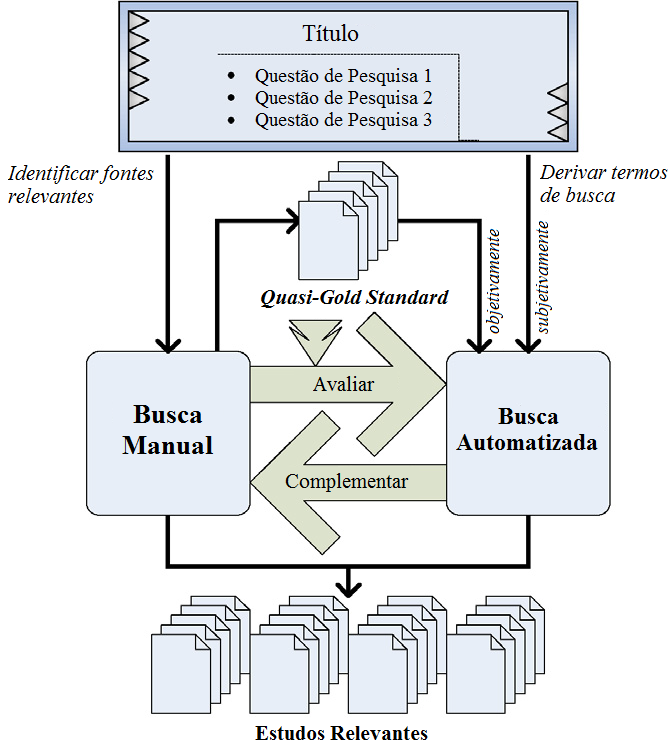
\includegraphics[width=0.675\textwidth]{images/chapter2-sm-zhang-approach.png}
\fadaptada{Zhang2011}
\end{figure}

\subsection{Definição do Escopo e Critérios de Seleção}
\label{ms:conducao-escopo}

As \sigla{QP}{Questões de Pesquisa} são essenciais para definir o escopo e identificar possíveis palavras-chave em um estudo sistemático de literatura \cite{Kitchenham2007,Petersen2015}. Neste contexto, uma abordagem comum se dá através da aplicação dos critérios de PICO \cite{Petticrew2008}. A \autoref{table:pico} representa o PICO, que derivaram as seguintes QP que definem o escopo deste MS.

\begin{table}[htb]
\centering
\caption{Critérios de PICO.}
\label{table:pico}
\begin{tabularx}{\textwidth}{lX} \hline
\textit{\textbf{P}opulation} & Aprendizes/Educadores interessados em línguas de sinais. \\
\textit{\textbf{I}ntervention} & TICs relevantes no processo de ensino-aprendizagem com línguas de sinais. \\
\textit{\textbf{C}omparison} & Não se aplica. \\
\textit{\textbf{O}utcome} & Panorama tecnológico sobre o ensino-aprendizagem com línguas de sinais. \\ \hline
\end{tabularx}
\end{table}

\begin{itemize}
    \setlength\itemsep{0em}
    \item \textbf{QP1}: Quais soluções tecnológicas vêm sendo propostas no processo de ensino-aprendizagem com línguas de sinais?
    % \begin{itemize}
    %     \item Quais são os tipos de soluções propostas (software ou hardware ou teóricas)?
    %     \item Quais tecnologias foram usadas?
    %     \item Quais métodos de avaliação foram aplicados?
    % \end{itemize}
    \item \textbf{QP2}: Quais tópicos educacionais são abordados?
    \item \textbf{QP3}: Quais línguas de sinais são abordadas?
    % \begin{itemize}
    %     \item Quais estudos abordam múltiplas línguas de sinais?
    % \end{itemize}
\end{itemize}

Segundo \citeonline{Kitchenham2007,Petersen2015}, os estudos sistemáticos requerem critérios explícitos de inclusão e exclusão para avaliar seus potenciais estudos primários. Assim, foram definimos os seguintes critérios de seleção:

\begin{table}[htb]
\centering
\caption{Critérios de Inclusão (CI) e Exclusão (CE).}
\label{tab:ms:criterios-selecao}
\begin{tabularx}{\textwidth}{lX} \hline
\textbf{CI1} & Os estudos apresentam contribuições (software ou hardware ou teóricas) para o ensino e a aprendizagem de línguas de sinais. \\ \hline
\textbf{CE1} & Estudos que não foram publicados no período de 2000 a 2019, seguindo um racional semelhante à \citeonline{Radermacher2013,Scatalon2019}, os quais sugerem que estudos anteriores a 2000 não representam as abordagens educacionais atuais, especialmente considerando o contexto de tecnologia. \\ \hline
\textbf{CE2} & Estudos classificados como resumos, resumos de conferências/editoriais, literatura cinza ou capítulos de livros. \\ \hline
\textbf{CE3} & Estudos não apresentados em inglês ou português. \\ \hline
\textbf{CE4} & Estudos não acessíveis em texto completo. \\ \hline
\textbf{CE5} & Estudos duplicados ou superficialmente complementares de outros estudos. \\ \bottomrule
\end{tabularx}
\end{table}

\subsection{Condução das Buscas Manual e Automatizada}
\label{ms:conducao-busca-manual}

No contexto das buscas manuais, a \autoref{ms:table:busca-manual-nacional} lista as conferências e periódicos nacionais analisados. No entanto, os estudos dessas fontes não foram incluídos na composição do QGS devido à limitação de indexação nos mecanismos de busca internacionais, o que poderia comprometer a eficácia da abordagem sistemática baseada em QGS \cite{Zhang2011}. Apesar disso, \textbf{46 estudos primários de fontes brasileiras foram selecionados} e discutidos nos resultados do MS. 

Por sua vez, a \autoref{ms:table:busca-manual-internacional} apresenta as conferências e periódicos internacionais selecionados durante a busca manual, resultando em 19 estudos primários que compõem o QGS deste MS. As fontes relevantes foram utilizadas para a busca automatizada, garantindo uma sinergia maior com o QGS, conforme recomendado por \citeonline{Zhang2011}.

\begin{table}[htb]
\centering
\caption{Busca Manual Nacional.}
\label{ms:table:busca-manual-nacional}
\begin{tabular}{lcc} \hline
\textbf{Conferências/Periódicos} & \textbf{Fonte} & \textbf{Selecionados} \\ \hline
DesafIE                          & CEIE           & -                     \\
JAIE                             & CEIE           & -                     \\
RBIE                             & CEIE           & 2                     \\
RENOTE                           & CINTED         & 13                    \\
SBIE                             & CEIE           & 13                    \\
WAVE2                            & CEIE           & -                     \\
WCBIE                            & CEIE           & 11                    \\
WIE                              & CEIE           & 7                     \\ \hline
\multicolumn{2}{l}{\textbf{Total}}                & \textbf{46}           \\ \hline
\end{tabular}
\end{table}

\begin{table}[htb]
\centering
\caption{Busca Manual Internacional (Equivalente ao QGS).}
\label{ms:table:busca-manual-internacional}
\begin{tabular}{lcc} \hline
\textbf{Conferência/Periódico} & \textbf{Fonte}     & \textbf{Selecionados (QGS)} \\ \hline
ACM TOCE                       & ACM                & 0            \\ 
Computers \& Education         & Elsevier           & 5            \\ 
FIE                            & IEEE               & 0            \\ 
HCI International              & Springer           & 5            \\ 
ICALT                          & IEEE               & 5            \\ 
IEEE ToE                       & IEEE               & 1            \\ 
IEEE TLT                       & IEEE               & 0            \\ 
Informatics in Education       & Vilnius University & 0            \\ 
ITiCSE                         & ACM                & 2            \\ 
Learning @ Scale               & ACM                & 0            \\ 
SIGCSE                         & ACM                & 1            \\ \hline
\textbf{Total}                 & \textbf{}          & \textbf{19}  \\ \hline
\end{tabular}
\end{table}

Tendo em vista a busca automatizada, duas estratégias para identificação de palavras-chave foram utilizadas em conjunto para nossa string de busca: (i) análise do PICO e suas respectivas QP; (ii) importação da tripla \textit{title-abstract-keywords} em um software de análise de frequência. Os resultados desse processo produziram a seguinte string de busca (\autoref{codigo:string_busca_ms}).

\begin{codigo}[caption={String de Busca do MS}, label={codigo:string_busca_ms}]
    (learn OR learning OR teach OR teaching) AND
    ("sign language" OR "signed language") AND
    (technology OR technologies)
\end{codigo}

A \autoref{method:table:automated-search} resume os resultados da busca automatizada, onde a seleção dos estudos seguiu o mesmo racional apresentado na busca manual. Além disso, a busca automatizada retornou a maioria dos estudos selecionados pela busca manual (QGS), o que sugere uma boa sensibilidade da string de busca. Nesse sentido, \citeonline{Zhang2011} propõem o conceito de \textit{quasi-sensibility}, uma derivação da sensibilidade tradicional que incorpora o QGS como critério de qualidade (\autoref{method:equation:quasi-sensitivity}).

\begin{table}[htb]
\centering
\caption{Resultados da Busca Automatizada.}
\label{method:table:automated-search}
\begin{tabular}{lllll} \hline
 &  & Busca Final &                 &                   \\ \cline{3-5} 
Base de Dados & \textbf{QGS} & Recuperados    & \textbf{no QGS} & \textbf{Relevantes} \\ \hline
ACM DigitalLibrary & 3            & 922          & 3               & 47                \\
IEEE Xplore        & 6            & 359          & 5               & 59                \\
ScienceDirect      & 5            & 1,961        & 5               & 20                \\
SpringerLink       & 5            & 4,980        & 5               & 36                \\ \hline
\textbf{Total}   & \textbf{19}  & 8,222        & \textbf{18}     & \textbf{162}      \\ \hline
\end{tabular}
\end{table}

\begin{equation}
\label{method:equation:quasi-sensitivity}
\text{\textit{quasi-sensibility}} = \frac{\text{\textit{Estudos relevantes recuperados (\textbf{no QGS})}}}{\text{\textit{Total de estudos relevantes (\textbf{QGS})}}}
\end{equation}

Como resultado, a \textit{quasi-sensitivity} calculada foi de 94,74\% (18/19), um desempenho adequado segundo \citeonline{Zhang2011}. Portanto, os 163 artigos selecionados pelas buscas (manual internacional e automatizada) foram considerados estudos primários em potencial. Nesta etapa, 24 estudos foram excluídos de acordo com os critérios de inclusão e exclusão pré-estabelecidos. A \autoref{method:figure:evaluation-refinement} organiza os \textbf{139 estudos primários selecionados pela busca sistemática baseada em QGS}.

\begin{figure}[htb]
\centering 
\caption{Resultados da Busca Sistemática Baseada em QGS.}
\label{method:figure:evaluation-refinement}
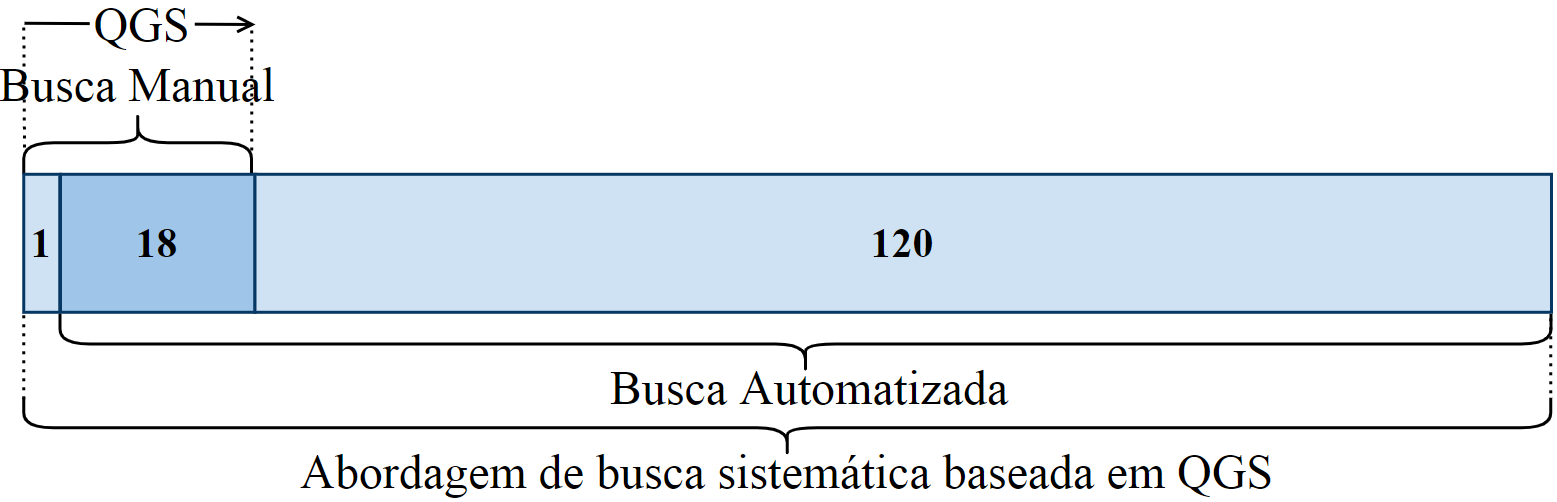
\includegraphics[width=.9\textwidth]{images/chapter2-sm-qgs-search.png}
\fautor
\end{figure}

Para extrair as informações relevantes dos estudos primários identificados, um formulário de extração de dados foi criado. A \autoref{method:table:data-extraction} representa o modelo que descreve as informações extraídas e apresenta seu relacionamento com cada QP, quando aplicável.

\sigla*{SWEBOK}{\textit{Software Engineering Body of Knowledge}}
\sigla*{ES}{Engenharia de Software}

\begin{table}[htb]
\centering
\caption{Formulário de Extração de Dados.}
\label{method:table:data-extraction}
\begin{tabular}{lll} \hline
\textbf{Item} & \textbf{Descrição} & \textbf{QP} \\ \hline
\textit{\textbf{Informações Gerais}} & & \\ \hline
ID & Identificador (prefixos \textit{INT} ou \textit{BRA}). & \\
Título & Título do estudo. & \\
Autores & Nomes dos autores. & \\
Ano & Ano de publicação do artigo. & \\
Conferência/Periódico & Nome do meio de publicação. & \\
Tipo de busca & Manual; Automatizada; Ambas. & \\
Língua & Inglês; Português. & \\
País & País da afiliação do primeiro autor. & \\ \hline
\textit{\textbf{Informações Específicas}} & & \\ \hline
Área da Eng. de Software (ES) & Área de conhecimento da ES (SWEBOK). & QP1 \\
Tipo de solução & Software; Hardware; Teórica. & QP1 \\
Estratégia empírica & Quais estratégias empíricas foram encontradas. & QP1 \\
Tópico educacional & Quais tópicos educacionais foram encontrados. & QP2 \\
Línguas de sinais & Quais línguas de sinais foram encontradas. & QP3 \\ \hline
\end{tabular}
\end{table}

\subsection{Resultados e Discussões}
\label{ms:resultados}

Portanto, o MS contou com 185 estudos primários selecionados: 46 da busca manual nacional e 139 da busca sistemática baseada em QGS. Lembrando que, as informações mais relevantes para responder cada QP foram obtidas por meio do formulário de extração de dados. Primeiramente, considerando a quantidade de publicações por ano, uma linha de tendência linear crescente foi identificada (\autoref{results:figure:publications-year}). Portanto, é estatisticamente possível que este domínio de pesquisa esteja em ascensão globalmente.


\begin{figure}[htb]
\centering 
\caption{Linha de Tendência Linear Crescente de Publicações por Ano.}
\label{results:figure:publications-year}
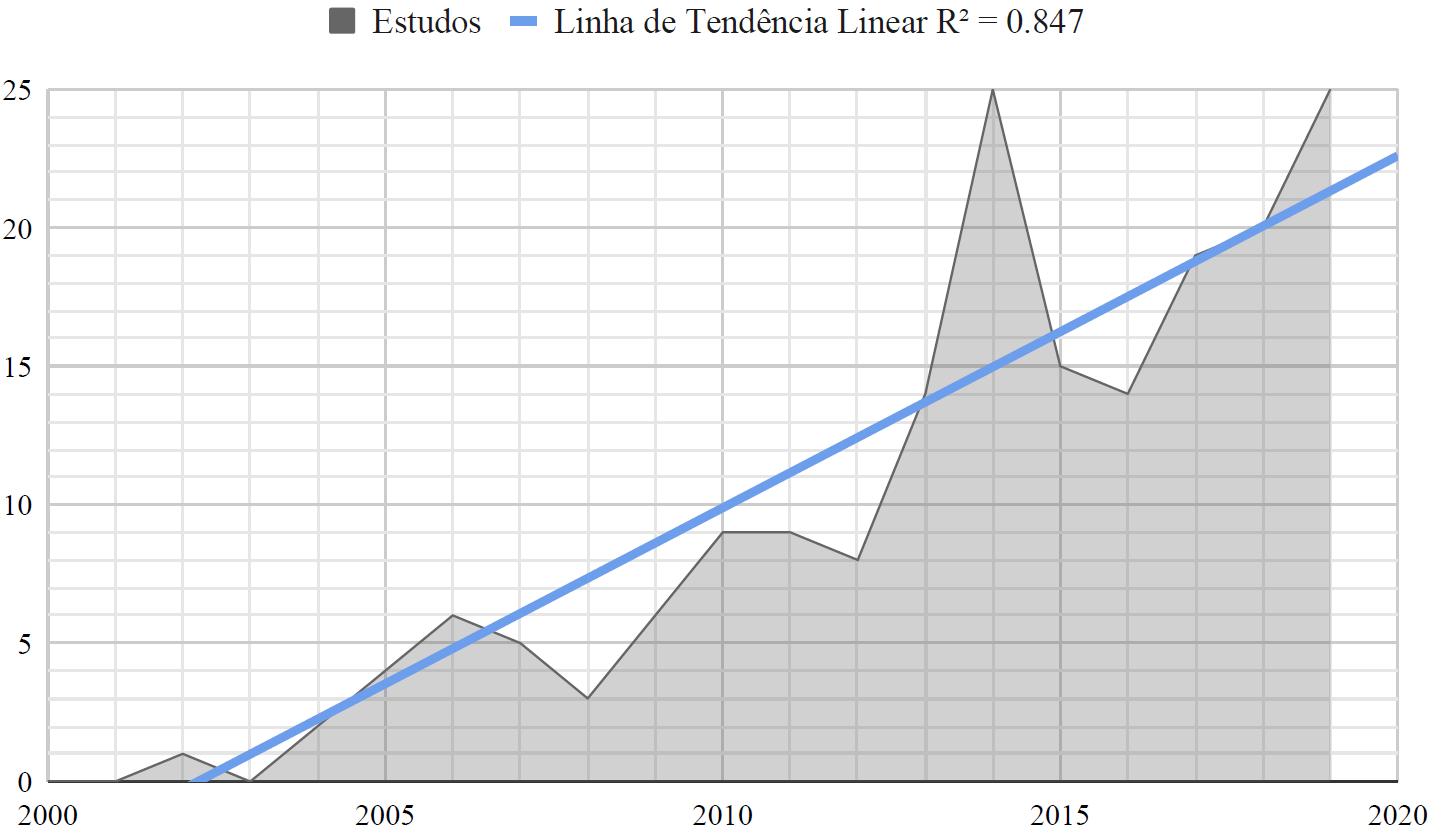
\includegraphics[width=.95\textwidth]{images/chapter2-sm-publications-timeline.png}
\fautor
\end{figure}

\simbolo{R^2}{Linha de Tendência Linear}

No que diz respeito às conferências, periódicos e fontes das publicações, esses dados também podem compor um racional interessante para futuras replicações. Sendo assim, todos os estudos primários deste MS foram ordenados pela quantidade de estudos selecionados (\autoref{results:table:publication-venues}). No contexto internacional, a presença de eventos identificados durante as buscas manuais (em \textbf{\textit{destaque}} na \autoref{results:table:publication-venues}) sugere uma execução efetiva dessa fase considerando o protocolo de busca adotado.

\begin{table}[htb]
\caption{Conferências/Periódicos mais relevantes.}
\label{results:table:publication-venues}
\centering
\begin{tabular}{lcc|lcc} \hline
\multicolumn{3}{c|}{\textbf{Internacionais (\textit{INT})}} & \multicolumn{3}{c}{\textbf{Nacionais (\textit{BRA})}} \\ \hline
\textbf{Nome} & \textbf{Fonte} & \textbf{Estudos} & \textbf{Nome} & \textbf{Fonte} & \textbf{Estudos} \\ \hline
\textit{\textbf{HCI International}} & \textit{\textbf{Springer}} & \textit{\textbf{12}} & RENOTE & CINTED & 13 \\ 
ICCHP & Springer & 8 & SBIE & CEIE & 13 \\ 
\textit{\textbf{ICALT}} & \textit{\textbf{IEEE}} & \textit{\textbf{6}} & WCBIE & CEIE & 11 \\ 
ASSETS & ACM & 6 & WIE & CEIE & 7 \\ 
\textit{\textbf{Computers \& Education}} & \textit{\textbf{Elsevier}} & \textit{\textbf{5}} & RBIE & CEIE & 2 \\ 
Procedia Computer Science & Elsevier & 5 & - & - & - \\ 
Outros & - & 97 & - & - & - \\ \hline
\multicolumn{2}{l}{\textbf{Total}} & \textbf{139} & \multicolumn{2}{l}{\textbf{Total}} & \textbf{46} \\ \hline
\end{tabular}
\end{table}

A seguir são discutidos os principais resultados deste estudo, de modo a responder cada QP definida no escopo do MS. Adicionalmente, com o objetivo de organizar os estudos primários, eles foram classificados com relação à sua origem: Internacional (\textit{INT})\footnote{Formulário de extração de dados Internacionais (INT): \url{https://bit.ly/SM-DataExtraction-INT}} ou Nacional (\textit{BRA})\footnote{Formulário de extração de dados Nacionais (BRA): \url{https://bit.ly/SM-DataExtraction-BRA}}. Com isso, os resultados podem ser analisados de forma isolada, o que facilita o planejamento e a condução de trabalhos futuros.

\subsubsection{QP1: Quais soluções tecnológicas vêm sendo propostas no processo de ensino-aprendizagem com línguas de sinais?}

As áreas presentes na \autoref{results:table:se-areas} destacam a importância intrínseca das arquiteturas de software na construção de TAs para línguas de sinais. Embora haja uma concentração significativa nas etapas de ``Construção'' e ``Projeto'', poucas soluções se mostraram realmente replicáveis ou adaptáveis a diferentes contextos educacionais, principalmente pela falta de detalhes técnicos.

\begin{table}[htb]
\caption{QP1: Áreas da ES no SWEBOK \cite{Bourque2014}.}
\label{results:table:se-areas}
\centering
\begin{tabular}{lcc|cc} \hline
 & \multicolumn{2}{c|}{\textit{\textbf{INT}}} & \multicolumn{2}{c}{\textit{\textbf{BRA}}} \\ \cline{2-5} 
\textbf{Área da ES} & \textbf{Estudos} & \textbf{\%} & \textbf{Estudos} & \textbf{\%} \\ \hline
Construção de Software & 65 & 47\% & 23 & 50\% \\
Projeto de Software & 47 & 34\% & 5 & 11\% \\
Fundamentos da Engenharia & 24 & 17\% & 9 & 19\% \\
Qualidade de Software & 3 & 2\% & 9 & 19\% \\ \hline
\textbf{Total} & \textbf{139} & \textbf{100\%} & \textbf{46} & \textbf{100\%} \\ \hline
\end{tabular}
\end{table}

Tecnicamente, a grande maioria das soluções é baseada em plataformas Web, Mobile ou Desktop, evidenciando uma preocupação genuína em criar TAs para diferentes plataformas de ensino-aprendizagem. No entanto, poucos estudos foram estruturados de forma a facilitar o seu reuso e extensibilidade. Além disso, menos da metade dos estudos apresentou avaliações empíricas formais, como \textit{Surveys}, Experimentos e Estudos de Caso, indicando uma falta de rigor científico em parte das pesquisas \cite{Pressman2016, Sommerville2015}.

Em contrapartida, avatares de línguas de sinais baseados em texto, como o \textit{Hand Talk}\footnote{Mais informações em \url{https://handtalk.me}} e o \textit{VLibras}\footnote{Mais informações em \url{https://gov.br/governodigital/pt-br/vlibras}}, destacam-se ao transformar texto em língua de sinais, evidenciando o potencial de TAs bem arquitetadas para potencializar a acessibilidade de conteúdos em diversos contextos educacionais. Portanto, a discussão sobre Arquiteturas de Software na \autoref{section:foundation:arch} será fundamental para compreender como essas soluções podem ser aprimoradas para desenvolver TAs verdadeiramente escaláveis.

\subsubsection{QP2: Quais tópicos educacionais são abordados?}

A \autoref{results:table:educational-topics} apresenta uma ampla diversidade de tópicos educacionais tendo em vista os OAs analisados, evidenciando o uso de TAs para línguas de sinais em diversos contextos. O que representa um esforço consciente em abordar diferentes temas no processo de ensino-aprendizagem, promovendo uma acessibilidade digital mais ampla e personalizada. 

\begin{table}[htb]
\caption{QP2: Tópicos Educacionais.}
\label{results:table:educational-topics}
\centering
\begin{tabular}{lcc|cc} \hline
 & \multicolumn{2}{c|}{\textit{\textbf{INT}}} & \multicolumn{2}{c}{\textit{\textbf{BRA}}} \\ \cline{2-5} 
\textbf{Tópico Educacional} & \textbf{Estudos} & \textbf{\%} & \textbf{Estudos} & \textbf{\%} \\ \hline
Línguas de Sinais & 59 & 42,5\% & 19 & 41,3\% \\
Geral & 48 & 34,5\% & 10 & 21,7\% \\
Língua de Sinais Escrita & 10 & 7,2\% & 3 & 6,5\% \\
Matemática & 7 & 5,0\% & - & - \\
Alfabeto & 6 & 4,3\% & 1 & 2,2\% \\
Ciência da Computação & 4 & 2,9\% & 4 & 8,7\% \\
Língua Falada do País & 2 & 1,4\% & 9 & 19,6\% \\
Outros & 3 & 2,2\% & - & - \\ \hline
\textbf{Total} & \textbf{139} & \textbf{100\%} & \textbf{46} & \textbf{100\%} \\ \hline
\end{tabular}
\end{table}

Com uma vasta gama de OAs inclusivos e adaptáveis, os educadores podem proporcionar experiências de aprendizado mais imersivas e eficazes, garantindo oportunidades igualitárias de desenvolvimento para todos os alunos, independentemente de suas habilidades ou desafios individuais. Tais resultados estabelecem a base para uma discussão mais aprofundada sobre OAs na \autoref{section:foundation:lo}, onde exploraremos como esses recursos podem ser projetados para atender demandas educacionais diversas.

\subsubsection{QP3: Quais línguas de sinais são abordadas?}

\sigla*{IAGen}{Inteligências Artificiais Generativas}

As línguas de sinais mais comuns, destacadas na \autoref{results:table:sign-languages}, juntamente com o crescente interesse em ASR multilíngue, abrem caminho para avanços significativos na acessibilidade. A capacidade das IAs Generativas (IAGen) de transcrever e traduzir fala em texto em múltiplas línguas viabiliza a integração de avatares de línguas de sinais baseados em texto, resultando em OAs mais inclusivos e versáteis.

\begin{table}[htb]
\caption{QP3: Línguas de Sinais.}
\label{results:table:sign-languages}
\centering
\begin{tabular}{lcc|cc} \hline
 & \multicolumn{2}{c|}{\textit{\textbf{INT}}} & \multicolumn{2}{c}{\textit{\textbf{BRA}}} \\ \cline{2-5} 
\textbf{Língua de Sinais} & \textbf{Estudos} & \textbf{\%} & \textbf{Estudo} & \textbf{\%} \\ \hline
ASL & 21 & 15.11\% & - & - \\
Libras & 16 & 11.51\% & 44 & 95.65\% \\
Geral & 15 & 10.79\% & - & - \\
SignWriting & 10 & 7.19\% & 2 & 4.35\% \\
ArSL & 10 & 7.19\% & - & - \\
PSL & 6 & 4.32\% & - & - \\
BSL & 6 & 4.32\% & - & - \\
MySL & 6 & 4.32\% & - & - \\
ISL & 5 & 3.60\% & - & - \\
Outras & 44 & 31.65\% & - & - \\ \hline
\textbf{Total} & \textbf{139} & \textbf{100\%} & \textbf{46} & \textbf{100\%} \\ \hline
\end{tabular}
\end{table}

Nesse cenário, línguas de sinais como a \textit{American Sign Language} (ASL) e a Libras, além de sistemas de escrita como o \textit{SignWriting}, podem se beneficiar dessas tecnologias, ampliando o acesso a conteúdos educacionais antes restritos aos formatos de áudio e vídeo. Esses resultados ressaltam a importância do ASR, que será aprofundado na \autoref{section:foundation:asr}.

A análise dos resultados obtidos pelas QP fornece um panorama do uso das TICs no ensino e aprendizado com línguas de sinais, revelando tanto lacunas quanto oportunidades para avanços significativos na criação de TAs ainda mais robustas. Essas descobertas abrem caminho para uma exploração detalhada de temas cruciais, como Arquiteturas de Software (\autoref{section:foundation:arch}), OAs (\autoref{section:foundation:lo}) e ASR (\autoref{section:foundation:asr}). Cada seção subsequente destaca como suas temáticas podem ajudar a superar os desafios identificados e a capitalizar nas oportunidades emergentes, contribuindo para um processo de ensino-aprendizagem mais inclusivo e acessível.

\section{Arquiteturas de Software: Bases Sólidas para Tecnologias Assistivas}
\label{section:foundation:arch}

Uma das principais lacunas identificadas no MS foi a carência de padrões e boas práticas que permitam o reuso e a adaptação das soluções no ensino e aprendizagem com línguas de sinais. Muitos dos estudos primários apresentaram contribuições técnicas relevantes, mas não detalharam as arquiteturas de software utilizadas, dificultando a evolução e derivação dessas soluções para outros contextos e domínios de aplicação. Por isso, discutiremos como as arquiteturas podem contribuir para o desenvolvimento de TAs replicáveis, flexíveis e independentes de tecnologia, seguindo alguns princípios e diretrizes da ES.

Nesse sentido, uma arquitetura de software pode ser definida como o conjunto de estruturas necessárias para o entendimento de um sistema, compreendendo desde seus componentes de software e hardware até suas relações/propriedades internas e externas \cite{Bass2021}. Essa definição enfatiza que a arquitetura não se limita apenas a decisões iniciais, mas inclui todas as decisões que moldam a estrutura do projeto e suas interações. A arquitetura é fundamental para a criação de sistemas complexos e facilita a análise de requisitos não funcionais, como desempenho, segurança e escalabilidade \cite{Pressman2016, Sommerville2015}.

Diferentemente de outras definições focadas em decisões antecipadas, a arquitetura, conforme \citeonline{Bass2021}, é sobre estruturas que permitem o raciocínio e a análise do sistema. Essa perspectiva permite uma compreensão mais ampla e flexível da arquitetura, considerando suas múltiplas dimensões e aspectos envolvidos no desenvolvimento e manutenção do software.

\subsection{Estruturas e Visões Arquiteturais}

Resumidamente, a arquitetura pode ser vista como um conjunto de estruturas que proporcionam diferentes perspectivas sobre o sistema, cada uma com seu foco específico, o qual pode ser necessário em diferentes fases do ciclo de vida do software. Formalmente, \citeonline{Bass2021} identificam três tipos principais de estruturas arquiteturais, que formam as principais visões neste contexto:

\begin{itemize}

    \item \textbf{Estruturas de Componentes e Conectores (C\&C)}: Estas estruturas focam nas interações em tempo de execução entre os componentes que realizam as funções do sistema. Componentes, que podem ser serviços, clientes, servidores ou filtros, são as unidades principais de computação. Os conectores, por sua vez, são os veículos de comunicação entre esses componentes, facilitando a troca de dados e a sincronização de processos. As estruturas C\&C são cruciais para entender o comportamento em tempo de execução, incluindo a interação entre componentes, a replicação de partes do sistema e a paralelização de tarefas \cite{Bass2021};
    
    \item \textbf{Estruturas de Módulos}: Estas estruturas particionam o sistema em unidades de implementação, conhecidas como módulos, que são responsáveis por funções específicas e são a base para a organização do trabalho de desenvolvimento. Módulos podem representar classes, pacotes ou divisões de funcionalidade, cada um com um papel definido no sistema. As relações entre os módulos, como uso, generalização e composição, ajudam a entender a estrutura estática do sistema e a gerenciar sua evolução e manutenção \cite{Bass2021};
    
    \item \textbf{Estruturas de Alocação}: Estas estruturas estabelecem a correspondência entre as estruturas de software e os componentes não software do sistema, como ambientes de desenvolvimento e execução. Elas respondem a questões críticas sobre onde cada elemento de software será executado, como os elementos estão armazenados e como são atribuídos às equipes de desenvolvimento. As estruturas de alocação são essenciais para a compreensão da distribuição do software e para a gestão de recursos durante todo o ciclo de vida do sistema \cite{Bass2021}.
    
\end{itemize}

Essas estruturas arquiteturais são análogas às diferentes especialidades médicas que focam em partes específicas do corpo humano, como ilustra a \autoref{chapter2:figure:physiological-structures}. Essa analogia facilita a compreensão de como diferentes visões se complementam para fornecer uma compreensão abrangente do sistema como um todo \cite{Bass2021}.

\begin{figure}[htb]
\centering
\caption{Fisiologia Humana: Análoga às Estruturas e Visões Arquiteturais}
\label{chapter2:figure:physiological-structures}
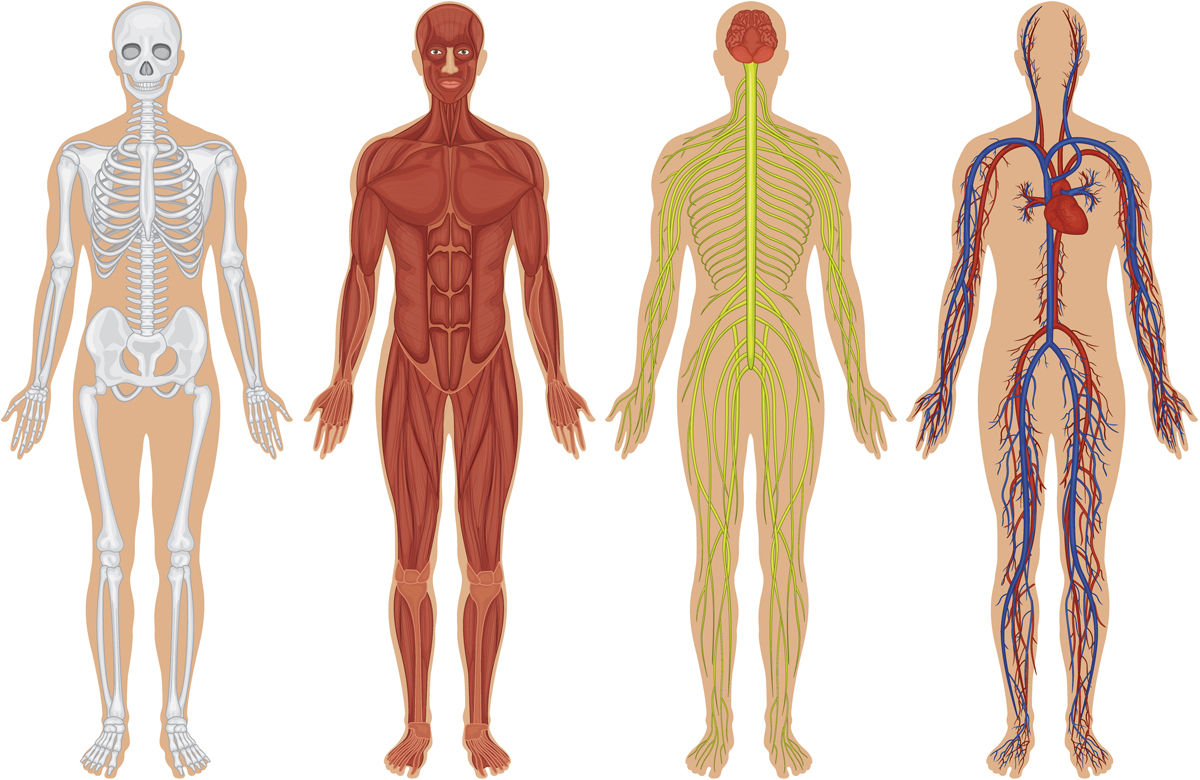
\includegraphics[width=0.60\textwidth]{images/chapter2-arch-physiological-structures.jpeg}
\end{figure}

Essas três categorias de estruturas facilitam a criação de representações visuais que auxiliam na compreensão da arquitetura de software em diferentes etapas do desenvolvimento. A arquitetura \textit{Speech2Learning}, por exemplo, adota essas estruturas para garantir clareza arquitetural desde sua concepção até a avaliação em seus estudos de caso (detalhes nos Capítulos \ref{chapter3} e \ref{chapter4}). Essa abordagem sistematiza e torna mais eficiente a implementação de TAs.

\subsection{O que Torna uma Arquitetura ``Boa''?}

Na prática, a arquitetura de software é uma abstração que destaca detalhes relevantes para a compreensão e análise do sistema, omitindo informações desnecessárias para o raciocínio sobre ele. A abstração é crucial para gerir a complexidade, permitindo que arquitetos e desenvolvedores se concentrem em aspectos essenciais sem se preocuparem com detalhes de implementação. A arquitetura trata dos elementos públicos do sistema, ou seja, aqueles que interagem entre si através de interfaces, enquanto os detalhes privados de implementação não são considerados \cite{Bass2021}.

Padrões arquiteturais são composições de elementos arquiteturais que foram documentadas e disseminadas devido à sua eficácia em resolver problemas recorrentes em diferentes domínios. Esses padrões fornecem abordagens comprovadas para o design de sistemas e são fundamentais para alcançar os atributos de qualidade desejados, como modularidade e facilidade de manutenção \cite{Bass2021}. Por exemplo, o padrão de arquitetura em camadas é amplamente utilizado para sistemas que necessitam de alta modularidade, enquanto o padrão de microsserviços é ideal para sistemas que requerem escalabilidade e resiliência \cite{Pressman2016, Sommerville2015}.

Entretanto, não existe uma arquitetura intrinsecamente ``boa'' ou ``ruim''; a adequação de uma arquitetura depende de como ela atende aos requisitos específicos do sistema. Uma arquitetura projetada para um sistema de comércio eletrônico pode não ser adequada para um sistema de controle de voo, por exemplo. A avaliação da arquitetura em relação a objetivos específicos é crucial para garantir que ela atenda às necessidades do sistema \cite{Pressman2016, Sommerville2015}.

Para orientar o desenvolvimento de uma boa arquitetura de software, \citeonline{Bass2021} propõem algumas boas práticas, categorizadas em recomendações de processo e estruturais. Primeiramente, as \textbf{recomendações de processo} focam na maneira como a arquitetura deve ser desenvolvida e gerenciada ao longo do ciclo de vida do sistema, garantindo que a integridade conceitual e a qualidade sejam mantidas de forma contínua:

\begin{enumerate}
    \item \textbf{Desenvolvimento por lideranças técnicas}: É fundamental que a arquitetura seja concebida por um arquiteto ou uma pequena equipe de arquitetos com um líder técnico identificado, garantindo a integridade conceitual e a consistência técnica. Esse princípio também se aplica a projetos ágeis e de código aberto, evitando designs impraticáveis e desconectados da realidade do desenvolvimento.
    
    \item \textbf{Foco nos requisitos de qualidade}: A arquitetura deve se basear continuamente em uma lista priorizada de requisitos de qualidade bem definidos. Esses requisitos informam as decisões de \textit{trade-offs} que sempre ocorrem, sendo mais relevantes do que a funcionalidade em si.
    
    \item \textbf{Documentação por meio de visões arquiteturais}: A arquitetura deve ser documentada através de visões que representem uma ou mais estruturas arquiteturais. Essas visões devem abordar as preocupações dos \textit{stakeholders} mais importantes e apoiar o cronograma do projeto, fornecendo uma documentação que pode ser inicialmente minimalista, mas detalhada posteriormente.
    
    \item \textbf{Avaliação contínua dos atributos de qualidade}: A arquitetura deve ser avaliada quanto à sua capacidade de fornecer os principais atributos de qualidade do sistema. Isso deve ocorrer no início do ciclo de vida, proporcionando os maiores benefícios, e ser repetido conforme necessário para garantir que alterações na arquitetura ou no ambiente não tornem o design obsoleto.
    
    \item \textbf{Implementação incremental e adaptativa}: A arquitetura deve permitir a implementação incremental, evitando a integração total de uma só vez, o que raramente funciona. Isso pode ser alcançado através da criação de um sistema esquelético, no qual os caminhos de comunicação são exercidos inicialmente com funcionalidade mínima, permitindo o crescimento incremental do sistema e a refatoração conforme necessário.
\end{enumerate}

Por sua vez, as \textbf{recomendações estruturais} dizem respeito à organização interna da arquitetura, enfatizando a importância da modularidade, da separação de responsabilidades e da flexibilidade na integração dos componentes, visando a criação de um sistema robusto e facilmente evolutivo:

\begin{enumerate}
    \item \textbf{Modularização e separação de preocupações}: A arquitetura deve apresentar módulos bem definidos, cujas responsabilidades funcionais são atribuídas com base nos princípios de ocultação de informações e separação de preocupações. Esses módulos devem encapsular aspectos passíveis de mudança, isolando o software dos efeitos dessas mudanças.
    
    \item \textbf{Uso de padrões arquiteturais bem estabelecidos}: A arquitetura deve alcançar atributos de qualidade usando padrões arquiteturais e táticas bem estabelecidos e específicos para cada atributo. Isso proporciona uma base sólida para o design, garantindo que os requisitos de qualidade sejam atendidos de maneira eficaz.
    
    \item \textbf{Flexibilidade em relação a versões de produtos}: A arquitetura nunca deve depender de uma versão específica de um produto comercial ou ferramenta. Se isso for inevitável, deve ser estruturada de forma que a mudança para uma versão diferente seja simples e barata.
    
    \item \textbf{Separação entre componentes produtores e consumidores de dados}: Os módulos que produzem dados devem ser separados dos módulos que consomem esses dados. Isso aumenta a manutenibilidade, permitindo que mudanças sejam confinadas ao lado da produção ou do consumo de dados, facilitando atualizações incrementais.
    
    \item \textbf{Flexibilidade na correspondência entre módulos e componentes}: Não se deve esperar uma correspondência um-para-um entre módulos e componentes. Em sistemas com concorrência, por exemplo, múltiplas instâncias de um componente podem ser executadas em paralelo, cada uma construída a partir do mesmo módulo.
    
    \item \textbf{Alocação flexível de processos}: Projete cada processo para ser executado em qualquer processador, permitindo fácil realocação, inclusive durante a execução. Isso é essencial em ambientes de virtualização e nuvem, onde os recursos computacionais podem variar.
    
    \item \textbf{Consistência e simplicidade nos padrões de interação}: A arquitetura deve conter um pequeno número de padrões simples de interação entre componentes. O sistema deve realizar as mesmas funções da mesma maneira em todas as partes, o que facilita a compreensão, reduz o tempo de desenvolvimento, além de aumentar confiabilidade e manutenibilidade.
    
    \item \textbf{Gestão eficaz de áreas de contenção de recursos}: A arquitetura deve conter um conjunto específico e pequeno de áreas de contenção de recursos, cuja resolução deve ser claramente especificada e mantida. Por exemplo, se a utilização da rede é uma preocupação, o arquiteto deve produzir diretrizes para cada equipe de desenvolvimento que resultem em níveis aceitáveis de tráfego de rede.
\end{enumerate}

Em suma, uma arquitetura de software bem projetada não só atende aos requisitos funcionais imediatos, mas também oferece uma base sólida que permite a evolução e adaptação contínua do sistema, especialmente em áreas críticas como a educação inclusiva. A flexibilidade da arquitetura é essencial para suportar a evolução contínua das TICs e a adaptação às necessidades dos aprendizes, garantindo que as soluções sejam sustentáveis e capazes de atender às necessidades dos alunos a longo prazo.

Nesse contexto, a arquitetura \textit{Speech2Learning} surge como uma proposta para impulsionar a construção de TAs. Projetada para integrar soluções de ASR, ela visa facilitar a criação de OAs mais acessíveis a uma ampla gama de aprendizes \cite{FalvoJr2023_HICSS}. Nos próximos capítulos, exploraremos em detalhes os conceitos de OAs e ASR, aprofundando nosso entendimento sobre como essas tecnologias se entrelaçam e formam a base da \textit{Speech2Learning}.

\section{Objetos de Aprendizagem: Diversidade em Conteúdos Educacionais}
\label{section:foundation:lo}

A diversidade em conteúdos educacionais é uma necessidade cada vez mais reconhecida, como evidenciado em nosso MS. Sendo assim, os OAs emergem como uma solução promissora para atender a essa demanda, permitindo a criação de recursos personalizados e adaptáveis a diferentes contextos e públicos. No âmbito da arquitetura \textit{Speech2Learning}, os OAs desempenham um papel fundamental no acesso a materiais didáticos audíveis, enriquecidos pela tecnologia de ASR para maior acessibilidade \cite{FalvoJr2023_HICSS}.

Os OAs abrangem um amplo espectro de recursos digitais projetados para enriquecer o processo de ensino-aprendizagem. Eles vão além da mera entrega de conteúdo, proporcionando uma experiência mais rica e interativa \cite{Wiley2000}. A importância da multimídia no aprendizado é destacada por \citeonline{Mayer2021}, que argumenta que a combinação eficaz de texto, áudio, vídeo e elementos interativos pode potencializar a retenção e aplicação do conhecimento.

\sigla*{IEEE}{\textit{Institute of Electrical and Electronics Engineers}}

O \citeonline{LOM2000} define os OAs como entidades, digitais ou não-digitais, que podem ser usadas, reutilizadas ou referenciadas durante o ensino com suporte tecnológico. Essa definição abrange uma vasta gama de recursos, incluindo conteúdos multimídia, software instrucional, eventos educacionais, entre outros. \citeonline{Wiley2000} simplifica essa concepção ao descrever os OAs como recursos digitais que podem ser reutilizados para facilitar a aprendizagem, destacando a adaptabilidade e a reusabilidade como características centrais dos OAs.

A essência dos OAs reside na criação de pequenos módulos instrucionais reutilizáveis, combináveis de diferentes maneiras para atender às necessidades específicas de aprendizagem. Essa abordagem permite que educadores personalizem o ensino, adaptando materiais didáticos às suas metas pedagógicas individuais. O resultado é um processo de ensino-aprendizagem mais dinâmico, onde diferentes recursos se conectam para formar um todo coeso (\autoref{chapter2:figure:lo-mindmap}).

\begin{figure}[htb]
\centering
\caption{Mapa Conceitual Sobre Objetos de Aprendizagem}
\label{chapter2:figure:lo-mindmap}
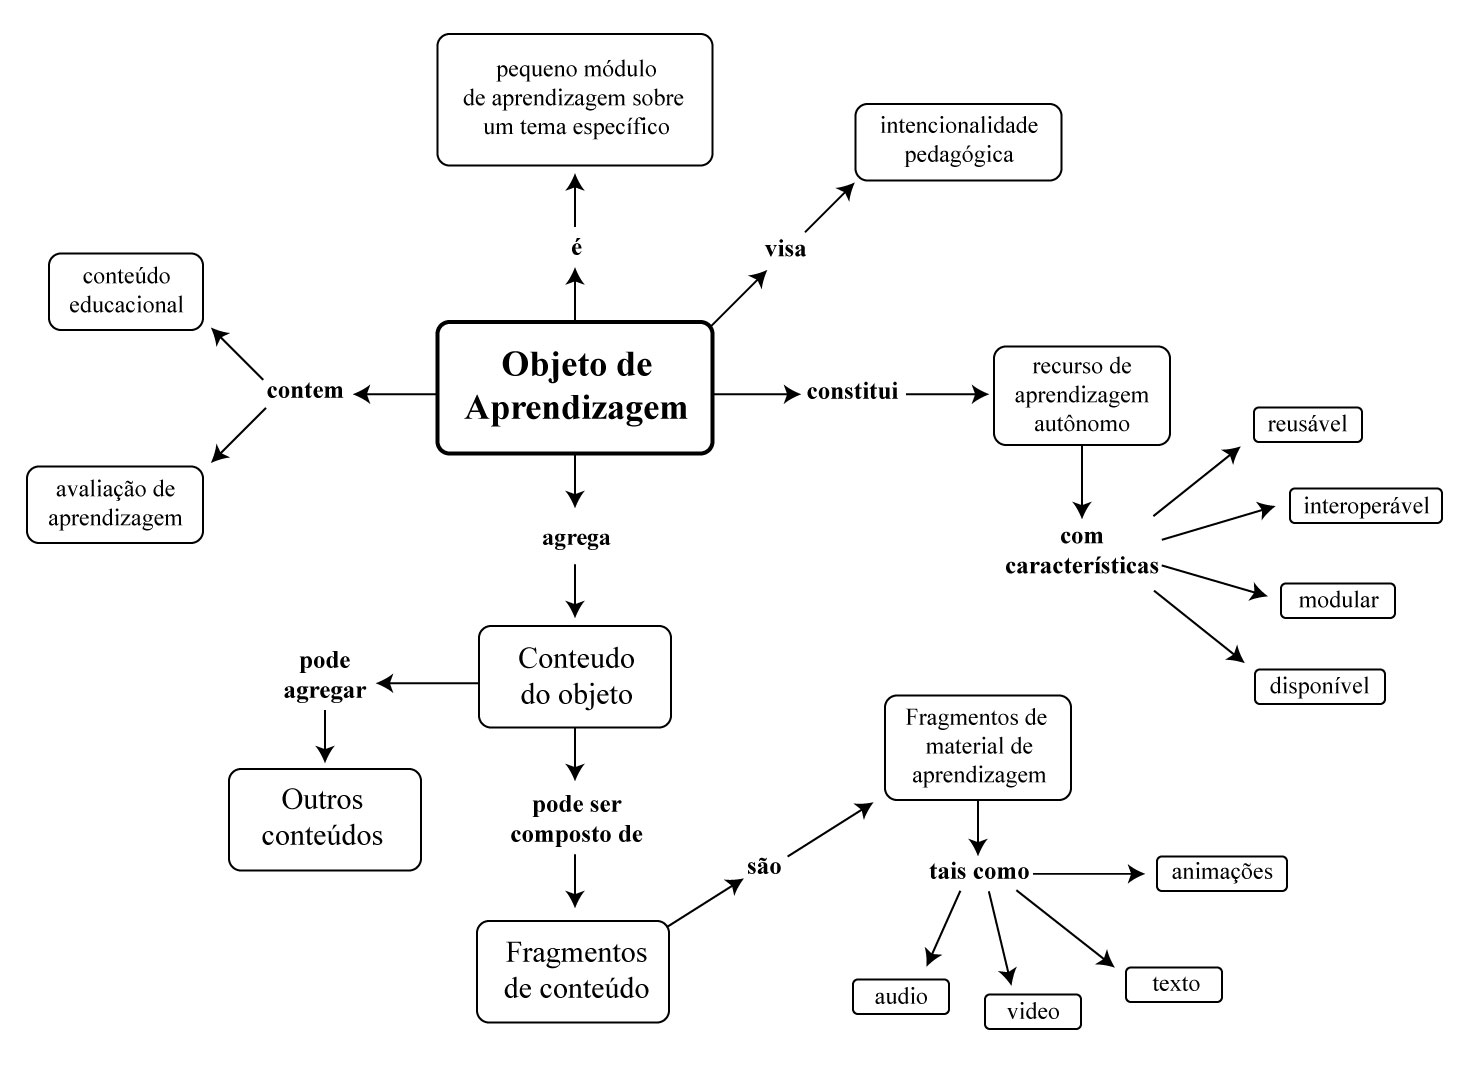
\includegraphics[width=0.88\textwidth]{images/chapter2-lo-mindmap.jpg}
\fadaptada{Tarouco2021}
\end{figure}

\subsection{Estratégias de Identificação e Utilização de OAs}

O uso e reuso de OAs envolve várias estratégias que facilitam sua adaptação a diferentes contextos educacionais. Conforme discutido por \citeonline{Tarouco2021}, os OAs podem variar em tamanho, escopo e nível de granularidade, afetando diretamente sua reusabilidade (\autoref{chapter2:figure:lo-granularity}). Objetos com granularidade fina, como imagens ou pequenos vídeos, são mais fáceis de reutilizar devido à sua simplicidade e especificidade. Em contraste, OAs de granularidade grande, como cursos, oferecem uma experiência educacional mais completa e integrada, mas são mais difíceis de adaptar a novos contextos de ensino-aprendizagem.

\begin{figure}[htb]
\centering
\caption{Granularidade de Objetos de Aprendizagem}
\label{chapter2:figure:lo-granularity}
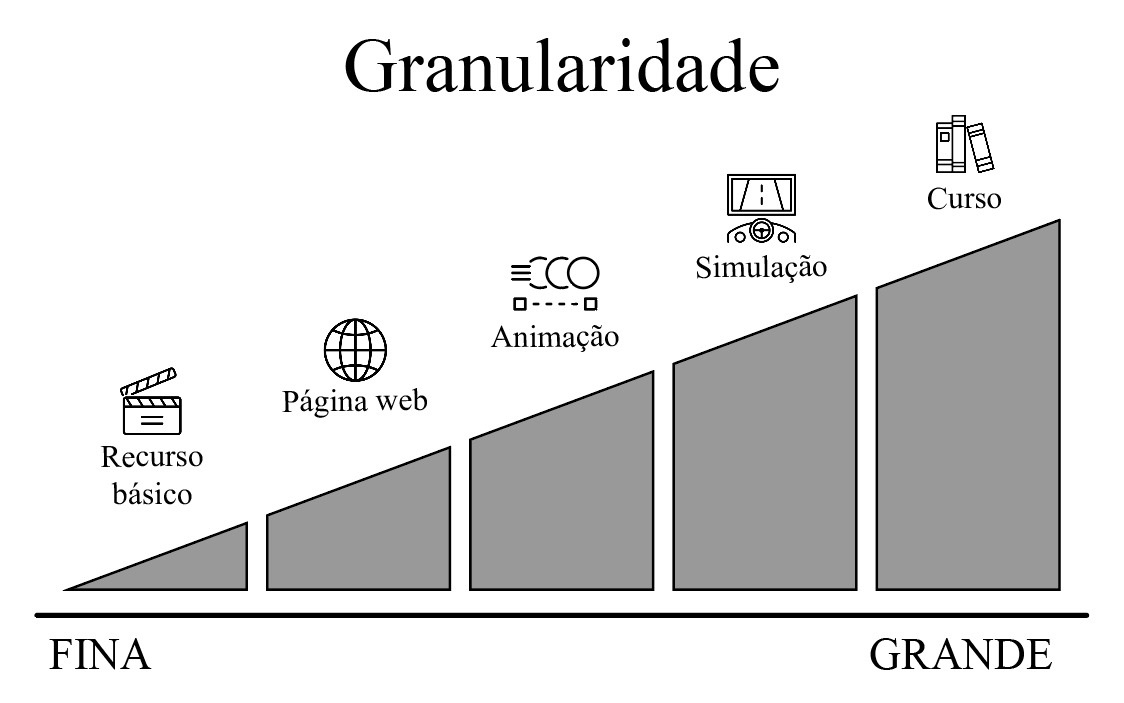
\includegraphics[width=0.7\textwidth]{images/chapter2-lo-granularity.jpeg}
\fadaptada{Tarouco2021}
\end{figure}

A granularidade dos OAs está intimamente ligada à intencionalidade pedagógica, definida pela finalidade educacional para a qual o objeto foi criado. De acordo com \citeonline{Bloom1984}, a eficácia de um OA depende da clareza de seus objetivos pedagógicos e da adequação às necessidades dos estudantes. Dessa forma, a escolha de OAs deve considerar tanto a granularidade quanto a intencionalidade pedagógica para garantir uma aprendizagem eficaz e significativa.

Nesse sentido, a adoção de padrões de metadados é essencial para a organização, indexação e reutilização de OAs. \citeonline{Santana2023} destacam a importância desses padrões e sua aplicabilidade no contexto da ES experimental, cujo compartilhamento de OAs é vital para replicações e pesquisas futuras. A \autoref{chapter2:table:lo-metadata} apresenta uma comparação entre vários padrões de metadados, destacando suas características principais:

\begin{itemize}
    \item \textit{Dublin Core}\footnote{Mais informações em \url{https://dublincore.org}}: Um padrão internacional que fornece um conjunto simples e padronizado de termos para descrever recursos. O Dublin Core é conhecido por sua simplicidade e extensibilidade, permitindo sua aplicação em diversos contextos, desde bibliotecas digitais até sistemas de informação corporativos.
    \item \sigla{SCORM}{\textit{Sharable Content Object Reference Model}}\footnote{Mais informações em \url{https://adlnet.gov/scorm}}: Um conjunto de padrões e especificações para e-learning que define a comunicação entre o conteúdo de aprendizado online e os sistemas de gerenciamento de aprendizado (LMS). Desenvolvido pela Advanced Distributed Learning (ADL), o SCORM facilita a interoperabilidade e a reutilização de conteúdos educacionais em diferentes plataformas de aprendizado.
    \item \textit{Motion Imagery Standard Board} (MISB)\footnote{Mais informações em \url{https://nsgreg.nga.mil/misb.jsp}}: Padrão desenvolvido para a gestão e utilização de imagens em movimento, particularmente em contextos que exigem alta precisão e interoperabilidade, como vigilância e análise de vídeo. O MISB, parte da \textit{National Geospatial-Intelligence Agency} (NGA), assegura que os dados de vídeo sejam consistentes e compatíveis em diferentes sistemas.
    \item \sigla{LOM}{\textit{Learning Object Metadata}}\footnote{Mais informações em \url{https://ieeexplore.ieee.org/document/9262118}}: Um padrão para a descrição de metadados de OAs, abrangendo aspectos como a finalidade educacional, estrutura, nível de agregação e condições de uso. Publicado pelo IEEE, o LOM é amplamente utilizado para descrever e categorizar recursos educacionais digitais, facilitando sua descoberta e reutilização.
    \item \sigla{RDF}{\textit{Resource Description Framework}}\footnote{Mais informações em \url{https://w3.org/rdf}}: Uma especificação da W3C que fornece uma base para a descrição de recursos da web. O RDF é utilizado para modelagem de informações, permitindo a interoperabilidade entre diferentes sistemas de informação e facilitando a integração de dados de diversas fontes.
\end{itemize}

\begin{table}[htb]
\caption{Comparação Entre os Padrões de Metadados} 
\label{chapter2:table:lo-metadata}
\begin{tabular}{|P{3.5cm}|P{3cm}|P{3cm}|P{3cm}|}\hline
\textbf{Padrão de Metadados} & \textbf{Documentação Completa} & \textbf{Processamento Automatizado} & \textbf{Flexibilidade para ES} \\ \hline
Dublin Core & X & X & X \\  \hline
SCORM & X & X & X \\ \hline
MISB & X & X & \\ \hline
LOM & X & X & X \\ \hline
RDF & X & X & X \\ \hline
\end{tabular}
\fadaptada{Santana2023}
\end{table}

Segundo \citeonline{Santana2023}, o Dublin Core se destaca por sua simplicidade, documentação abrangente e capacidade de processamento automatizado, permitindo sua aplicação em diferentes linhas de pesquisa na área da ES. No entanto, no contexto deste trabalho, qualquer padrão de metadados pode ser adequado, visto que o papel de uma arquitetura de software não é o de definir ``detalhes de implementação''. 

Por outro lado, o LOM merece destaque pelo seu foco intrínseco em aspectos educacionais, demonstrando uma sinergia natural com o conceito de OAs. Além disso, com exceção do MISB, todos os padrões são tão robustos quanto o Dublin Core, considerando os critérios de comparação da \autoref{chapter2:table:lo-metadata}.

Ao conhecer os conceitos de granularidade e padrões de metadados, fica mais simples entendermos como os OAs podem ser encontrados. Nesse sentido, os Repositórios de Objetos de Aprendizagem (ROAs) são plataformas que armazenam e disponibilizam OAs para educadores, estudantes e desenvolvedores. Eles desempenham um papel crucial na disseminação de recursos educacionais e na promoção do uso e reuso de OAs. No Brasil, de acordo com \citeonline{Tarouco2021}, alguns dos principais ROAs incluem: \textit{Portal do Professor}\footnote{Mais informações em \url{http://portaldoprofessor.mec.gov.br}}, \textit{Domínio Público}\footnote{Mais informações em \url{http://www.dominiopublico.gov.br}} e \textit{eduCAPES} \footnote{Mais informações em \url{https://educapes.capes.gov.br}}.

A utilização de padrões de metadados, como o LOM, nesses repositórios facilita a indexação e a busca eficiente de OAs, permitindo que educadores encontrem rapidamente os recursos que atendam às suas necessidades pedagógicas. A combinação de granularidade adequada e metadados padronizados assegura que os OAs possam ser reutilizados em diversos contextos educacionais, maximizando seu impacto e alcance.

%Um exemplo prático da adaptabilidade dos OAs é a inclusão de transcrições em materiais audíveis, como videoaulas. Essa prática não apenas flexibiliza o acesso à informação para todos os alunos, mas também destaca a capacidade dos OAs de se adaptarem às necessidades de uma gama diversificada de aprendizes, promovendo uma educação mais inclusiva. O potencial de adaptação dos OAs reforça a importância das TICs, como o ASR, na ampliação da acessibilidade e personalização dos conteúdos educacionais, conforme identificado no MS como um \textit{insight} relevante para a concepção da arquitetura \textit{Speech2Learning} \cite{FalvoJr2023_HICSS}.

A granularidade, os padrões de metadados e os repositórios de OAs convergem para apoiar a intencionalidade pedagógica. A intencionalidade pedagógica, por sua vez, refere-se à finalidade educacional para a qual os OAs são criados e utilizados. De acordo com \citeonline{Bloom1984}, a eficácia de um OA depende da clareza de seus objetivos pedagógicos e da adequação às necessidades dos estudantes.

A próxima seção discorrerá sobre a intencionalidade pedagógica, exemplificando como a Taxonomia de Bloom e sua revisão podem ser aplicadas na seleção e utilização de OAs para maximizar o processo de ensino-aprendizagem.

\subsection{Intencionalidade Pedagógica}

A intencionalidade pedagógica dos OAs pode ser exemplificada pela Taxonomia de Bloom, que categoriza objetivos educacionais em uma hierarquia de complexidade cognitiva \cite{Bloom1984}. Em um trabalho mais recente, \citeonline{Krathwohl2002} propôs uma revisão da taxonomia original, estruturando-a em uma perspectiva bi-dimensional. A primeira dimensão é a do conhecimento, que se desdobra em quatro tipos:

\begin{itemize}
    \item \textbf{Factual}: conhecimento básico de terminologias e detalhes específicos;
    \item \textbf{Conceitual}: inter-relações entre os elementos básicos em uma estrutura maior;
    \item \textbf{Procedimental}: métodos e critérios para realizar tarefas e resolver problemas;
    \item \textbf{Metaconhecimento}: conhecimento sobre o próprio conhecimento e sua regulação.
\end{itemize}

A segunda dimensão trata dos processos cognitivos, referida como Taxonomia de Bloom Revisada, que propõem seis categorias adaptadas da taxonomia original de \citeonline{Bloom1984}. \citeonline{Krathwohl2002} introduziu mudanças significativas, com destaque para o uso de verbos ativos em vez de substantivos e a reestruturação de alguns dos níveis. Como resultado, a nova versão organiza os OAs nas seguintes categorias:

\begin{itemize}
    \item \textbf{Recordar}: Capacidade de reter conhecimento na memória de longo prazo;
    \item \textbf{Entender}: Capacidade de construir significado a partir do material instrucional;
    \item \textbf{Aplicar}: Capacidade de utilizar o(s) procedimento(s) adequado(s) à situação vivenciada;
    \item \textbf{Analisar}: Capacidade de identificar diferentes partes constituintes de um material compreendendo suas inter-relações;
    \item \textbf{Avaliar}: Capacidade de estabelecer julgamentos a partir de critérios e padrões;
    \item \textbf{Criar}: Capacidade de transpor o conhecimento construído para novas situações a partir de produtos originais de autoria do próprio estudante.
\end{itemize}

Em virtude da representação bidimensional dos OAs propostos pela Taxonomia de Bloom Revisada, optou-se por adotar o uso de uma tabela de duas dimensões (\autoref{chapter2:lo:los-categories}) para a classificação destes objetivos. Na tabela proposta, a dimensão do conhecimento é representada pelo eixo vertical, enquanto que a dimensão dos processos cognitivos está no eixo horizontal. O desenvolvimento das dimensões é representado por um verbo (ações associadas ao processo cognitivo pretendido) ou um objeto (um substantivo que descreve o tipo de conhecimento que os alunos esperam adquirir ou construir), que corresponde a cada uma das várias combinações do processo cognitivo e as dimensões do conhecimento.

\begin{table}[htbp]
\footnotesize
\centering
\caption{Categorização de OAs}
\label{chapter2:lo:los-categories}
\begin{tabular}{|P{2.5cm}|c|c|c|c|c|c|}
\hline
Dimensão do & \multicolumn{6}{c|}{Dimensão dos Processos Cognitivos} \\ \cline{2-7}
Conhecimento & \textbf{Recordar} & \textbf{Entender} & \textbf{Aplicar} & \textbf{Analisar} & \textbf{Avaliar} & \textbf{Criar} \\ \hline
\textbf{Factual} & Listar & Resumir & Responder & Selecionar & Verificar & Generalizar \\ \hline
\textbf{Conceitual} & Reconhecer & Classificar & Providenciar & Diferenciar & Determinar & Montar \\ \hline
\textbf{Procedimental} & Recomendar & Esclarecer & Executar & Integrar & Julgar & Projetar \\ \hline
\textbf{Metacognitivo} & Identificar & Prever & Usar & Desconstruir & Refletir & Criar \\ \hline
\end{tabular}
\fadaptada{Mayer2021}
\end{table}

Poder usar um OA em diferentes contextos e por diversos usuários é uma de suas características fundamentais. Alguns OAs podem ser mais orientados a trabalhar o desenvolvimento de competências para alcançar uma ou outra categoria, mas podem-se encontrar objetos que são apropriados para mais de uma categoria. Ou seja, eles podem ser utilizados em diversas etapas do processo de ensino-aprendizagem, tais como:

\begin{itemize}
\item \textbf{Etapa A}: Introdução ao conteúdo a ser estudado;
\item \textbf{Etapa B}: Demonstração da teoria estudada;
\item \textbf{Etapa C}: Exemplo de aplicação do conteúdo estudado;
\item \textbf{Etapa D}: Instrumento de avaliação da aprendizagem.
\end{itemize}

Além disso, os OAs podem ser utilizados de forma individual ou coletiva. A escolha dependerá da intencionalidade pedagógica do professor e de sua escolha metodológica. Para simplificar a contextualização dos OAs dentro das etapas do processo de ensino-aprendizagem, a \autoref{chapter2:lo:samples-bloom-and-steps} foca exclusivamente na dimensão dos processos cognitivos da Taxonomia de Bloom Revisada \cite{Krathwohl2002}. 

Na prática, as etapas do processo de ensino-aprendizagem (introdução, demonstração, aplicação, avaliação) estão mais diretamente relacionadas aos processos cognitivos que os alunos desenvolvem durante essas atividades. Portanto, conectar os processos cognitivos com as etapas do ensino-aprendizagem permite uma visualização mais prática e objetiva dos diferentes tipos de OAs, proporcionando clareza na utilização dos recursos educacionais de acordo com a intencionalidade pedagógica desejada.

\begin{table}[htbp]
\centering
\caption{Tipos de OAs: Processos Cognitivos e Etapas de Ensino-Aprendizagem}
\label{chapter2:lo:samples-bloom-and-steps}
\begin{tabular}{|l*{6}{|c}*{4}{|P{0.4cm}}|}
\hline
\multirow{2}{*}{\textbf{Tipo de OA}} & \multicolumn{6}{c|}{\textbf{Processo Cognitivo}} & \multicolumn{4}{c|}{\textbf{Etapa de Ensino}} \\ \cline{2-11}
 & Recordar & Entender & Aplicar & Analisar & Avaliar & Criar & A & B & C & D \\ \hline
Texto & \faCheckCircle & \faCheckCircle & \faCheckCircle & \faCheckCircle & \faCheckCircle & \faCheckCircle & \faCheck & \faCheck & \faCheck & \faCheck \\ \hline
Jogo & \faCheckCircle & \faCheckCircle & \faCheckCircle & \faCheckCircleO & \faCheckCircleO & \faCheckCircleO & \faCheck & \faCheck & \faCheck & \faCheck \\ \hline
Simulação & \faCheckCircle & \faCheckCircle & \faCheckCircle & \faCheckCircleO & \faCheckCircleO & \faCheckCircleO & \faCheck & \faCheck & \faCheck & \faCheck \\ \hline
Áudio/Vídeo & \faCheckCircle & \faCheckCircle & \faCheckCircleO & \faCheckCircle & \faCheckCircleO & \faCheckCircleO & \faCheck & \faCheck & \faCheck & \faCheck \\ \hline
Slides & \faCheckCircle & \faCheckCircle & \faCheckCircleO & \faCheckCircle & \faCheckCircleO & \faCheckCircleO & \faCheck & \faCheck & \faCheck & \faCheck \\ \hline
Exercícios & \faCheckCircle & \faCheckCircle & \faCheckCircle & \faCheckCircle & \faCheckCircleO & \faCheckCircleO & \faCheck & \faTimes & \faTimes & \faCheck \\ \hline
Mapa Mental & \faCheckCircle & \faCheckCircle & \faCheckCircle & \faCheckCircle & \faCheckCircleO & \faCheckCircle & \faCheck & \faCheck & \faCheck & \faCheck \\ \hline
Experimento & \faCheckCircle & \faCheckCircle & \faCheckCircle & \faCheckCircle & \faCheckCircle & \faCheckCircleO & \faCheck & \faCheck & \faCheck & \faCheck \\ \hline
Infográfico & \faCheckCircle & \faCheckCircle & \faCheckCircle & \faCheckCircle & \faCheckCircle & \faCheckCircle & \faCheck & \faCheck & \faCheck & \faCheck \\ \hline
\end{tabular}
\fadaptada{Mayer2021}
\caption*{Legenda: \faCheckCircle~(uso comum); \faCheckCircleO~(uso em potencial); \faCheck~(aplicado); \faTimes~(não aplicado).}
\end{table}

Interpretando a \autoref{chapter2:lo:samples-bloom-and-steps}, fica evidente a flexibilidade dos OAs do tipo texto no processo de ensino-aprendizagem atual. Isso porque eles são comumente usados nas seis categorias da taxonomia revisada, além de serem relevantes em todas as etapas do processo de ensino-aprendizagem. Esta característica foi fundamental para delimitarmos o escopo do \textit{Speech2Learning}, cujo foco foi tornar os OAs audíveis mais acessíveis através de ASR/STT, transformando conteúdos de áudio/vídeo em texto, aumentando assim o alcance e a acessibilidade desses tipos de OAs.

Em consonância, o uso de novas tecnologias foi discutido por \citeonline{Tarouco2021} como um fator determinante para potencializar o desempenho de aprendizagem e engajamento dos alunos. Nesse sentido, a 
\autoref{figure:chapter2-lo-engagement} ilustra como a tutoria individualizada proporciona um desempenho superior, mas com custos excessivos, enquanto novas TICs, incluindo IAGen, podem oferecer melhorias significativas na aprendizagem em escala.

\begin{figure}[htb]
\centering
\caption{Impacto de Diferentes Estratégias de Interatividade na Aprendizagem}
\label{figure:chapter2-lo-engagement}
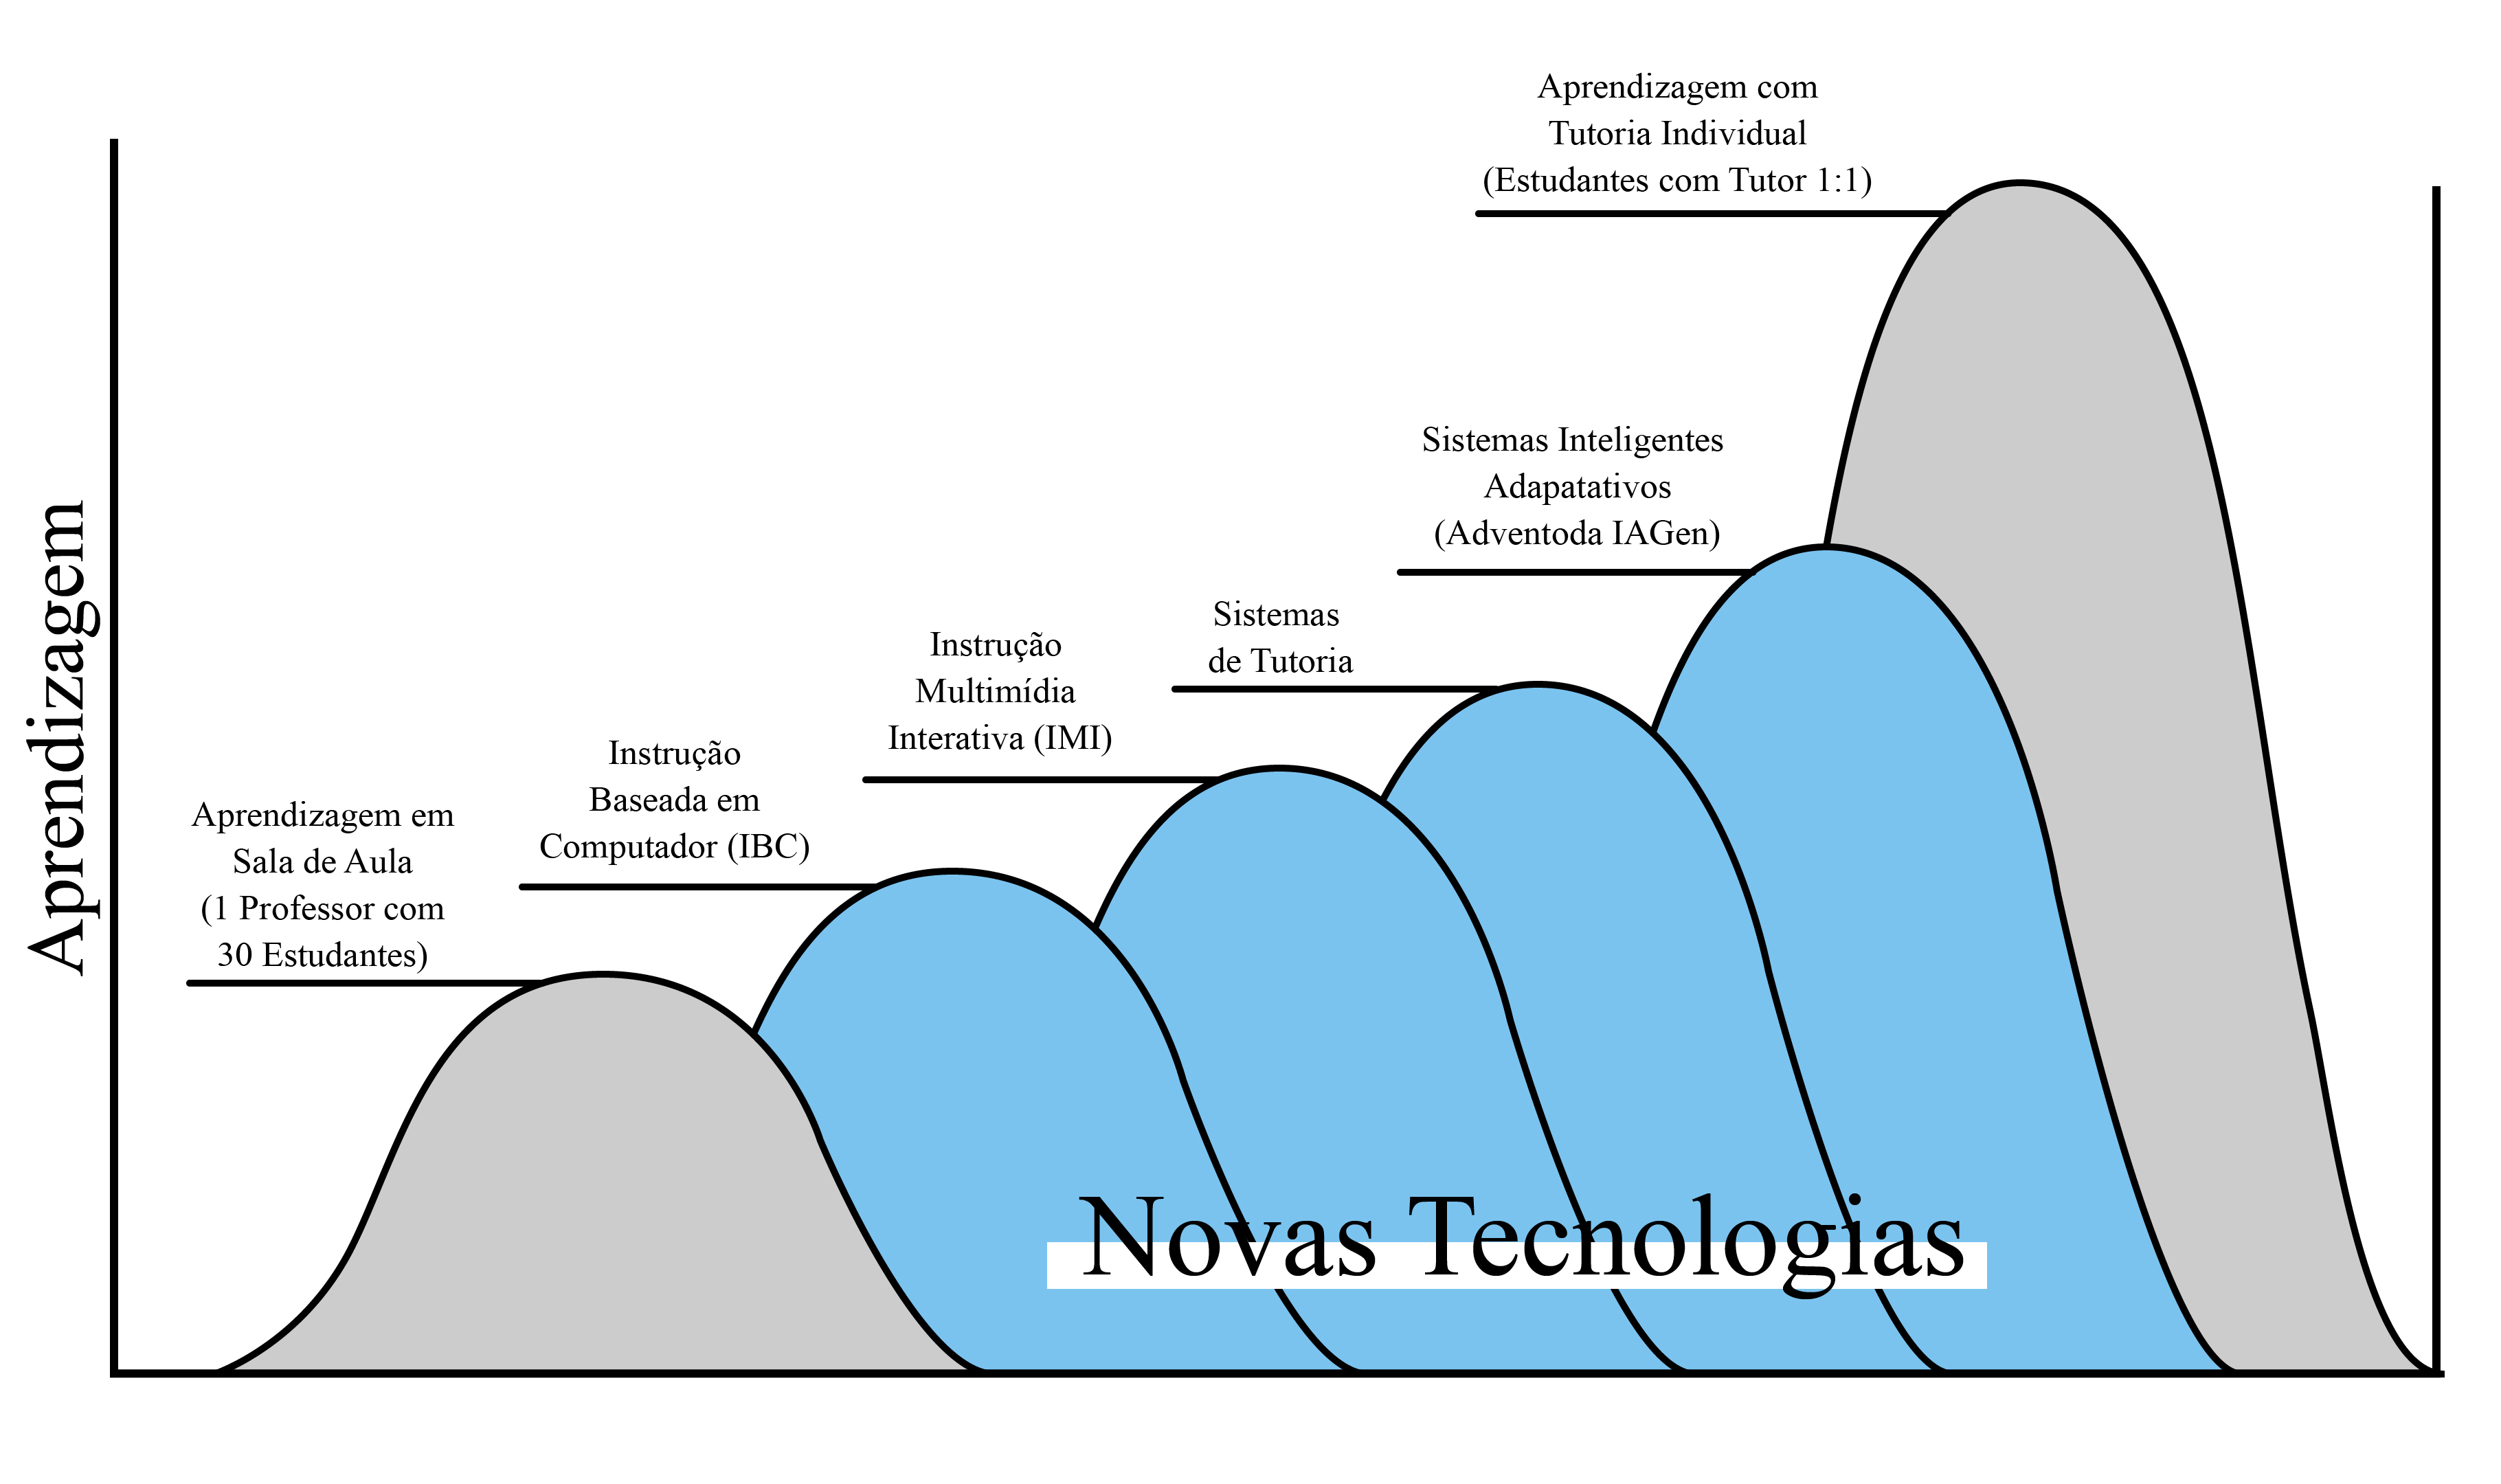
\includegraphics[width=1\textwidth]{images/chapter2-lo-engagement.jpg}
\fadaptada{Tarouco2021}
\end{figure}

Na próxima seção, exploraremos como o reconhecimento de fala pode promover a acessibilidade digital, abordando temas emergentes como IAGen, \sigla{NLP}{Processamento de Linguagem Natural} e \sigla{LLMs}{Grandes Modelos de Linguagem}. Através dessas tecnologias disruptivas, pretendemos potencializar ainda mais o alcance e a qualidade dos OAs nos mais diversos ambientes educacionais.

\section{Reconhecimento de Fala: Promovendo Acessibilidade Digital com IA}
\label{section:foundation:asr}

Na era digital, a educação está em constante evolução à medida que as tecnologias emergentes podem remodelar as abordagens pedagógicas tradicionais. Neste contexto, o ASR, interpretado neste trabalho como um sinônimo de STT, emerge como uma ferramenta poderosa. 

O conceito de ASR não apenas pode potencializar a acessibilidade de conteúdos com transcrições e legendas, mas também representa um passo significativo em direção a uma educação mais inclusiva. Nesse sentido, concordamos com \citeonline{Homburg2019} sobre o potencial do ASR nas TAs para surdos, dentre as quais destacamos os avatares de línguas de sinais baseados em texto em nosso MS \cite{FalvoJr2020_FIE, FalvoJr2020_SBIE, FalvoJr2021_RENOTE}.

Segundo \citeonline{fleischmann2021}, a ascensão do ensino remoto, acelerada por circunstâncias como a pandemia da COVID-19, impulsionou a busca por métodos inovadores para a criação e compartilhamento de conteúdos educacionais. Nessa conjuntura, o ASR se consolidou como uma ferramenta promissora, particularmente em ambientes colaborativos ou conferências online.

Desta forma, soluções baseadas em ASR desempenham um papel vital ao quebrar barreiras linguísticas, otimizando a comunicação entre falantes de diferentes línguas. Este argumento é reforçado por \citeonline{Homburg2019}, que destaca a relevância da tradução de voz para línguas de sinais visando promover a inclusão da comunidade surda no processo de ensino-aprendizagem.

Apesar de seu potencial, o ASR enfrenta diversos obstáculos e desafios de pesquisa. O trabalho de \citeonline{Koenecke2020} destaca alguns deles, apontando para disparidades raciais e as sutilezas de características linguísticas, como sotaques e peculiaridades regionais, assim como identificamos em nosso MS para a Libras. Essas constatações reforçam a relevância de promover soluções baseadas em ASR que sejam verdadeiramente inclusivas e que contemplem um espectro mais amplo de considerações sociolinguísticas em seu projeto e implementação.

\citeonline{Mayer2021} afirmam que o uso de tecnologias disruptivas, como o ASR, é fundamental para ampliar o alcance dos OAs a uma diversidade maior de aprendizes, promovendo conteúdos educacionais mais acessíveis. Na prática, \citeonline{Parakh2022} descreve OAs como unidades digitais reutilizáveis que muitas vezes são integradas em iniciativas \textit{open-source}, desempenhando um papel crucial ao moldar experiências de ensino-aprendizagem adaptáveis, democráticas e contextualizadas.

Estas recentes perspectivas reforçam e expandem nossas percepções obtidas em nosso MS, que enfatizou a importância das inovações tecnológicas no processo de ensino e aprendizagem de línguas de sinais, revelando gaps interessantes. Nesse sentido, notamos a falta de padrões de projeto, além de boas práticas de código e reuso, o que compromete a qualidade, o compartilhamento e o potencial de impacto desses OAs. 

Diante destas lacunas e das tendências emergentes citadas, projetamos a Arquitetura \textit{Speech2Learning}. Uma abstração que propõe diretrizes de desenvolvimento para a criação de soluções \textit{ASR-based}, promovendo maior acessibilidade de seus OAs, em especial os audíveis.

A evolução e sofisticação do ASR estão intimamente ligadas aos avanços em \sigla{ML}{\textit{Machine Learning}} e IA. A aplicação de modelos de ML em ASR permite a otimização contínua e a adaptação a diferentes contextos linguísticos e acústicos. Isso é alcançado através de técnicas de treinamento supervisionado e não supervisionado, utilizando vastas quantidades de dados de fala para melhorar a precisão e a robustez dos sistemas de reconhecimento.

O fluxo de processamento de fala em sistemas ASR é ilustrado na \autoref{figure:chapter2-asr-diagram}. O processo começa com a captura do sinal de fala, que é submetido a uma etapa de pré-processamento. Nessa fase, o sinal é filtrado para remover ruídos e normalizado para padrões específicos. Em seguida, ocorre a extração de características, onde as propriedades acústicas relevantes da fala são convertidas em vetores de características. Esses vetores representam os componentes principais da fala que serão utilizados nas próximas etapas.

\begin{figure}[htb]
\centering
\caption{Fluxo do Processamento de Fala em Sistemas ASR}
\label{figure:chapter2-asr-diagram}
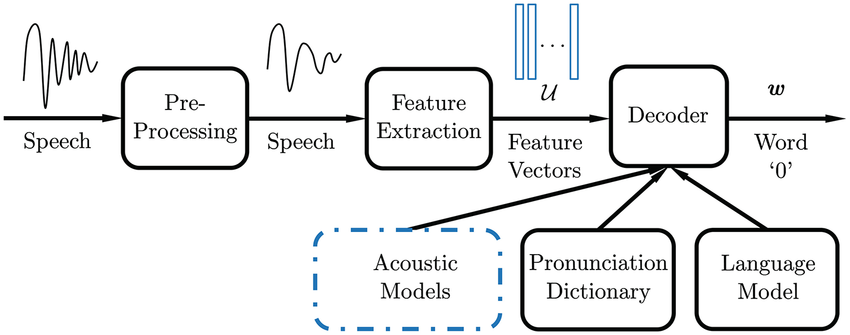
\includegraphics[width=0.9\textwidth]{images/chapter2-asr-diagram.png}
\fadaptada{Li2018}
\end{figure}

Após a extração de características, os vetores resultantes são alimentados em um decodificador. O decodificador utiliza modelos acústicos, um dicionário de pronúncia e um modelo de linguagem para interpretar os vetores de características e mapear palavras/frases correspondentes. Os modelos acústicos são responsáveis por capturar as nuances dos sons da fala, enquanto o dicionário de pronúncia fornece a correspondência entre as sequências de fonemas e palavras. 

O modelo de linguagem, que pode ser um LLM, ajuda a prever a sequência mais provável de palavras com base no contexto linguístico. Esta abordagem estruturada e baseada em modelos de ML e IA permite que sistemas de ASR sejam precisos e adaptáveis a uma ampla gama de variabilidades na fala humana.

A distinção entre ASR e STT é muitas vezes sutil e pode ser usada de forma intercambiável, como optamos neste trabalho para simplificação. Enquanto ASR geralmente refere-se ao campo de estudo e tecnologia de reconhecimento automático de fala, STT descreve a função específica de converter fala em texto. Ambos os termos são fundamentais para o desenvolvimento de tecnologias de acessibilidade e têm aplicações que se sobrepõem consideravelmente.

Em resumo, o reconhecimento de fala, através do uso de tecnologias como ASR e STT, suportado por avanços em ML e IA, tem um potencial transformador para promover a acessibilidade digital. Estas tecnologias não só facilitam a criação de conteúdos mais inclusivos, mas também permitem a adaptação e personalização da educação para atender às necessidades de uma diversidade maior de aprendizes. Assim, a integração de ASR representa um marco significativo na trajetória para uma educação mais acessível.

\section{Considerações Finais}

As análises e discussões apresentadas nesta fundamentação teórica permitiram uma compreensão abrangente das interseções entre TICs e línguas de sinais no contexto educacional. O MS realizado, detalhado na \autoref{section:foundation:sm}, revelou importantes lacunas tecnológicas e de pesquisa na utilização de línguas de sinais para o ensino-aprendizagem, destacando áreas onde inovações são urgentemente necessárias. Esses gaps tecnológicos foram essenciais para orientar a condução de um levantamento bibliográfico adicional, visando identificar e explorar TICs promissoras que pudessem mitigar os desafios identificados e promover uma educação mais inclusiva.

No decorrer desta fundamentação teórica, exploramos de forma aprofundada diversos aspectos cruciais, incluindo Arquiteturas de Software, OAs e ASR. A \autoref{section:foundation:arch} discute arquiteturas de software inovadoras que suportam a integração eficiente de TICs no processo educacional, enquanto a \autoref{section:foundation:lo} foca nos OAs, destacando sua importância na criação de materiais educacionais adaptáveis e acessíveis. Particularmente, a \autoref{section:foundation:asr} demonstrou como as tecnologias de ASR podem ser aplicadas para melhorar a acessibilidade de conteúdos educacionais, proporcionando uma base teórica robusta para a arquitetura \textit{Speech2Learning}.

Através da síntese destas temáticas, esta fundamentação teórica estabelece os alicerces para a proposição da \textit{Speech2Learning}, uma arquitetura inovadora que visa tornar os Objetos de Aprendizagem audíveis mais acessíveis. Definida em detalhes no \autoref{chapter3}, a \textit{Speech2Learning} representa uma proposta baseada no uso de ASR para educação inclusiva, aproveitando as últimas inovações em TICs e IA para criar soluções educacionais que atendam às necessidades de uma diversidade maior de aprendizes. Esta fundamentação teórica, portanto, não apenas ilumina as lacunas existentes, mas também propõe caminhos concretos para superá-las, contribuindo para o avanço da pesquisa e prática educacional inclusiva.

\chapter{Arquitetura Speech2Learning: Potencializando a Acessibilidade em Objetos de Aprendizagem com Reconhecimento de Fala}
\label{chapter3}
\section{Considerações Iniciais}

A arquitetura \textit{Speech2Learning} foi motivada por um MS prévio, detalhado na \autoref{section:foundation:sm}, cujo objetivo foi identificar o papel da tecnologia no ensino e aprendizagem, particularmente através das línguas de sinais \cite{FalvoJr2020_SBIE, FalvoJr2020_FIE, FalvoJr2021_RENOTE}. Este estudo proporcionou uma visão abrangente sobre o uso das TICs para o desenvolvimento de TA, evidenciando a importância significativa de novas tecnologias para um processo de ensino-aprendizagem mais inclusivo.

Contudo, foi observada uma lacuna importante: a ausência de padrões e boas práticas de desenvolvimento que facilitassem o compartilhamento e reuso de OAs. Como resposta a essa necessidade, a arquitetura \textit{Speech2Learning} foi estabelecida para promover a criação de soluções estruturalmente preparadas para a inclusão, não apenas de pessoas surdas, mas também de aprendizes que necessitam de maior acessibilidade em conteúdos educacionais audíveis \cite{FalvoJr2023_HICSS}.

Além disso, a \textit{Speech2Learning} adota uma abordagem modular e escalável, permitindo que diferentes componentes de reconhecimento de fala e processamento de áudio sejam integrados de forma flexível. Isso possibilita que a arquitetura se adapte a diversos contextos educacionais e necessidades específicas dos aprendizes. A arquitetura também enfatiza a interoperabilidade e a conformidade com padrões abertos, facilitando a integração com outras plataformas e ferramentas educacionais, promovendo um ecossistema mais colaborativo e acessível.

A evolução da área de IA, especialmente com modelos generativos, tem o potencial de expandir ainda mais as capacidades da \textit{Speech2Learning}. A IAGen, com a habilidade de processar e gerar texto de forma autônoma, pode ser utilizada para aprimorar a acessibilidade e a personalização dos OAs, abrindo novas possibilidades para a criação de conteúdo e interação com os alunos.

Nesse sentido, a \textit{Speech2Learning} não apenas aborda a lacuna identificada em relação à falta de padrões, mas também estabelece um \textit{framework} robusto e inclusivo para o desenvolvimento de soluções educacionais baseadas em reconhecimento automático de fala. A arquitetura visa transformar a maneira como os conteúdos educacionais audíveis são criados e acessados, promovendo uma educação mais inclusiva e acessível para todos os aprendizes.

\section{Principais Referências e Inspirações}

Tecnicamente, a \textit{Speech2Learning} propõe um arcabouço genérico que vai além das línguas de sinais, escopo inicial do MS conduzido neste trabalho \cite{FalvoJr2020_SBIE, FalvoJr2020_FIE, FalvoJr2021_RENOTE}. No entanto, ele fornece uma abstração que facilita a acessibilidade de OAs audíveis, permitindo a geração de transcrições e, consequentemente, a sinalização do conteúdo educacional em questão. Nesse contexto, soluções baseadas em avatares, tais como \textit{Hand Talk} ou \textit{VLibras}, podem ser utilizadas com base nas transcrições, tornando os conteúdos acessíveis para usuários das línguas de sinais.

Sendo assim, foi proposta a arquitetura \textit{Speech2Learning}, uma adaptação da \textit{Clean Architecture} de \citeonline{martin2017}, com o objetivo específico de promover a acessibilidade de OAs por meio do reconhecimento de fala. Segundo \citeonline{martin2017}, a \textit{Clean Architecture} é uma ideia prática que integra algumas das principais referências em ES nas últimas décadas \cite{cockburn2005, freeman2009, palermo2008, coplien2012, reenskaug2009, jacobson1992}. 

Essas iniciativas compartilham a ideia central de separar o código em camadas independentes, com o domínio no núcleo da arquitetura. Isso permite a criação de sistemas altamente testáveis, independentes de tecnologia, e adaptáveis às necessidades específicas de um projeto. A arquitetura \textit{Speech2Learning}, alinhada a esses princípios, concentra seu domínio de aplicação central nos OAs, conforme representado pela \autoref{fig:chapter3-speech2learning-arch}. 

\begin{figure}[htb]
\centering
\caption{arquitetura \textit{Speech2Learning}}
\label{fig:chapter3-speech2learning-arch}
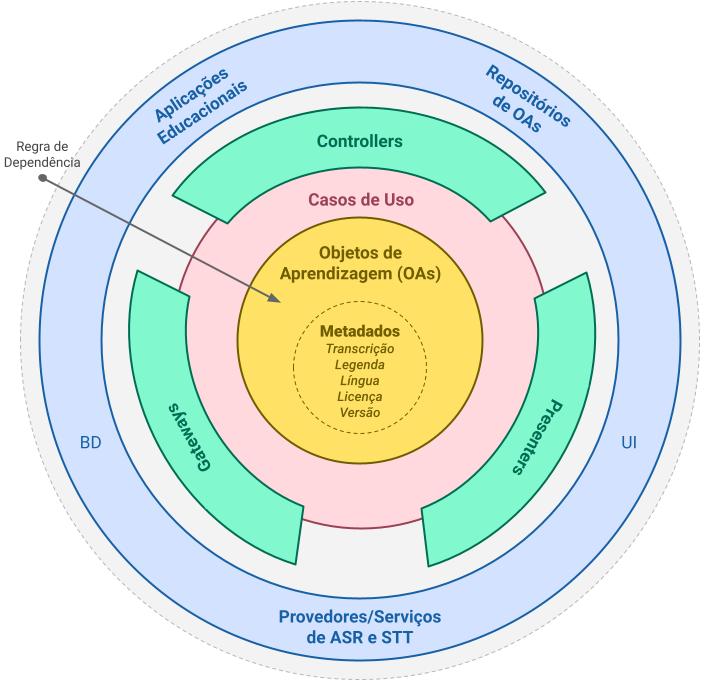
\includegraphics[width=0.71\textwidth]{images/chapter3-speech2learning-arch.png}
\fadaptada{FalvoJr2023_HICSS}
\end{figure}

Cada camada da \textit{Speech2Learning} contribui de forma significativa para OAs mais acessíveis por meio dos conceitos de ASR/STT, os quais, em conjunto com os metadados, são cruciais para promover a acessibilidade dos OAs de forma padronizada e consistente. Vale ressaltar que uma arquitetura não tem como objetivo definir detalhes de implementação, mas sim abstrações de software que podem ser adaptadas de acordo com as necessidades de cada domínio de aplicação. A seguir, apresenta-se uma síntese de cada uma das camadas definidas pela arquitetura:

\begin{itemize}
\item \textbf{Objetos de Aprendizagem (Amarelo)}: Responsável pelos modelos e regras de negócio do domínio. Para garantir que os OAs sejam mais acessíveis e padronizados, as entidades podem incluir transcrição, legendagem e outras capacidades compatíveis com o domínio de aplicação e o padrão de metadados dos OAs audíveis. Além disso, o processo de reconhecimento de fala deve ser, idealmente, multimodal (abrangendo áudio e vídeo) e suportar múltiplos idiomas. Nesse sentido, considerar IAs, especialmente as generativas, é recomendado uma vez que elas resolvem de forma efetiva muitos desses desafios técnicos. Sendo assim, desde o centro da nossa arquitetura, onde estão os OAs, se faz necessária uma visão de projeto arquitetural que tenha sinergia com IAGen;
\item \textbf{Casos de Uso (Vermelho)}: Operações de alto nível e regras de negócio do sistema. Em outras palavras, esta camada é responsável por orquestrar as regras encapsuladas nos OAs, função comumente chamada de ``dança das entidades'';
\item \textbf{Adaptadores (Verde)}: Tem a responsabilidade de converter os dados para um formato conveniente, considerando as necessidades das camadas com as quais faz fronteira;
\item \textbf{Infraestrutura (Azul)}: Abrange questões técnicas e específicas, como \textit{frameworks}, \textit{drivers} e integrações externas. Nesse sentido, conexões com \sigla{BDs}{Bancos de Dados}, serviços de ASR/STT ou eventuais integrações com APIs de IAGen fariam parte desta camada. Além disso, ela inclui a \sigla{UI}{Interface do Usuário}, abrangendo a conexão com aplicações educacionais concretas (\textit{d-learning}, \textit{e-learning}, \textit{m-learning} etc) ou repositórios de OAs;
\item \textbf{Principal e Configuração (Cinza)}: Estabelece todas as conexões entre interfaces e suas implementações concretas, além de ser responsável por configurar e executar a aplicação.
\end{itemize}

A ``Regra de Dependência'' define que as dependências de código devem apontar apenas para dentro, em direção aos OAs, nunca para fora. Desse modo, a \textit{Speech2Learning} favorece a adaptabilidade, independência tecnológica e testabilidade, fornecendo uma orientação estrutural para a criação de soluções educacionais mais acessíveis. 

Portanto, é fundamental que as responsabilidades e boas práticas de suas camadas sejam bem compreendidas, pois elas estruturam diretrizes de projeto genéricas para a criação de soluções de TA baseadas em ASR. As seções a seguir detalham cada uma dessas camadas.

\section{Camada de Entidades (Objetos de Aprendizagem)}

\begin{figure}[htb]
\centering
\caption{Camada de Entidades (Objetos de Aprendizagem)}
\label{fig:chapter3-speech2learning-layer1}
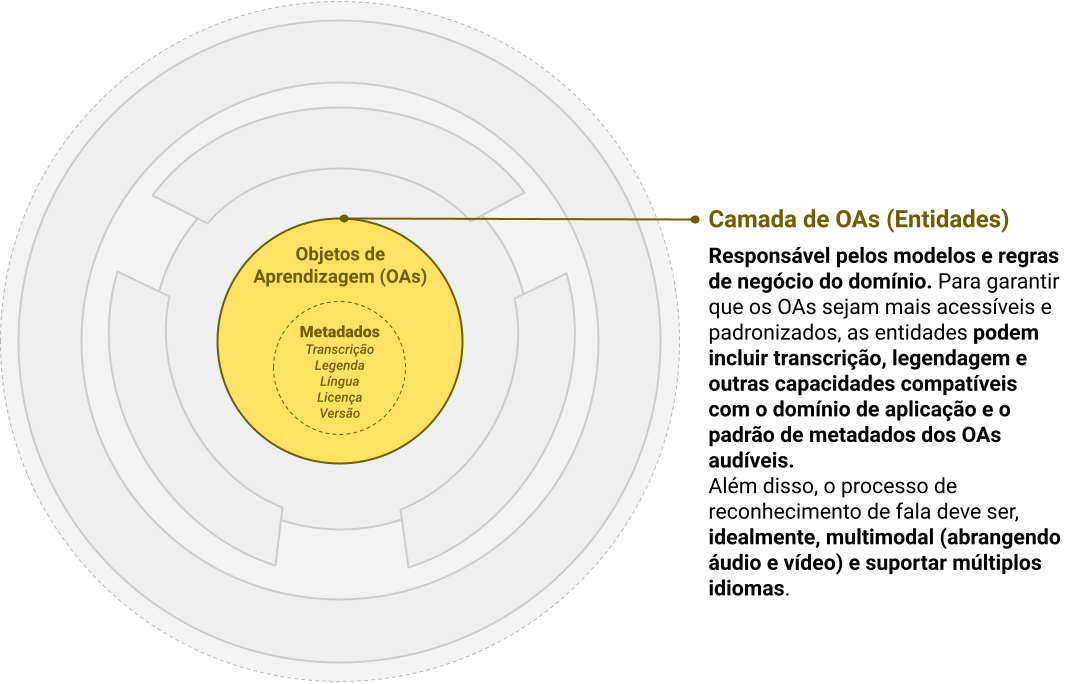
\includegraphics[width=1\textwidth]{images/chapter3-speech2learning-layer1.png}
\fadaptada{FalvoJr2023_HICSS,Lemos2022}
\end{figure}

A Camada de Entidades na arquitetura \textit{Speech2Learning} é central para a definição dos modelos e regras de negócio do domínio dos OAs (\autoref{fig:chapter3-speech2learning-layer1}). Esta camada é responsável por encapsular os dados fundamentais e as lógicas que regem a estrutura e o comportamento dos OAs, garantindo sua acessibilidade e padronização. 

Para alcançar esses objetivos, é crucial incorporar padrões de metadados estabelecidos, como Dublin Core, SCORM, MISB, LOM e RDF, que fornecem diretrizes consistentes para a definição e organização dos conteúdos educacionais \cite{Santana2023}. As principais responsabilidades da Camada de Entidades incluem:

\begin{itemize}
    \item \textbf{Modelagem dos OAs}: Definir e estruturar os OAs de forma a garantir sua acessibilidade. Isso inclui a inclusão de elementos como transcrição, legendagem e outros recursos que tornam os conteúdos audíveis acessíveis a uma ampla gama de aprendizes, incluindo aqueles com necessidades especiais.

    \item \textbf{Definição de Regras de Negócio do Domínio}: Estabelecer regras de negócio que governam o comportamento dos OAs, assegurando que os processos de ensino-aprendizagem sejam eficazes e inclusivos. As regras de negócio devem considerar a multimodalidade do reconhecimento de fala, abrangendo áudio e vídeo, e suportando múltiplos idiomas.

    \item \textbf{Padronização e Interoperabilidade}: Garantir que os OAs sejam compatíveis com os padrões de metadados, facilitando seu compartilhamento e reuso em diferentes plataformas educacionais. A conformidade com padrões como Dublin Core, SCORM, MISB, LOM e RDF é essencial para manter a consistência e a qualidade dos OAs.
\end{itemize}

Os padrões de metadados desempenham um papel crucial na definição e organização dos OAs. A seguir, ilustra-se como cada padrão pode ser aplicado na Camada de OAs (Entidades):

\begin{itemize}
    \item \textbf{Dublin Core}: Fornece um conjunto simples e genérico de elementos para descrever recursos digitais. Na Camada de Entidades, Dublin Core pode ser utilizado para definir metadados básicos como título, autor, descrição, data, formato e identificador dos OAs, facilitando sua catalogação e recuperação.

    \item \textbf{SCORM}: É um padrão para LMS que facilita o reuso de conteúdos educacionais. Na \textit{Speech2Learning}, SCORM pode ser utilizado para definir a estrutura modular dos OAs, permitindo que cada unidade de aprendizagem seja facilmente reutilizada e integrada em diferentes cursos e plataformas.

    \item \textbf{MISB}: Embora mais comum em contextos de vídeo e imagem em movimento, MISB pode ser aplicado para garantir que os conteúdos audiovisuais dos OAs sejam padronizados e interoperáveis, especialmente em termos de metadados de vídeo e áudio.

    \item \textbf{LOM}: É um padrão específico para descrever OAs. Na Camada de Entidades, LOM pode ser utilizado para definir metadados detalhados que incluem, além dos elementos básicos, informações pedagógicas como tipo de recurso, nível de dificuldade, tempo de aprendizagem e público-alvo.

    \item \textbf{RDF}: Facilita a interoperabilidade de dados na web. Na \textit{Speech2Learning}, RDF pode ser utilizado para criar descrições estruturadas e semânticas dos OAs, permitindo que os dados sobre os objetos sejam facilmente compartilhados e integrados com outros sistemas e plataformas educacionais.
\end{itemize}

Do ponto de vista prático, o \autoref{codigo:exemplo-camada1} exemplifica o modelo \textit{TranscribedAudio}, o qual estabelece uma conexão com as responsabilidades citadas. Além disso, elementos fundamentais como documentação, convenções e boas práticas se mostram presentes. Outro aspecto fundamental é a independência de \textit{frameworks} e bibliotecas, caracterizando uma entidade limpa.

\begin{codigo}[caption={Exemplo Camada de Entidades: Disponível em \url{https://bit.ly/S2L-Entity}}, label={codigo:exemplo-camada1}, language=Java, breaklines=true]
/**
 * Model that represents an audio file and its transcript.
 * Responsibilities:
 * - Hold properties: ID, name, content, transcript.
 * - Validate integrity and conformity of audio data.
 * Adherence to Clean Architecture:
 * - Central to business logic and rules.
 * - Independent of frameworks or data persistence.
 * 
 * Author: @falvojr
 */
public class TranscribedAudio {
  private String id, name, transcript;
  private InputStream content;

  public void validate() {
    if (empty(name) || empty(transcript) || empty(content)) {
      String msg =  "Name, transcript and content required.";
      throw new EnterpriseBusinessException(msg);
    }
    String ext = FileUtils.getExtension(name).toLowerCase();
    if (!VALID_EXT.contains(ext)) {
      String msg =  "Invalid ext, use %s".formatted(VALID_EXT);
      throw new EnterpriseBusinessException(msg);
    }
  }
}
\end{codigo}

Por fim, para garantir maior acessibilidade e internacionalização dos OAs, é essencial que esta camada considere o ASR de forma multimodal, abrangendo tanto áudio quanto vídeo. Isso permite que os conteúdos educacionais audíveis sejam mais diversos e flexíveis às diferentes necessidades dos aprendizes. Além disso, a capacidade de suportar múltiplos idiomas é fundamental para a inclusão de aprendizes de diversas origens linguísticas, promovendo uma educação verdadeiramente inclusiva e global.

Adicionalmente, a IAGen pode ser utilizada para enriquecer os metadados dos OAs, gerando automaticamente descrições mais detalhadas e informativas, \textit{tags} relevantes e até mesmo traduções para diferentes idiomas, aumentando a descoberta e a reutilização dos OAs em diferentes contextos e por diferentes públicos.

\section{Camada de Aplicação (Casos de Uso)}

\begin{figure}[htb]
\centering
\caption{Camada de Aplicação (Casos de Uso)}
\label{fig:chapter3-speech2learning-layer2}
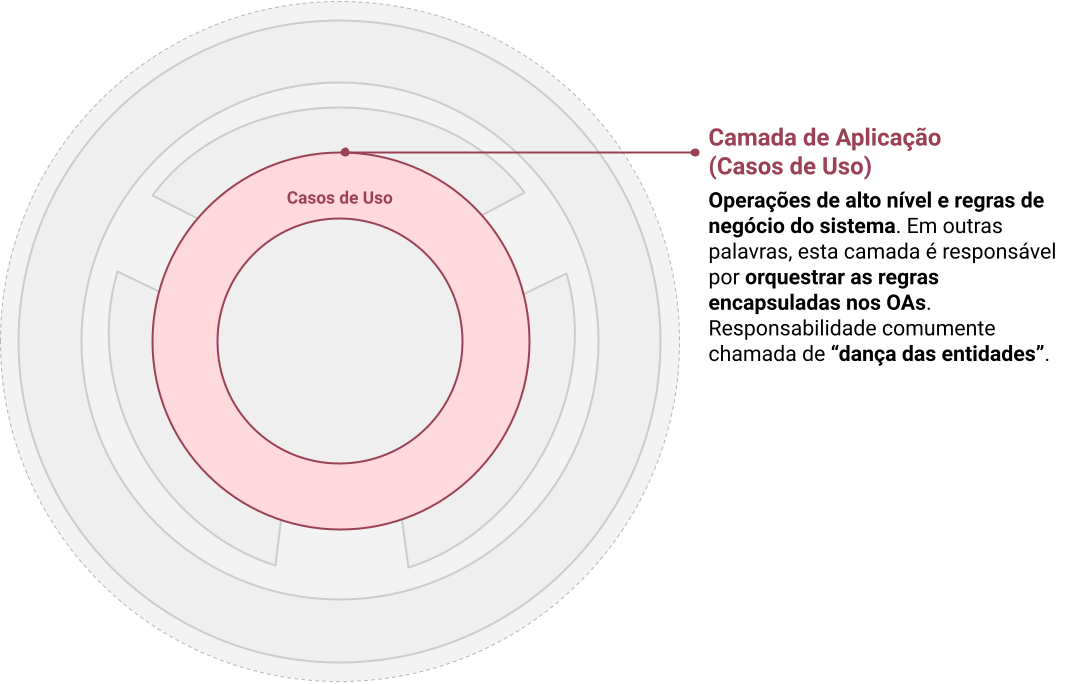
\includegraphics[width=.98\textwidth]{images/chapter3-speech2learning-layer2.png}
\fadaptada{FalvoJr2023_HICSS, Lemos2022}
\end{figure}

A Camada de Aplicação na arquitetura \textit{Speech2Learning} é responsável pela implementação das regras de negócio da aplicação, ou seja, dos casos de uso. Esta camada orquestra as operações de alto nível, garantindo que as regras encapsuladas nos OAs sejam executadas de maneira eficiente e coerente com os objetivos educacionais e de acessibilidade da arquitetura (\autoref{fig:chapter3-speech2learning-layer2}). As principais responsabilidades da Camada de Aplicação incluem:

\begin{itemize}
    \item \textbf{Orquestração de Regras de Negócio}: Implementar e gerenciar as regras de negócio que definem o comportamento dos OAs, garantindo que as operações de ensino e aprendizagem sejam conduzidas de maneira consistente com os objetivos de acessibilidade e inclusão.

    \item \textbf{Coordenação de Fluxos de Trabalho}: Coordenar os diversos fluxos de trabalho relacionados aos processos de ensino-aprendizagem, incluindo a transcrição, legendagem e geração de metadados, assegurando que todas as etapas sejam integradas de forma harmoniosa.

    \item \textbf{Interação com Outras Camadas}: Facilitar a comunicação entre a Camada de Entidades e as externas (Adaptadores e Infraestrutura), garantindo que as operações sejam executadas corretamente e que os dados sejam processados/transmitidos conforme necessário.
\end{itemize}

Na prática, algumas abstrações são essenciais para a implementação eficaz dos casos de uso. Como sugestões de abstrações que fazem sentido para essa arquitetura destacam-se:

\begin{itemize}
    \item \textbf{Controladores de Casos de Uso}: Classes ou componentes que implementam casos de uso específicos, orquestrando as operações de acordo com as regras de negócio. Por exemplo, um controlador pode gerenciar o processo de transcrição de um conteúdo de áudio, interagindo com a Camada de Entidades para armazenar os resultados e atualizar os metadados do OA.

    \item \textbf{Serviços de Aplicação}: Componentes que encapsulam lógica de negócio reutilizável, fornecendo funcionalidades comuns a múltiplos casos de uso. Exemplos incluem serviços para processamento de áudio, reconhecimento de fala ou geração de legendas, que podem ser utilizados por diferentes controladores de casos de uso.

    \item \textbf{Repositórios de Casos de Uso}: Interfaces e implementações que gerenciam a persistência e recuperação de dados necessários para a execução dos casos de uso. Estes repositórios abstraem o acesso aos dados, permitindo que a lógica de negócio permaneça desacoplada das questões de persistência.

    \item \textbf{\sigla{DTO}{\textit{Data Transfer Objects}}}: Objetos de transferência de dados utilizados para encapsular e transportar dados entre as diferentes camadas da arquitetura. Os DTOs garantem que os dados sejam transmitidos de maneira eficiente e coerente, facilitando a comunicação entre controladores de casos de uso e outros componentes do sistema.

    \item \textbf{Interfaces de Serviços Externos}: Abstrações que representam serviços externos necessários para a execução dos casos de uso, como APIs de ASR, serviços de tradução ou plataformas de gestão de conteúdos educacionais. Estas interfaces permitem que a Camada de Aplicação interaja com serviços externos de maneira flexível e desacoplada.
\end{itemize}

Nesse contexto, tem-se como exemplo um caso de uso que orquestra o processo de transcrição de áudio para texto, interagindo com serviços de reconhecimento de fala e atualizando os metadados do OA para incluir a transcrição gerada. Essa implementação foi parte de uma das POCs realizadas ao longo deste trabalho de doutorado, discutida no \autoref{chapter4}, e está disponível neste repositório \textit{open-source}: \url{https://bit.ly/S2L-UseCase}.

Tais abstrações e exemplos demonstram como a Camada de Aplicação pode ser estruturada para orquestrar de forma eficiente os OAs aderentes aos princípios da \textit{Speech2Learning}, promovendo a acessibilidade por meio de soluções baseadas em reconhecimento de fala.

A IAGen pode também ser aplicada nesta camada para implementar casos de uso inovadores, como a geração automática de roteiros para videoaulas, a criação de \textit{chatbots} para interação com os aprendizes e a personalização do \textit{feedback} em atividades avaliativas.

\section{Camada de Adaptadores}

\begin{figure}[htb]
\centering
\caption{Camada de Adaptadores}
\label{fig:chapter3-speech2learning-layer3}
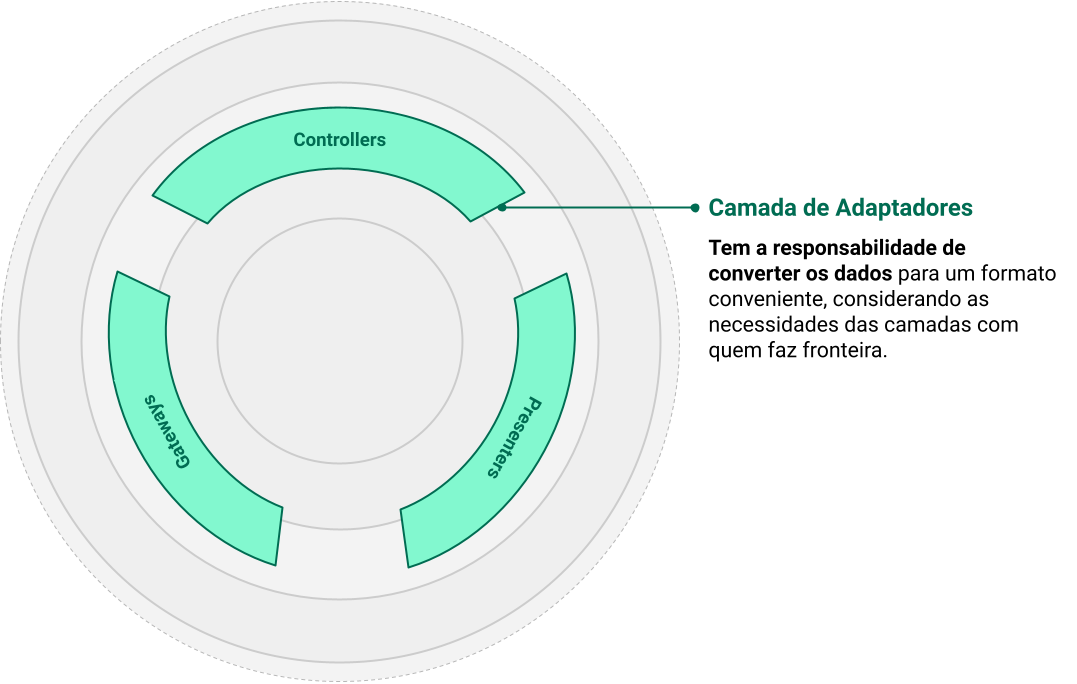
\includegraphics[width=.95\textwidth]{images/chapter3-speech2learning-layer3.png}
\fadaptada{FalvoJr2023_HICSS, Lemos2022}
\end{figure}

A Camada de Adaptadores na arquitetura \textit{Speech2Learning} tem a responsabilidade de converter os dados para um formato conveniente, considerando as necessidades das camadas com as quais faz fronteira. Esta camada atua como um intermediário crucial, garantindo que a comunicação entre as diferentes partes do sistema ocorra de maneira eficiente e coerente (\autoref{fig:chapter3-speech2learning-layer3}). As principais responsabilidades da Camada de Adaptadores incluem:

\begin{itemize}
    \item \textbf{Conversão de Dados}: Transformar os dados entre os formatos utilizados pelas camadas de Aplicação, Entidades e Infraestrutura, assegurando que cada camada receba os dados no formato mais adequado para sua funcionalidade.

    \item \textbf{Isolamento de Detalhes Técnicos}: Abstrair os detalhes técnicos de implementação, permitindo que as camadas superiores (Aplicação e Entidades) permaneçam independentes das preocupações técnicas específicas de integração com sistemas externos e infraestrutura.

    \item \textbf{Facilitação da Comunicação}: Garantir que a comunicação entre as diferentes camadas do sistema seja transparente e eficiente, minimizando os impactos de mudanças em uma camada sobre as demais.
\end{itemize}

Na \textit{Speech2Learning}, algumas abstrações são essenciais para a implementação eficaz dos adaptadores. Como sugestões de abstrações que fazem sentido para essa arquitetura destacam-se:

\begin{itemize}
    \item \textbf{Adaptadores de Entrada}: Componentes responsáveis por receber dados de fontes externas (como APIs, BDs ou UI) e convertê-los para um formato que possa ser processado pela Camada de Aplicação. Por exemplo, um adaptador de entrada pode receber dados de áudio de uma API de ASR e convertê-los em texto para processamento posterior.

    \item \textbf{Adaptadores de Saída}: Componentes que transformam dados gerados pela Camada de Aplicação em um formato que pode ser utilizado por sistemas externos ou armazenado em BDs. Por exemplo, um adaptador de saída pode transformar transcrições de texto em um formato adequado para armazenamento em um ROAs.

    \item \textbf{Interfaces de Conversão de Dados}: Abstrações que definem métodos para converter dados entre diferentes formatos e protocolos. Estas interfaces garantem que a lógica de conversão seja desacoplada das implementações específicas, promovendo reutilização e facilidade de manutenção.

    \item \textbf{Serviços de Mapeamento de Dados}: Componentes responsáveis por mapear diferentes estruturas de dados, simplificando a conversão de objetos complexos e a integração com sistemas variados. Por exemplo, um serviço pode converter objetos de uma linguagem de programação específica em metadados compatíveis com padrões como SCORM ou LOM.
\end{itemize}

Para ilustrar a aplicação das abstrações sugeridas, considere um exemplo de um adaptador de entrada que implementa um cliente HTTP, como o \textit{Open Feign}, para interagir com um serviço externo de transcrição, especificamente a API da OpenAI. Este adaptador recebe dados de áudio, converte-os para um formato adequado para a API, e traduz as respostas da API para um formato compreensível pelo domínio. 

Essa implementação foi desenvolvida em colaboração com a DIO e está disponível neste repositório \textit{open-source}: \url{https://bit.ly/S2L-Adapters}. Tais abstrações e exemplos demonstram como a Camada de Adaptadores pode ser estruturada para garantir a conversão eficiente de dados entre diferentes partes do sistema \textit{Speech2Learning}, promovendo a interoperabilidade e a flexibilidade necessárias para uma solução educacional baseada em reconhecimento de fala.

Adicionalmente, a IAGen pode ser integrada aos adaptadores para realizar tarefas como a tradução automática de legendas, a geração de descrições de áudio para pessoas com deficiência visual e a conversão de formatos de dados complexos em formatos mais simples e acessíveis.

\section{Camada de Infraestrutura}

\begin{figure}[htb]
\centering
\caption{Camada de Infraestrutura}
\label{fig:chapter3-speech2learning-layer4}
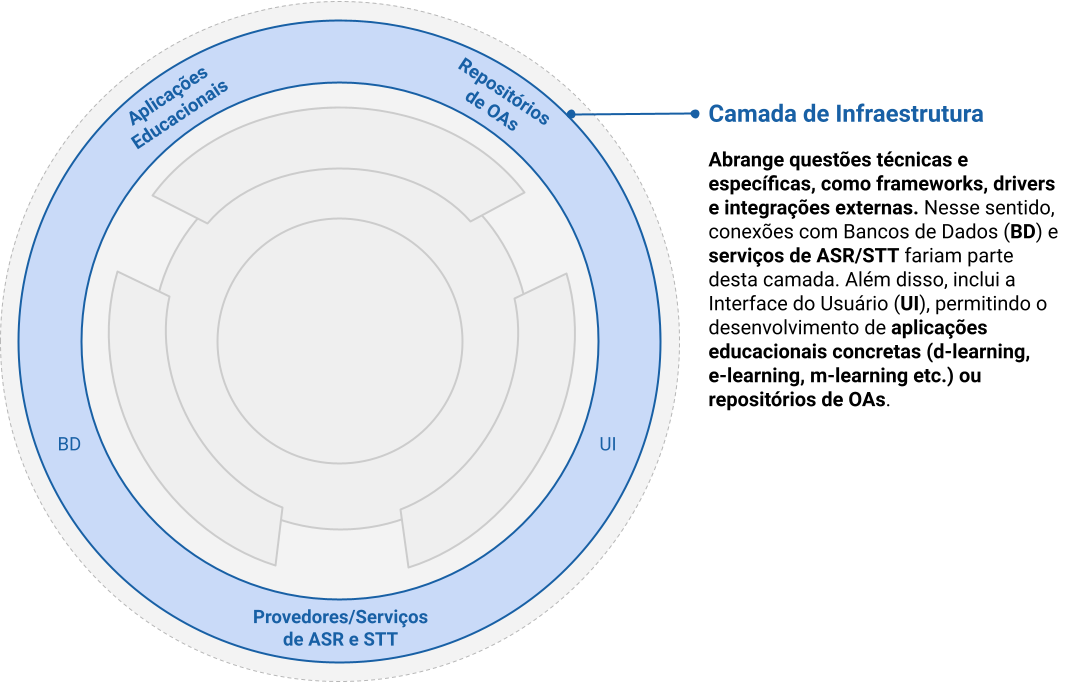
\includegraphics[width=1\textwidth]{images/chapter3-speech2learning-layer4.png}
\fadaptada{FalvoJr2023_HICSS, Lemos2022}
\end{figure}

A Camada de Infraestrutura na arquitetura \textit{Speech2Learning} abrange questões técnicas e específicas, como \textit{frameworks}, \textit{drivers} e integrações externas. Nesse sentido, conexões com BDs e serviços de ASR/STT fazem parte desta camada. Além disso, inclui a Interface do Usuário (UI), permitindo o desenvolvimento de aplicações educacionais concretas (\textit{d-learning}, \textit{e-learning}, \textit{m-learning}, etc) ou repositórios de OAs (\autoref{fig:chapter3-speech2learning-layer4}). As principais responsabilidades da Camada de Infraestrutura incluem:

\begin{itemize}
    \item \textbf{Gerenciamento de Dados}: Conectar e interagir com sistemas de gerenciamento de BDs para armazenar, recuperar e manipular os dados necessários para a aplicação, garantindo que os dados sejam acessíveis e seguros.

    \item \textbf{Integrações Externas}: Gerenciar a comunicação com serviços externos, como APIs de reconhecimento de fala e serviços de tradução, garantindo que a aplicação possa utilizar funcionalidades fornecidas por terceiros.

    \item \textbf{Suporte a UI}: Fornecer a infraestrutura necessária para o desenvolvimento e operação das interfaces de usuário, permitindo que os aprendizes interajam com os OAs de maneira eficaz e intuitiva.

    \item \textbf{Manutenção de Infraestrutura Técnica}: Gerenciar componentes técnicos, incluindo \textit{drivers}, bibliotecas e \textit{frameworks}, que são essenciais para o funcionamento da aplicação, assegurando que todos os elementos estejam atualizados e funcionando corretamente.
\end{itemize}

Para a \textit{Speech2Learning}, algumas abstrações são essenciais para a implementação eficaz da infraestrutura. Entre as sugestões de abstrações que fazem sentido para essa arquitetura tem-se:

\begin{itemize}
    \item \textbf{Repositórios de Dados}: Interfaces e implementações responsáveis por gerenciar a persistência dos dados, encapsulando a lógica de acesso ao BD e garantindo a independência da Camada de Aplicação em relação às tecnologias de armazenamento.

    \item \textbf{Serviços de Integração}: Componentes que facilitam a comunicação com serviços externos, fornecendo interfaces padronizadas para interagir com APIs de reconhecimento de fala, serviços de tradução e outras ferramentas externas.

    \item \textbf{Gerenciadores de UI}: Abstrações que suportam o desenvolvimento e a operação das interfaces de usuário, assegurando que a experiência do usuário seja consistente e acessível.

    \item \textbf{\textit{Drivers} e Bibliotecas}: Componentes técnicos que fornecem funcionalidades específicas necessárias para a operação da aplicação, como \textit{drivers} de BDs, bibliotecas de manipulação de áudio e ferramentas de desenvolvimento de UI.
\end{itemize}

Para que se tenha uma perspectiva prática, segue um exemplo de um adaptador que implementa a persistência de dados de áudio transcritos utilizando o \textit{MongoDB} e seu sistema de arquivos \textit{GridFS}. Este adaptador lida com operações de \sigla{CRUD}{\textit{Create, Read, Update and Delete}} para entidades de áudio transcritas, gerenciando o armazenamento de conteúdo e metadados de maneira eficiente. Essa implementação está disponível no seguinte repositório \textit{open-source}: \url{https://bit.ly/S2L-Infra}.

Essas abstrações e exemplos demonstram como a Camada de Infraestrutura pode ser estruturada para fornecer o suporte técnico necessário para a arquitetura \textit{Speech2Learning}, garantindo a interoperabilidade e a eficiência das operações de armazenamento e integração com serviços externos. Além disso, a IAGen pode ser utilizada para otimizar o desempenho da infraestrutura, por meio da análise de dados de uso e da identificação de padrões que permitam a alocação eficiente de recursos e a melhoria da escalabilidade do sistema.

\section{Pseudo-camada ``Principal \& Configuração''}

\begin{figure}[htb]
\centering
\caption{Pseudo-camada Principal \& Configuração}
\label{fig:chapter3-speech2learning-layer5}
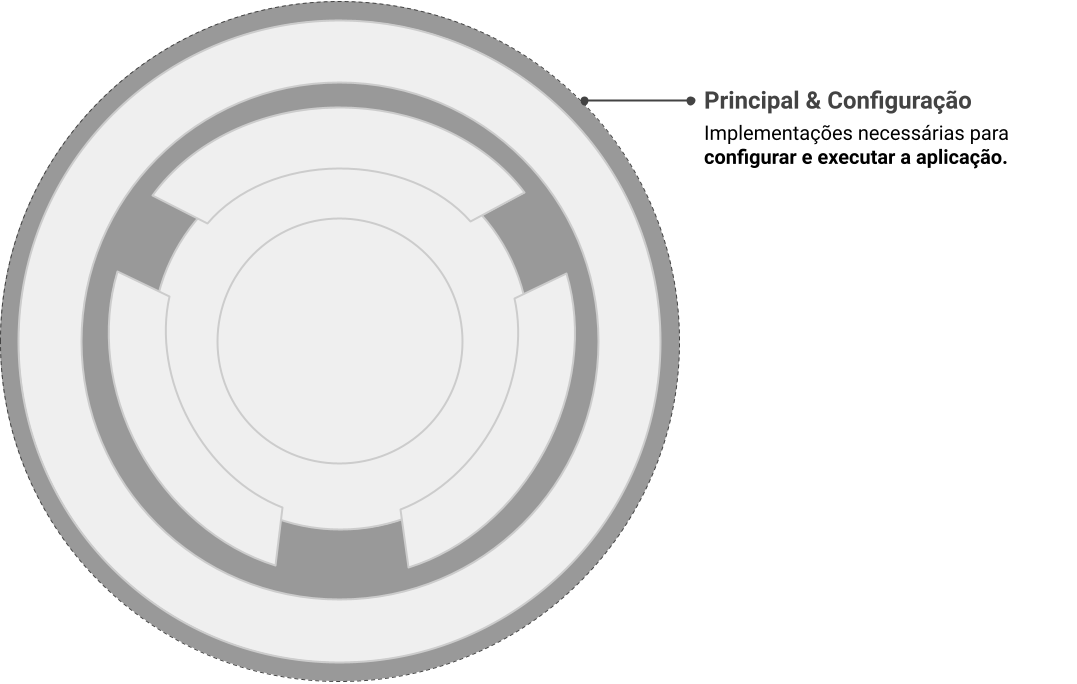
\includegraphics[width=1\textwidth]{images/chapter3-speech2learning-layer5.png}
\fadaptada{FalvoJr2023_HICSS, Lemos2022}
\end{figure}

A Pseudo-camada Principal \& Configuração na arquitetura \textit{Speech2Learning} é assim denominada porque, embora não seja uma camada formal na \textit{Clean Architecture}, desempenha um papel crucial na configuração e inicialização do sistema. Em linhas gerais, esta camada estabelece todas as conexões entre interfaces e suas implementações concretas, além de ser responsável por configurar e executar a aplicação (\autoref{fig:chapter3-speech2learning-layer5}). Além disso, a camada centraliza a configuração e a inicialização, assegurando que todos os componentes estejam devidamente conectados e preparados para operar. As principais responsabilidades desta pseudo-camada incluem:

\begin{itemize}
    \item \textbf{Dependências}: Definir e gerenciar as dependências entre os diferentes componentes do sistema, garantindo que cada componente receba suas dependências de maneira clara e organizada. Isso promove a modularidade e facilita a manutenção do sistema.

    \item \textbf{Inicialização da Aplicação}: Coordenar o processo de inicialização da aplicação, assegurando que todos os componentes sejam configurados e instanciados na ordem correta. Isso inclui a configuração de serviços, repositórios, adaptadores e outros componentes essenciais.

    \item \textbf{Gerenciamento de Ciclo de Vida}: Controlar o ciclo de vida dos componentes, incluindo a criação, a configuração e a destruição de instâncias conforme necessário. Isso assegura que os recursos sejam gerenciados de maneira eficiente e que os componentes estejam sempre em um estado consistente.
\end{itemize}

Alguns exemplos de abstrações alinhadas à \textit{Speech2Learning} para a implementação da Pseudo-camada Principal \& Configuração, são:

\begin{itemize}
    \item \textbf{Módulos de Configuração}: Componentes que centralizam a configuração dos diferentes aspectos da aplicação, como casos de uso, repositórios de dados e serviços de integração. Estes módulos garantem que a configuração seja organizada e fácil de gerenciar.

    \item \textbf{Fábricas de Instâncias}: Abstrações que fornecem métodos para criar e configurar instâncias dos componentes do sistema. As fábricas asseguram que a criação de componentes siga um padrão consistente e que todas as dependências sejam satisfeitas.

    \item \textbf{Controladores de Inicialização}: Componentes responsáveis por coordenar o processo de inicialização da aplicação, garantindo que todos os componentes sejam configurados e preparados para operar. Os controladores de inicialização gerenciam a ordem de inicialização e tratam quaisquer dependências entre os componentes.
\end{itemize}

Para ilustrar a aplicação das abstrações listadas, considere um módulo de configuração que define e gerencia os casos de uso relacionados à transcrição de áudio. Este módulo centraliza a configuração das dependências necessárias para os casos de uso, promovendo a independência e a modularidade dos componentes em relação ao \textit{Spring Framework}. Exemplo em um projeto real disponível no repositório \textit{open-source}: \url{https://bit.ly/S2L-Adapters}.

Estas abstrações e exemplos demonstram como a Pseudo-camada Principal \& Configuração pode ser estruturada. Ao centralizar a configuração e a gestão de dependências, esta camada promove a modularidade e a flexibilidade necessárias para uma solução educacional baseada em reconhecimento de fala.

\section{Considerações Finais}

A arquitetura \textit{Speech2Learning} foi concebida para promover a inclusão e a acessibilidade no domínio educacional, utilizando tecnologias avançadas de reconhecimento de fala, como o ASR e STT. Ao longo deste capítulo foram discutidas a estrutura e as camadas fundamentais da \textit{Speech2Learning}, enfatizando sua modularidade, escalabilidade e conformidade com padrões de mercado. Essas características permitem que a arquitetura seja adaptável a diversos contextos educacionais e atenda às necessidades específicas de diferentes aprendizes, promovendo um ambiente de aprendizagem mais inclusivo e acessível.

A implementação das camadas da \textit{Speech2Learning} demonstrou como a integração de serviços de ASR e STT pode ser realizada de maneira estruturada e eficaz. A arquitetura não só facilita o desenvolvimento de soluções educacionais inclusivas, mas também promove a interoperabilidade entre diferentes plataformas e ferramentas educacionais. Além disso, a adoção de padrões de metadados como Dublin Core, SCORM, MISB, LOM e RDF garante que os OAs sejam estruturados de forma consistente e reutilizável, facilitando o compartilhamento de recursos educacionais.

A sinergia do conceito de IAGen na arquitetura \textit{Speech2Learning} representa um avanço significativo na busca por soluções educacionais mais inclusivas, personalizadas e eficazes. Ao combinar o poder do ASR/STT com a capacidade de processamento de linguagem natural dos LLMs, a \textit{Speech2Learning} torna-se uma ferramenta poderosa para a criação e o acesso a OAs de alta qualidade, que atendem às necessidades de uma ampla gama de aprendizes.

É importante ressaltar que a adoção de IAGen na \textit{Speech2Learning} não é obrigatória, mas sim uma possibilidade que pode ser explorada para aprimorar ainda mais a arquitetura e suas funcionalidades. A flexibilidade da arquitetura permite que diferentes tecnologias e abordagens sejam integradas de acordo com as necessidades e os recursos disponíveis, garantindo que a \textit{Speech2Learning} continue a evoluir e a se adaptar às demandas do cenário educacional em constante transformação.

No próximo capítulo são apresentados os estudos de caso que ilustram a aplicação prática da \textit{Speech2Learning}. O primeiro estudo de caso avalia uma API para a transcrição e legendagem automática de videoaulas, integrando serviços de ASR de fornecedores líderes do mercado. O segundo estudo de caso explora o desenvolvimento de um player de vídeo com integração de avatares de Libras, destacando a importância do design universal para a inclusão de aprendizes surdos. Essas instâncias práticas da \textit{Speech2Learning} não só demonstram a versatilidade e a eficácia da arquitetura, mas também fornecem percepções valiosas sobre a implementação e a avaliação de soluções educacionais baseadas em reconhecimento de fala.

\chapter{Arquitetura Speech2Learning na Prática: Estudos de Caso na Industria}
\label{chapter4}
\section{Considerações Iniciais}

Vimos que a acessibilidade em ambientes de aprendizagem é uma necessidade crescente na era digital, onde as TICs podem desempenhar um papel crucial ao tornar o conteúdos educacionais acessíveis a todos os alunos, independentemente de individualidades físicas ou sensoriais \cite{Mayer2021}. Nesse contexto, investigamos como o enriquecimento de OAs com transcrições/legendas automáticas podem aumentar a inclusão e o engajamento na educação \cite{FalvoJr2023_HICSS,FalvoJr2024_FIE}.

O conceito de OAs é central para as práticas pedagógicas atuais, uma vez que desempenham o papel de recursos digitais flexíveis que podem ser reutilizados para apoiar o processo de ensino-aprendizagem \cite{Parakh2022}. Com isso, a Arquitetura \textit{Speech2Learning} é nossa principal contribuição, através da qual propomos o aprimoramento de OAs audíveis por meio de ASR/STT, promovendo a geração automática de legendas, transcrições ou traduções. Assim, videoaulas podem ser acessíveis em diferentes línguas e até mesmo sinalizadas por avatares de línguas de sinais baseados em texto.

Este capítulo detalha a aplicação prática da \textit{Speech2Learning} por meio de dois Estudos de Caso, projetados como instâncias concretas da arquitetura. Esses estudos foram conduzidos em colaboração com a \textit{EdTech} brasileira DIO, que foi essencial para viabilizar avaliações empíricas em OAs de uma plataforma educacional real, marcando um passo significativo na direção de soluções mais acessíveis e inclusivas.

\section{Estudo de Caso 1: Legendas em Videoaulas}

Nosso primeiro Estudo de Caso buscou investigar a precisão dos principais serviços de ASR, uma vez que essa tecnologia é central na Arquitetura \textit{Speech2Learning}. Na prática, utilizamos um conjunto de recursos educacionais, disponíveis na plataforma de \textit{e-learning} da DIO, para a construção de uma \sigla{PoC}{Prova de Conceito} focada na transcrição e legendagem desses OAs através de serviços de ASR.

Sendo assim, o objetivo deste estudo é expandir nossa compreensão sobre o papel das transcrições e legendas automáticas para um processo de ensino-aprendizagem mais acessível. Para tal propósito, discutimos a convergência dos resultados quantitativos e qualitativos obtidos por meio das três fontes de dados distintas, uma estratégia oriunda da metodologia de triangulação de dados \cite{LimaJunior2021}.

Segundo \cite{Farquhar2020}, é possível explorar múltiplas fontes de evidências (quantitativas e/ou qualitativas) e discutir suas respectivas convergências por meio de uma abordagem de triangulação de dados. No contexto deste Estudo de Caso, as seguintes fontes foram observadas: (i) métodos de similaridade léxica; (ii) respostas de um \textit{Survey} anônimo; e (iii) estudos de uma pesquisa documental complementar.

Desta forma, as seções a seguir abordam desde a implementação da PoC junto a \textit{EdTech} DIO até os detalhes metodológicos e resultados obtidos. Com isso, desenvolvemos discussões e percepções muito interessantes sobre a importância e potencial de TICs como o ASR/STT na promoção de soluções educacionais mais acessíveis.

\subsection{Prova de Conceito: API REST para Legendar Videoaulas}

O desenvolvimento de uma PoC, primeira instância da \textit{Speech2Learning}, surgiu de uma necessidade de negócio da \textit{EdTech} DIO de legendar suas videoaulas de forma escalável. Para isso, uma API REST foi implementada para transcrever videoaulas curtas (entre 15 e 30 segundos), algo comum considerando o conceito de \textit{microlearning} adaptado pela DIO para suas necessidades educacionais. 

Com isso, foi possível explorar os padrões de metadados inerentes à Arquitetura \textit{Speech2Learning} e gerar transcrições e legendas para videoaulas em múltiplos idiomas. Nesse sentido, definimos o escopo da PoC aos idiomas suportados na plataforma da DIO: Português, Inglês e Espanhol. Desta forma, foi possível ampliar a acessibilidade desses OAs por meio de transcrições e legendas geradas automaticamente a priori.

Conforme o diagrama da \autoref{fig:chapter4-cs1-poc-diagram}, a API REST segue as diretrizes da \textit{Speech2Learning}, bem como apresenta uma visão da estrutura de C\&C \cite{Bass2021}. O esquema de cores dos componentes corresponde ao das camadas na \autoref{fig:chapter3-speech2learning-arch}, ilustrando uma implementação em conformidade com os limites lógicos/estruturais pré-definidos para uma API REST.

\begin{figure}[htb]
\centering
\caption{Visão 1ª Instância da \textit{Speech2Learning}: API REST para Legendar Videoaulas}
\label{fig:chapter4-cs1-poc-diagram}
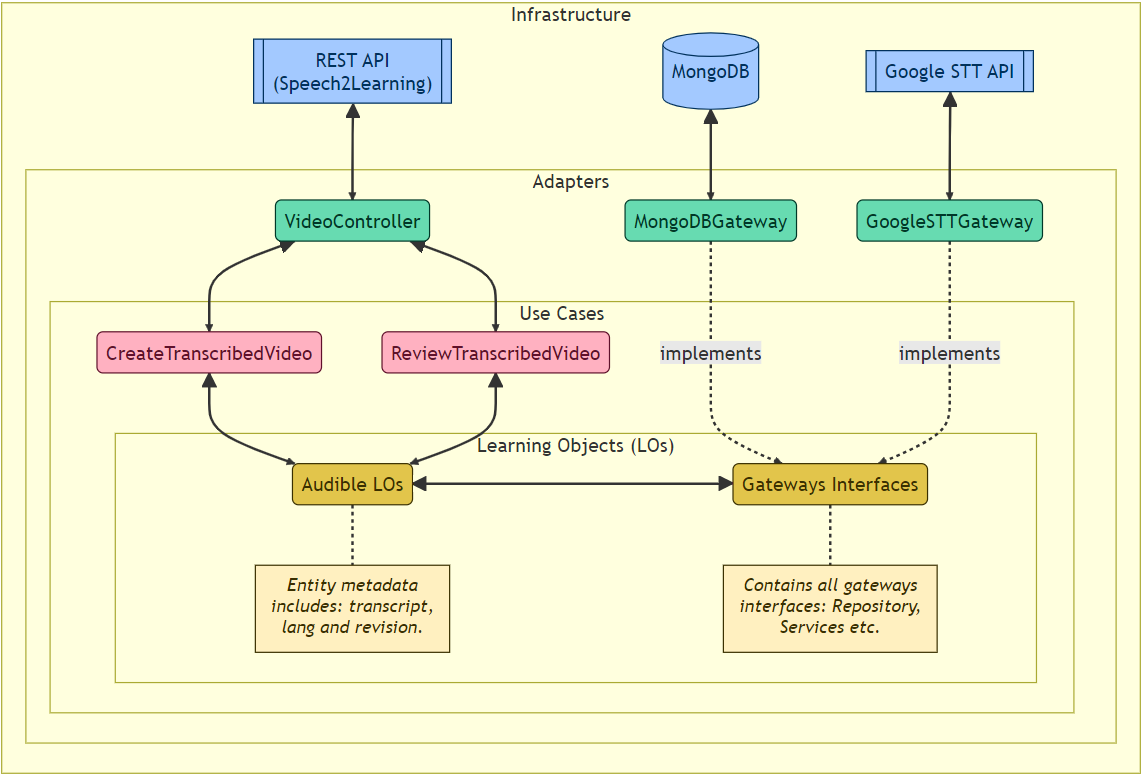
\includegraphics[width=\columnwidth]{images/chapter4-cs1-poc-diagram.png}
\fdireta{FalvoJr2023_HICSS}
\end{figure}

O diagrama define dois \textit{Casos de Uso} relacionados à transcrição de vídeos: \textit{Criar} e \textit{Revisar}. Esta visão é interessante pois esclarece as funcionalidades implementadas na PoC. Além disso, nossas entidades foram projetadas como \textit{OAs Audíveis}, uma vez que lidamos com videoaulas. Para concluir, detalhes sobre a implementação também são expostos claramente na camada de \textit{Infraestrutura}. Por exemplo, nosso ponto de entrada é uma \textit{API REST}, o \textit{MongoDB} é o banco de dados e \textit{Google STT API} (API externa) é o provedor de STT.

Para oferecer uma perspectiva mais técnica, a PoC pode ser consumida sob demanda através de uma requisição HTTP POST para uma API REST reativa. Este endpoint aciona um fluxo de trabalho assíncrono para extrair o áudio do vídeo, otimizando assim o consumo de largura de banda antes de invocar a \textit{Google STT API}. Após a resposta dessa requisição, a transcrição é armazenada nos metadados do \textit{OA Audível}, tornando essa transcrição automática elegível para revisão.

Para revisar a transcrição de um OA existente, basta fazer uma requisição HTTP PUT para atualizar este recurso, versionando suas transcrições por meio dos metadados. Vale lembrar que, a \textit{Speech2Learning} apenas define diretrizes para a criação de soluções baseadas em STT para promover a acessibilidade de OAs, sem impor decisões de design, tecnologias ou aspectos de segurança.

Na prática, o acesso à PoC foi restrito à Equipe de Educação da DIO, garantindo que seus OAs (videoaulas) fossem criados e revisados com segurança e em um ambiente controlado. Ressaltamos que as transcrições automáticas exigiram uma extensa revisão por especialistas em línguas da empresa, destacando a necessidade de otimizar o processo de transcrição e explorar outros serviços de STT.

Inspirados pelos \textit{insights} e desafios desta PoC, pensamos em expandir nossas percepções por meio de um Estudo de Caso mais amplo. Por sua vez, esta iniciativa de investigação visa analisar mais profundamente as nuances entre diferentes provedores de STT. Portanto, para nosso Estudo de Caso, selecionamos 15 videoaulas cujas transcrições foram revisadas por especialistas em idiomas da DIO durante a PoC. Esta quantidade e duração de vídeos foram estrategicamente definidas para controle financeiro (custo dos provedores de STT) e, principalmente, viabilizar um \textit{Survey} coeso para avaliação da precisão das transcrições automáticas sob novas perspectivas.

Para uma análise mais robusta, procuramos diversificar as línguas e os professores das videoaulas, de forma a captar diferentes sotaques e regionalidades. A \autoref{tab:chapter4-poc-audios-summary} detalha as características linguísticas e técnicas dos áudios extraídos das videoaulas. Este conjunto diversificado de dados servirá como referência, nos permitindo analisar criticamente o desempenho de outros fornecedores de STT em múltiplos contextos de ensino-aprendizagem.

\begin{table}[htb]
\centering
\caption{\textit{Dataset} do Estudo de Caso 1 (Áudios Extraídos das Videoaulas)}
\label{tab:chapter4-poc-audios-summary}
\begin{tabular}{|c|c|c|c|l|c|}
\hline
\textbf{ID} & \textbf{Língua} & \textbf{Sotaque} & \textbf{Gênero} & \textbf{Tópico Educacional} & \textbf{Tempo} \\ \hline
1 & pt-BR & BRA & M & Apps Android & 0:17 \\ \hline
2 & pt-BR & BRA & M & SCRUM & 0:26 \\ \hline
3 & pt-BR & BRA & F & Selenium WebDriver & 0:23 \\ \hline
4 & pt-BR & BRA & F & Blockchain & 0:20 \\ \hline
5 & pt-BR & BRA & M & Kernel Híbrido & 0:24 \\ \hline
6 & en-US & BRA & F & Visto de Trânsito & 0:29 \\ \hline
7 & en-US & USA & Ambos & Entrevista de Emprego & 0:16 \\  \hline
8 & en-US & BRA & F & Oportunidades de Emprego & 0:20 \\  \hline
9 & en-US & BRA & F & Liderança Servidora & 0:15 \\  \hline
10 & en-US & BRA & M & Goroutines & 0:15 \\  \hline
11 & es-AR & ARG & F & Lógica de Programação & 0:12 \\  \hline
12 & es-AR & ARG & F & Linguagens de programação & 0:21 \\  \hline
13 & es-AR & ARG & F & Tipos de Dados em Python & 0:14 \\  \hline
14 & es-AR & ARG & F & Hello World com Python & 0:17 \\  \hline
15 & es-AR & ARG & F & String Slicing com Python & 0:26 \\ \hline
\end{tabular}
\fadaptada{FalvoJr2023_HICSS}
\end{table}

Este conjunto de dados (\textit{dataset}) passou por um rigoroso controle de qualidade de áudio, protocolo padrão para todo conteúdo oferecido na plataforma educacional da DIO. Para garantir a transparência dessas informações, disponibilizamos uma pasta pública\footnote{\textit{Dataset} do Estudo de Caso 1: \url{https://bit.ly/S2L-Audios}} que contém todas as amostras de áudio suas respectivas transcrições revisadas por especialistas em línguas da DIO. 

Tecnicamente, o \textit{dataset} atende ou excede os seguintes critérios de qualidade: canais de áudio duplos, taxa de amostragem de 44,1 kHz e precisão de 16 bits. Tais aspectos técnicos não só garantem excelente qualidade de som, mas também contribuem para transcrições automáticas mais precisas.

Nesse contexto, a realização de um Estudo de Caso é uma excelente opção para ampliar esta PoC e orientar análises e discussões mais profundas. Resumidamente, a PoC identificou a necessidade de reduzir o retrabalho exigido na revisão das transcrições automáticas e assim melhorar a eficiência do processo de transcrição. Esta progressão da PoC para um Estudo de Caso reflete uma abordagem comum em pesquisa que permite o desenvolvimento iterativo \cite{Runeson2009}. 

O \textit{dataset} compilado nesta PoC nos permitiu analisar a qualidade das transcrições automáticas em vários provedores de STT, usando as transcrições de referência revisadas pelos especialistas em idiomas da DIO como um controle confiável. A metodologia definida para o Estudo de Caso decorrente desta PoC, bem como seus resultados são apresentados a seguir.

\subsection{Metodologia}

Esta seção descreve a metodologia deste Estudo de Caso, com o objetivo de investigar o papel do ASR e do STT na melhoria da acessibilidade de OAs. Trata-se de uma investigação empírica, apoiada em raciocínio indutivo e pesquisa de campo. Ao contrário dos estudos experimentais, os Estudos de Caso reúnem informações de diversas fontes por meio de diferentes técnicas de coleta de dados \cite{Sommerville2015}.

Como dito anteriormente, firmamos uma parceria com a \textit{EdTech} DIO, que compartilhou conosco videoaulas disponíveis em seu currículo, oferecendo uma oportunidade de conexão entre a indústria e nossa pesquisa. A DIO concedeu acesso a parte de sua infraestrutura em nuvem, além de disponibilizar especialistas em línguas que revisaram os resultados do ASR durante a PoC. Esse processo de revisão foi fundamental para que as fontes de evidência, baseadas na precisão das transcrições e legendas de videoaulas, tivessem referências sólidas para nossas comparações e análises.

Como consequência, tanto os dados de similaridade léxica quanto as respostas do \textit{Survey} avaliaram o mesmo conjunto de 15 videoaulas: 5 em inglês, 5 em português e 5 em espanhol. Essa abordagem facilitou a obtenção de duas perspectivas quantitativas distintas sobre a qualidade das transcrições automáticas: uma derivada de algoritmos de similaridade léxica e a outra baseada nas percepções dos aprendizes.

Adicionalmente, nossa metodologia integra um terceiro aspecto de coleta de dados através de uma pesquisa documental focada em ASR/STT, além de aplicar a Teoria Fundamentada \cite{Charmaz2009} para assegurar um processo de análise de conteúdo. Portanto, nossa pesquisa documental visa fornecer dados qualitativos sobre o fenômeno observado \cite{LimaJunior2021}.

Ao triangular os dados coletados de similaridade léxica, das respostas do \textit{Survey} anônimo e da pesquisa documental complementar (\autoref{fig:chap4:triangulation-sources}), buscamos oferecer uma compreensão abrangente dos desafios e oportunidades associados à utilização de tecnologias ASR para aumentar a acessibilidade de OAs no domínio educacional. 

\begin{figure}[htb]
\centering
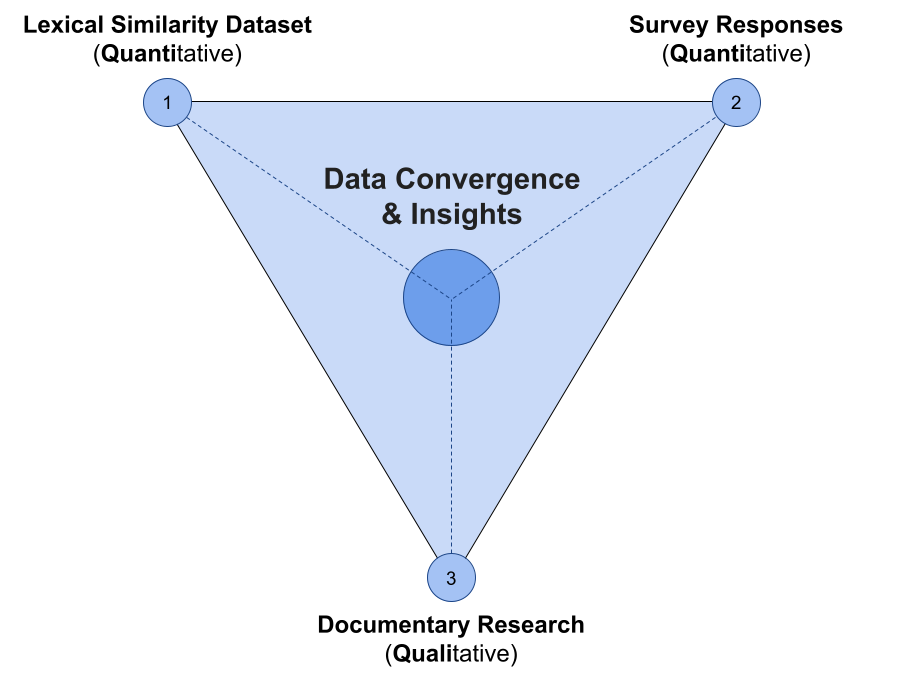
\includegraphics[width=0.75\textwidth]{images/chapter4-cs1-triangulation-sources.png}
\caption{Triangulação de Dados: Fontes de Evidência.}
\label{fig:chap4:triangulation-sources}
\fdireta{FalvoJr2024_FIE}
\end{figure}

A seguir, delineamos cada fonte de evidência e suas técnicas de coleta, esclarecendo todo o processo de triangulação e sua contribuição para uma compreensão robusta do impacto das tecnologias ASR, como o STT, na acessibilidade educacional.

\subsubsection{1ª Fonte de Evidência: Métodos de Similaridade Léxica}

Esta seção apresenta a metodologia definida para a primeira fonte de evidências da triangulação de dados, onde métodos de similaridade léxica têm como objetivo avaliar e identificar o provedor de ASR/STT mais assertivo para transcrição automática. Nesse sentido, algoritmos de similaridade léxica são métricas particularmente relevantes para a avaliação da precisão de transcrições automáticas, conforme discutimos detalhadamente em \citeonline{FalvoJr2023_HICSS}.

Medir a semelhança entre textos é uma prática comumente investigada em pesquisas acadêmicas, em geral apoiada por métodos de análise/similaridade léxica \cite{Majumdar2022}. Para comparar nossas transcrições automáticas e de referência, precisamos definir como extrairemos nossos dados quantitativos utilizando técnicas de similaridade léxica. No nosso contexto, algumas das alternativas mais interessantes são:

\begin{itemize}

\item \textbf{\sigla{CS}{Similaridade de Cosseno}}: Esta métrica é usada para medir a similaridade entre dois vetores. Especificamente, ela mede a semelhança na direção ou orientação dos vetores, ignorando as diferenças na sua magnitude ou escala. Ambos os vetores devem pertencer ao mesmo espaço de produto interno, o que significa que devem produzir um escalar ao multiplicar o produto interno. A similaridade de dois vetores é medida pelo cosseno do ângulo entre eles. A métrica CS varia de 0 a 1, onde um valor mais próximo de 0 indica menor similaridade e um valor mais próximo de 1 indica maior similaridade \cite{cosseno-1,cosseno-2,cosseno-3}.

\item \textbf{\sigla{JI}{Índice de Jaccard}}: Esta métrica é definida como a interseção de dois conjuntos de dados dividida pela união desses conjuntos, medindo a similaridade entre eles. No contexto de textos, pode ser expressa como o número de palavras comuns dividido pelo número total de palavras nos dois textos ou documentos. O JI varia de 0 a 1, onde 0 significa nenhuma similaridade e 1 significa sobreposição completa. O JI é calculado dividindo o número de observações em ambos os conjuntos pelo número de observações em cada conjunto, ou seja, o tamanho da interseção dividido pelo tamanho da união de dois conjuntos \cite{Majumdar2022,jaccard-1,jaccard-2}.

\item \textbf{\sigla{LD}{Distância de Levenshtein}}: Esta métrica de \textit{string} mede a diferença entre duas strings. Basicamente, a LD entre duas palavras é o número mínimo de edições de um único caractere (inserções, exclusões ou substituições) necessárias para transformar uma palavra na outra. Seu nome é uma homenagem a Vladimir Levenshtein, que considerou essa distância em 1965. A comparação LD é geralmente realizada entre duas palavras, determinando o número mínimo de edições necessárias para alterar uma palavra para outra. Quanto maior o número de edições, maior a diferença entre os textos. Uma edição é definida como a inserção, exclusão ou substituição de um caractere \cite{levens-1,levens-2}.

\end{itemize}

Neste estudo, aplicamos os três métodos mencionados, destacando sua relevância em nossa metodologia. Primeiramente, geramos e revisamos as transcrições de referência usando a instância da \textit{Speech2Learning}, desenvolvida como uma PoC. Em seguida, transcrevemos automaticamente cada OA utilizando diferentes serviços de ASR/STT, permitindo a comparação entre as transcrições de referência e as automáticas. Dessa forma, utilizamos os métodos de similaridade léxica CS, JI e LD como métricas de precisão.

Para essa finalidade, identificamos os principais provedores de ASR/STT baseados em IA do mercado \cite{Gartner2023}: Amazon, Google, IBM, Microsoft e OpenAI. Ademais, em colaboração com a DIO, garantimos que todos os OAs e suas transcrições de referência estavam devidamente revisadas e disponíveis no \textit{dataset} deste Estudo de Caso (\autoref{tab:chapter4-poc-audios-summary}).

Com os áudios otimizados do \textit{dataset}, integramos os serviços de ASR/STT de cada provedor e geramos suas respectivas transcrições automáticas. Para uma implementação organizada e documentada, utilizamos o Google Colab, detalhando todo o processo em um notebook público\footnote{Colab Notebook - Transcrições Automáticas com ASR/STT: \url{https://bit.ly/S2L-STTServices}}. De forma similar, comparamos as 15 transcrições automáticas com as transcrições de referência usando os três métodos de similaridade léxica (CS, JI e LD) em um segundo notebook\footnote{Colab Notebook - Algoritmos de Similaridade Léxica: \url{https://bit.ly/S2L-CaseStudy}}.

\subsubsection{2ª Fonte de Evidência: Respostas do \textit{Survey}}

Conduzimos um \textit{Survey} para avaliar as percepções dos alunos sobre a qualidade das transcrições automáticas fornecidas por ASR/STT. Este \textit{Survey} coletou feedbacks quantitativos e qualitativos de participantes com experiência em Tecnologia da Informação (TI) ou Linguística e Educação. Disponibilizamos uma cópia em \url{https://bit.ly/S2L-Survey} para que a dinâmica do formulário seja compreendida completamente.

O \textit{Survey} utilizou uma combinação de perguntas de escala Likert e perguntas abertas. As perguntas de escala Likert visavam avaliar quantitativamente a coerência/qualidade das transcrições em três idiomas (inglês, português e espanhol). Esta consistência no conteúdo permitiu uma comparação direta das avaliações técnicas e centradas no usuário. As perguntas abertas buscavam obter \textit{insights} qualitativos sobre a eficácia percebida das soluções de ASR. No entanto, devido à conformidade ética, não exploraremos os dados qualitativos neste estudo.

Os participantes avaliaram as transcrições do mesmo conjunto de 15 videoaulas (cinco por idioma) e dos mesmos cinco provedores (Amazon, Google, IBM, Microsoft e OpenAI) utilizados no estudo de similaridade léxica. Este alinhamento entre as duas fontes garantiu que as Respostas do Survey complementassem diretamente a análise técnica de similaridade léxica, proporcionando uma visão holística do desempenho das transcrições.

Para mitigar vieses, os provedores foram anonimizados e receberam um identificador numérico aleatório em vez de serem nomeados, garantindo que as avaliações refletissem experiências genuínas dos usuários, sem influência do reconhecimento da empresa/marca. Esta abordagem metodológica está alinhada às melhores práticas em metodologia de pesquisa empírica, conforme defendido por \cite{Sommerville2015}, especialmente na coleta de feedback e percepções dos usuários em estudos de engenharia de software.

\subsubsection{3ª Fonte de Evidência: Pesquisa Documental}

Para contextualizar e enriquecer nossos dados quantitativos, realizamos uma revisão de literatura que complementa nossos achados empíricos, identificando estudos relevantes sobre tecnologias ASR e STT. Esta revisão proporciona uma compreensão mais profunda do potencial e das limitações das tecnologias atuais baseadas em ASR.

Empregamos a \textit{Grounded Theory}, ou \sigla{TFD}{Teoria Fundamentada nos Dados}, como um \textit{framework} orientador para nossa análise documental. A TFD é uma metodologia sistemática e rigorosa utilizada na pesquisa qualitativa para desenvolver teorias emergentes diretamente dos dados \cite{Charmaz2009}. Diferentemente de abordagens que partem de hipóteses preconcebidas, a Teoria Fundamentada nos Dados permite a descoberta de temas e padrões de maneira indutiva, por meio de um processo iterativo de coleta e análise de dados.

Neste estudo, utilizamos a TFD para examinar os estudos selecionados na pesquisa documental. Este processo incluiu a codificação aberta dos dados, a identificação de temas recorrentes e a integração desses temas em uma teoria coesa. Assim, garantimos que nossas conclusões fossem baseadas diretamente nas evidências coletadas, sem impor noções preconcebidas.

Nossa pesquisa documental envolveu uma revisão complementar da literatura, incluindo artigos, livros e relatórios, focando nas tecnologias ASR e STT no contexto da acessibilidade educacional. Através dessa análise, buscamos identificar temas recorrentes, diretrizes teóricas e lacunas nas pesquisas existentes, contribuindo para uma compreensão mais detalhada do assunto.

Ao integrar \textit{insights} do Conjunto de Dados de Similaridade Lexical, das Respostas do \textit{Survey} e da Pesquisa Documental, visamos fornecer uma exploração abrangente e multidimensional do papel do ASR e do STT na melhoria da acessibilidade educacional.

\subsubsection{Nossa Triangulação de Dados}

A triangulação, originalmente uma técnica geométrica para determinação de localização, evoluiu para uma metáfora representando métodos de pesquisa que integram diversas abordagens, teorias ou fontes de dados. Essa integração permite uma compreensão mais abrangente de um fenômeno, sendo especialmente útil na pesquisa qualitativa. A triangulação aumenta a validade de um estudo ao empregar vários métodos para verificar ou corroborar um evento, descrição ou fato específico, reforçando assim a credibilidade e a confiabilidade do estudo \cite{Farquhar2020, Yin2015}.

Neste estudo, adotamos uma abordagem de triangulação que engloba múltiplas fontes de evidência e suas respectivas técnicas. Esta abordagem de métodos mistos combina resultados qualitativos e quantitativos para aprimorar a análise e a interpretação dos dados coletados. Em particular, aplicamos a triangulação de dados, que utiliza várias fontes de evidência para corroborar o mesmo fato ou fenômeno \cite{Yin2015}.

Na ES, a triangulação contribui significativamente para o rigor e a validade da pesquisa. A integração de vários métodos, como pesquisas quantitativas, entrevistas qualitativas e análise documental, permite aos pesquisadores verificar os resultados de forma cruzada e obter uma compreensão mais aprofundada de fenômenos complexos. Esta abordagem é particularmente valiosa na análise da eficácia das práticas de desenvolvimento de software, experiência do usuário e adoção de tecnologias \cite{Runeson2009}.

A \autoref{fig:chapter4-cs1-triangulation-methodology} representa nossa metodologia de triangulação de dados. Este diagrama esboça o objeto de estudo, as três fontes distintas de evidência, suas respectivas técnicas de coleta e o processo de convergência de dados que resulta em nosso corpus de dados. Esta abordagem completa e multifacetada garante uma validação robusta e proporciona uma compreensão profunda de como as tecnologias ASR podem melhorar a acessibilidade educacional.

\begin{figure}[htb]
\centering
\caption{Nossa Metodologia de Triangulação de Dados.}
\label{fig:chapter4-cs1-triangulation-methodology}
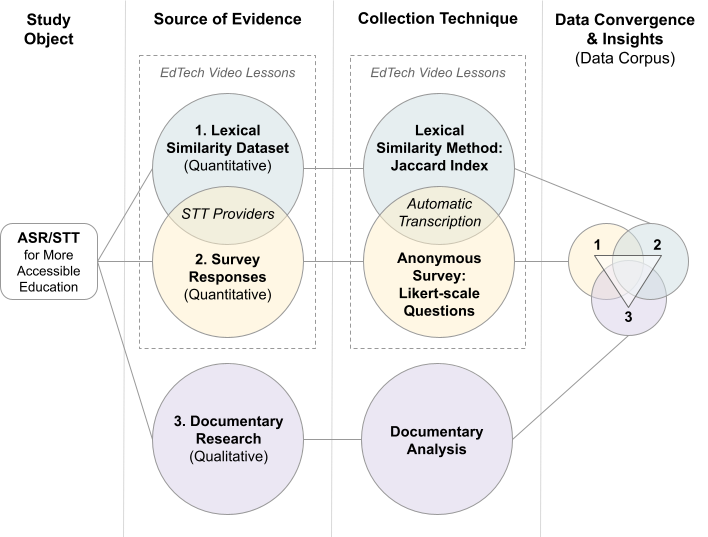
\includegraphics[width=0.9\textwidth]{images/chapter4-cs1-triangulation-methodology.png}
\fdireta{FalvoJr2024_FIE}
\end{figure}

Para as fontes de evidência quantitativas, similaridade léxica e respostas do \textit{Survey}, estabelecemos dois conjuntos de hipóteses que guiarão nossa análise. No nosso contexto, hipóteses compartilhadas fazem sentido porque ambas as fontes de evidência exploram as mesmas videoaulas e avaliam os mesmos provedores. Sendo assim, primeiro consideramos a comparação entre diferentes provedores de transcrição automática, independentemente do idioma. As hipóteses são formuladas da seguinte maneira:

\begin{itemize}
\item \textbf{Hipótese Nula ($H^0$)}: Não há diferença estatisticamente significativa na qualidade das transcrições automáticas entre os provedores.
\item \textbf{Hipótese Alternativa ($H^1$)}: Há uma diferença estatisticamente significativa na qualidade das transcrições automáticas entre os provedores.
\end{itemize}

Em segundo lugar, avaliamos a qualidade das transcrições automáticas considerando os idiomas Português, Inglês e Espanhol. As hipóteses são delineadas conforme segue:

\begin{itemize}
\item \textbf{Hipótese Nula ($H^0$)}: Não há diferença estatisticamente significativa na qualidade das transcrições automáticas para Português, Inglês e Espanhol entre os provedores.
\item \textbf{Hipótese Alternativa ($H^1$)}: Há uma diferença estatisticamente significativa na qualidade das transcrições automáticas para Português entre os provedores.
\item \textbf{Hipótese Alternativa ($H^2$)}: Há uma diferença estatisticamente significativa na qualidade das transcrições automáticas para Inglês entre os provedores.
\item \textbf{Hipótese Alternativa ($H^3$)}: Há uma diferença estatisticamente significativa na qualidade das transcrições automáticas para Espanhol entre os provedores.
\end{itemize}

Para a pesquisa documental, adotamos uma abordagem qualitativa para investigar de maneira mais ampla e exploratória como as tecnologias de reconhecimento de fala para transcrição automática (ASR e STT) influenciam a acessibilidade dos OAs. A questão de pesquisa que orienta nossa análise documental é:

\begin{itemize}
\item \textbf{Questão de Pesquisa}: Como as tecnologias de reconhecimento de fala (ASR/STT) podem contribuir para uma educação mais acessível?
\end{itemize}

Essa combinação de hipóteses quantitativas e uma questão de pesquisa qualitativa permite uma triangulação robusta de dados, fornecendo uma visão abrangente e multidimensional do impacto das tecnologias de ASR/STT na acessibilidade educacional. A análise das respostas do \textit{Survey}, juntamente com os métodos de similaridade léxica e a pesquisa documental, nos permitirá identificar as convergências entre nossas fontes de evidências e enriquecer as discussões, fortalecendo a validade do estudo.

Para fornecer uma visão formal, mas simplificada, deste primeiro Estudo de Caso, sintetizamos suas principais características na Tabela \autoref{tab:chapter4-cs1-summary}. Esta síntese foi elaborada seguindo as diretrizes metodológicas e as perspectivas de pesquisa descritas por \citeonline{CastroFilho2021}, garantindo uma abordagem estruturada e coerente com os padrões de pesquisa científica em informática na educação.

\begin{table}[htb]
\centering
\caption{Síntese do Estudo de Caso 1: Legendas Automáticas em Videoaulas}
\label{tab:chapter4-cs1-summary}
\begin{tabular}{|C{3cm}|m{11.75cm}|}\hline
\textbf{Objeto de Estudo} & Serviços de Reconhecimento de Fala (ASR/STT) \\\hline
\textbf{Perspectiva} & Explanatória (Explicativa) \\\hline
\textbf{Característica} & Explicação de causas ou efeitos relacionais ao fenômeno \cite{CastroFilho2021}. \\\hline
\textbf{Objetivos} & \begin{tabular}[c]{@{}m{11.75cm}@{}}1. Avaliar a qualidade das transcrições automáticas fornecidas por diferentes serviços de ASR/STT. \\ 2. Investigar a variação na qualidade das transcrições automáticas em diferentes idiomas (Português, Inglês e Espanhol). \\ 3. Explorar como as transcrições automáticas podem melhorar a acessibilidade educacional.\end{tabular} \\\hline
\textbf{Questões de Pesquisa} & Como as tecnologias de reconhecimento de fala (ASR/STT) podem contribuir para uma educação mais acessível? \\\hline
\textbf{Hipóteses} & \begin{tabular}[c]{@{}m{11.75cm}@{}}1. Existe diferença estatisticamente significativa na precisão das transcrições automáticas entre os provedores de ASR/STT. \\ 2. Existe diferença estatisticamente significativa na precisão das transcrições automáticas para Português, Inglês e Espanhol entre os provedores de ASR/STT.\end{tabular} \\\hline
\textbf{Fontes de Dados} & \begin{tabular}[c]{@{}m{11.75cm}@{}}1. Dados quantitativos de métodos de similaridade léxica (precisão). \\ 2. Respostas quantitativas de um \textit{Survey} anônimo (precisão). \\ 3. Dados qualitativos de uma pesquisa documental.\end{tabular} \\\hline
\textbf{Método de Coleta de Dados} & \begin{tabular}[c]{@{}m{11.75cm}@{}}Triangulação de Dados, com as seguintes fontes de evidência: \\ 1. Métodos de Similaridade Léxica. \\ 2. Respostas do \textit{Survey}. \\ 3. Pesquisa Documental.\end{tabular} \\\hline
\textbf{Tipo de Análise} & Mista (Quantitativa e Qualitativa) \\\hline
\end{tabular}
\end{table}

\subsection{Resultados e Discussões}

\subsubsection{Métodos de Similaridade Léxica}

Considerando nossas fontes de evidência quantitativas, usamos um \textit{dataset} projetado para avaliar a qualidade das transcrições automáticas de provedores líderes de ASR/STT (Amazon, Google, IBM, Microsoft e OpenAI) através de três métricas de similaridade léxica (CS, JI e LD). Nesse sentido, considerando as características dos dados coletados, focamos no JI devido ao seu desempenho estatístico mais robusto, sendo nossa única amostra com distribuição normal.

Lembrando que, o método de Jaccard mede a similaridade entre dois conjuntos de dados calculando o tamanho da interseção dividido pelo tamanho da união dos conjuntos de amostras. No nosso contexto, ele compara as palavras da transcrição automática com as da transcrição de referência (revisada por especialistas), proporcionando uma medida quantitativa de precisão. 

Sendo assim, vamos apresentar os resultados do JI como métrica principal de similaridade léxica para avaliar os provedores de ASR/STT. Os achados iniciais desta fonte de evidência podem ser visualizados por meio do conjunto de gráficos da \autoref{fig:chapter4-cs1-lexical-all}.

\begin{figure}[htbp]
\centering
\caption{Índice de Jaccard: Gráficos dos Provedores Sem Agrupar Por Idioma.}
\label{fig:chapter4-cs1-lexical-all}
\begin{subfigure}[b]{0.8\textwidth}
\centering
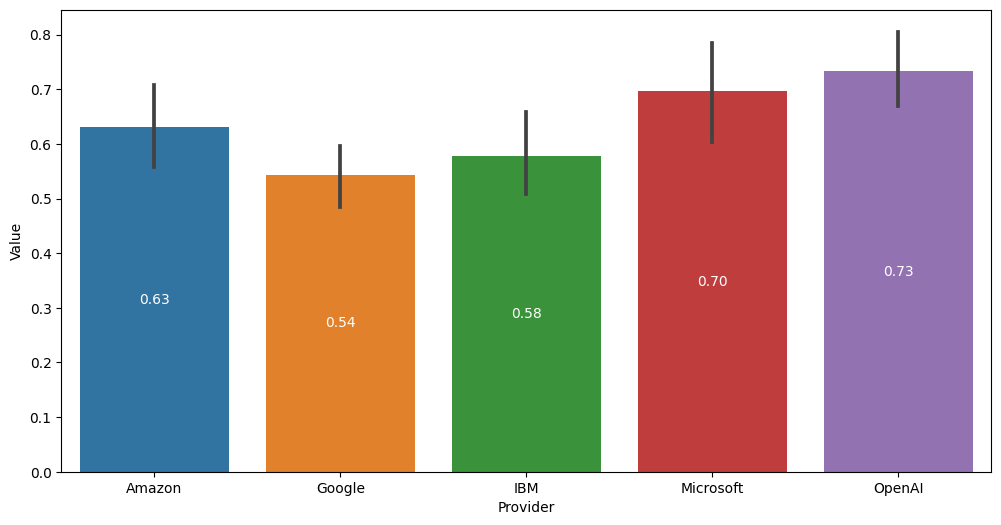
\includegraphics[width=\textwidth]{images/chapter4-cs1-lexical-all-barplot.png}
\caption{Gráfico de Barras.}
\label{fig:chapter4-cs1-lexical-all-barplot}
\end{subfigure} ~
\begin{subfigure}[b]{0.8\textwidth}
\centering
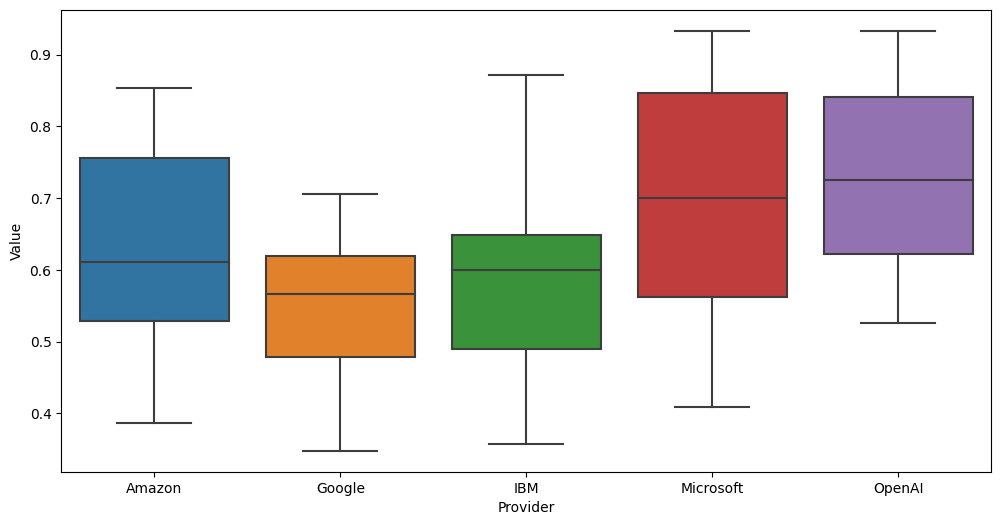
\includegraphics[width=\textwidth]{images/chapter4-cs1-lexical-all-boxplot.png}
\caption{Gráfico de Boxplot.}
\label{fig:chapter4-cs1-lexical-all-boxplot}
\end{subfigure} ~
\begin{subfigure}[b]{0.8\textwidth}
\centering
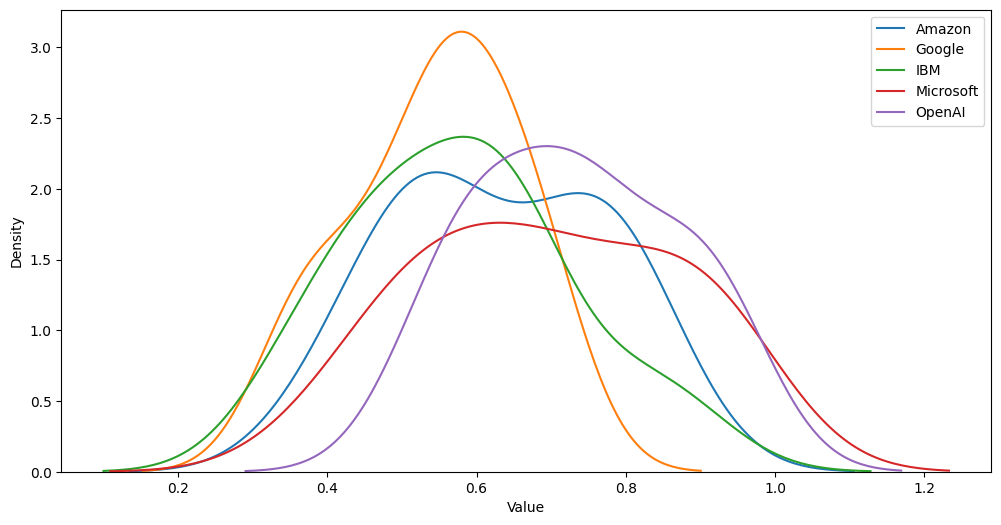
\includegraphics[width=\textwidth]{images/chapter4-cs1-lexical-all-kdeplot.png}
\caption{Gráfico KDE.}
\label{fig:chapter4-cs1-lexical-all-kdeplot}
\end{subfigure}
\fadaptada{FalvoJr2023_HICSS}
\end{figure}

A \autoref{fig:chapter4-cs1-lexical-all} inclui um Gráfico de Barras (\ref{fig:chapter4-cs1-lexical-all-barplot}) que exibe o JI médio para cada provedor, um \textit{Boxplot} (\ref{fig:chapter4-cs1-lexical-all-boxplot}) que detalha a distribuição dos dados e um Gráfico KDE (\ref{fig:chapter4-cs1-lexical-all-kdeplot}) que ilustra a densidade de probabilidade das pontuações. Essas visualizações destacaram proeminentemente a OpenAI, que demonstrou a maior pontuação, sugerindo seu desempenho superior na captura da similaridade léxica em várias aplicações de transcrição.

As análises estatísticas detalhadas na \autoref{tab:chapter4-results-ji-tests} corroboram as impressões iniciais dos gráficos. Os testes de normalidade, o \textit{Kolmogorov-Smirnov} \cite{Kolmogorov1933,Smirnov1948} e o \textit{Shapiro-Wilk} \cite{Shapiro1965}, confirmaram a distribuição normal dos dados, permitindo uma análise adicional por meio da \textit{One-Way ANOVA} \cite{Fisher1925}. 

Por sua vez, o teste de ANOVA revelou diferenças significativas entre os provedores. Portanto, as análises \textit{post-hoc} de \textit{Tukey HSD} \cite{Tukey1949} e de \textit{Bonferroni} \cite{Bonferroni1936} foram aplicadas para identificar essas diferenças explicitamente. 

\begin{table}[htb]
\centering
\caption{Testes Estatísticos do Índice de Jaccard: Provedores Sem Agrupar Por Idioma}
\label{tab:chapter4-results-ji-tests} 
\begin{tabular}{lcclc|}
\hline
\multicolumn{5}{|c|}{\textbf{Tests of Normality}} \\ \hline
\multicolumn{1}{|c|}{\multirow{2}{*}{\textbf{Test}}} & \multicolumn{2}{c|}{\textbf{Kolmogorov-Smirnov}} & \multicolumn{2}{c|}{\textbf{Shapiro-Wilk}} \\ \cline{2-5} 
\multicolumn{1}{|c|}{} & \multicolumn{1}{c|}{\textbf{Statistic}} & \multicolumn{1}{c|}{\textbf{Significance \ensuremath{(p)}}} & \multicolumn{1}{c|}{\textbf{Statistic}} & \textbf{\ensuremath{p}} \\ \hline
\multicolumn{1}{|c|}{Jaccard Index} & \multicolumn{1}{c|}{0.057} & \multicolumn{1}{c|}{\textbf{0.200}} & \multicolumn{1}{c|}{0.973} & \textbf{0.111} \\ \hline
\multicolumn{5}{|c|}{\textbf{Interpretation}} \\ \hline
\multicolumn{5}{|l|}{\begin{tabular}[c]{@{}l@{}}Kolmogorov-Smirnov: If \ensuremath{p>0.05}, sample follow the same statistical distribution.\end{tabular}} \\ \hline
\multicolumn{5}{|l|}{Shapiro-wilk: If \ensuremath{p>0.05} is normal.} \\ \hline
\multicolumn{5}{|c|}{\textbf{One-Way ANOVA (One-Way Analysis of Variance)}} \\ \hline
\multicolumn{1}{|c|}{\textbf{Test}} & \multicolumn{2}{c|}{\textbf{F}} & \multicolumn{2}{c|}{\textbf{\ensuremath{p}}} \\ \hline
\multicolumn{1}{|c|}{Jaccard Index} & \multicolumn{2}{c|}{4.562} & \multicolumn{2}{c|}{\textbf{0.002}} \\ \hline
\multicolumn{5}{|c|}{\textbf{Interpretation}} \\ \hline
\multicolumn{5}{|l|}{\begin{tabular}[c]{@{}l@{}}If \ensuremath{p<0.05}, there are significant differences between at least two groups.\end{tabular}} \\ \hline
\multicolumn{5}{|c|}{\textbf{Tukey HSD (Honest Significant Difference)}} \\ \hline
\multicolumn{3}{|l|}{\textbf{Providers (Groups from 1 to 5)}} & \multicolumn{2}{c|}{\textbf{\ensuremath{p}}} \\ \hline
\multicolumn{3}{|l|}{OpenAI (Group 5) to Google (Group 2)} & \multicolumn{2}{c|}{\textbf{0.005}} \\ \hline
\multicolumn{3}{|l|}{OpenAI (Group 5) to IBM (Group 3)} & \multicolumn{2}{c|}{\textbf{0.032}} \\ \hline
\multicolumn{3}{|l|}{Microsoft (Group 4) to Google (Group 2)} & \multicolumn{2}{c|}{\textbf{0.037}} \\ \hline
\multicolumn{5}{|c|}{\textbf{Interpretation}} \\ \hline
\multicolumn{5}{|l|}{\begin{tabular}[c]{@{}l@{}}If \ensuremath{p<>0} and \ensuremath{p<0.05}, there is a significant difference among the groups.\end{tabular}} \\ \hline
\multicolumn{5}{|c|}{\textbf{Bonferroni}} \\ \hline
\multicolumn{3}{|l|}{\textbf{Providers (Groups from 1 to 5)}} & \multicolumn{2}{c|}{\textbf{\ensuremath{p}}} \\ \hline
\multicolumn{3}{|l|}{OpenAI (Group 5) to Google (Group 2)} & \multicolumn{2}{c|}{\textbf{0.006}} \\ \hline
\multicolumn{3}{|l|}{OpenAI (Group 5) to IBM (Group 3)} & \multicolumn{2}{c|}{\textbf{0.041}} \\ \hline
\multicolumn{3}{|l|}{Microsoft (Group 4) to Google (Group 2)} & \multicolumn{2}{c|}{\textbf{0.047}} \\ \hline
\multicolumn{5}{|c|}{\textbf{Interpretation}} \\ \hline
\multicolumn{5}{|l|}{\begin{tabular}[c]{@{}l@{}}If the adjusted \ensuremath{p~(\alpha'=\alpha/n)}, where n is the number of comparisons, is \ensuremath{<0.05},\\then there is a statistical difference among the groups.\end{tabular}} \\ \hline
\end{tabular}
\fadaptada{FalvoJr2023_HICSS}
\end{table}

Adicionalmente, tendo em vista nossos dois conjuntos de hipóteses de pesquisa, as análises foram estendidas para avaliar o desempenho dos provedores em múltiplos idiomas: Português, Inglês e Espanhol (\autoref{fig:chapter4-cs1-lexical-by-lang-barplot}). Esta segmentação linguística revelou disparidades de precisão persistentes, que são críticas para aplicações globais que dependem de transcrições automáticas confiáveis em várias línguas.

\begin{figure}[htb]
\centering
\caption{Índice de Jaccard: Gráfico dos Provedores Agrupados Por Idioma.}
\label{fig:chapter4-cs1-lexical-by-lang-barplot}
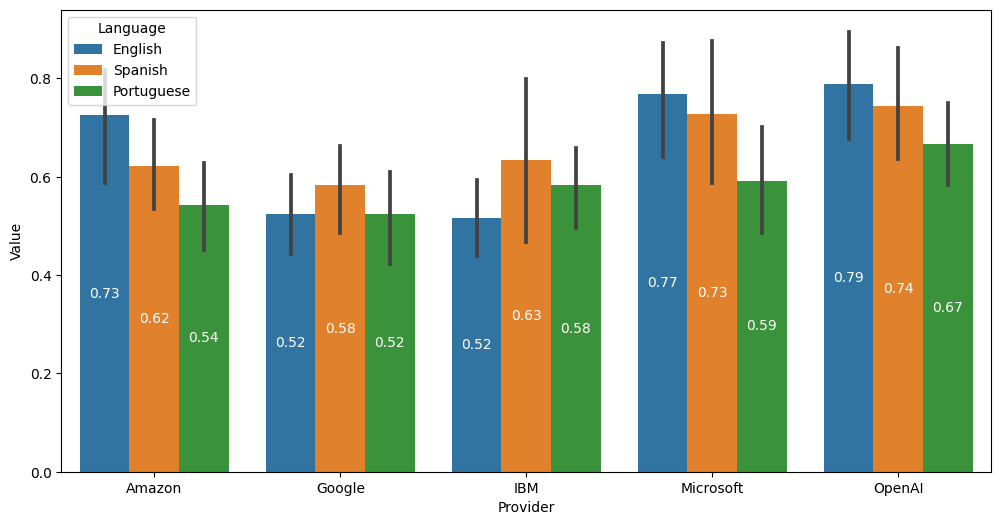
\includegraphics[width=0.9\textwidth]{images/chapter4-cs1-lexical-by-lang-barplot.png}
\fadaptada{FalvoJr2023_HICSS}
\end{figure}

Como resultado, foram identificadas diferenças estatisticamente significativas entre a OpenAI quando comparada com Google e IBM, além da Microsoft quando comparada ao Google. Essas diferenças evidenciam uma variabilidade na eficiência dos provedores ao lidar com a similaridade léxica em diferentes contextos de transcrição automática, sugerindo uma superioridade da OpenAI e da Microsoft tendo em vista suas medidas de Jaccard.

As avaliações estatísticas correspondentes (\autoref{tab:chapter4-results-ji-by-lang-tests}) incluíram testes de normalidade e \textit{One-Way ANOVA} para cada idioma. Os resultados destacaram diferenças significativas em como os provedores geram transcrições automáticas em inglês. Disparidades específicas entre provedores foram detalhadas através de análises \textit{post-hoc}, como \textit{Tukey HSD} e \textit{Bonferroni} para o idioma inglês, indicando que o desempenho pode variar significativamente dependendo do idioma das transcrições.

\begin{table}[htb]
\centering
\caption{Testes Estatísticos do Índice de Jaccard: Provedores Agrupados Por Idioma}
\label{tab:chapter4-results-ji-by-lang-tests} 
\begin{tabular}{|ccccc|}
\hline
\multicolumn{5}{|c|}{\textbf{Tests of Normality}} \\ \hline
\multicolumn{1}{|c|}{\multirow{2}{*}{\textbf{Test}}} & \multicolumn{2}{c|}{\textbf{Kolmogorov-Smirnov}} & \multicolumn{2}{c|}{\textbf{Shapiro-Wilk}} \\ \cline{2-5} 
\multicolumn{1}{|c|}{} & \multicolumn{1}{c|}{\textbf{Statistic}} & \multicolumn{1}{c|}{\textbf{Significance \ensuremath{(p)}}} & \multicolumn{1}{c|}{\textbf{Statistic}} & \textbf{\ensuremath{p}} \\ \hline
\multicolumn{1}{|c|}{EN} & \multicolumn{1}{c|}{0.121} & \multicolumn{1}{c|}{\textbf{0.200}} & \multicolumn{1}{c|}{0.961} & \textbf{0.427} \\ \hline
\multicolumn{1}{|c|}{PT} & \multicolumn{1}{c|}{0.114} & \multicolumn{1}{c|}{\textbf{0.200}} & \multicolumn{1}{c|}{0.942} & \textbf{0.169} \\ \hline
\multicolumn{1}{|c|}{ES} & \multicolumn{1}{c|}{0.951} & \multicolumn{1}{c|}{\textless 0.001} & \multicolumn{1}{c|}{0.951} & \textbf{0.264} \\ \hline
\multicolumn{5}{|c|}{\textbf{One-Way ANOVA}} \\ \hline
\multicolumn{1}{|c|}{\textbf{Test}} & \multicolumn{2}{c|}{\textbf{F}} & \multicolumn{2}{c|}{\textbf{\ensuremath{p}}} \\ \hline
\multicolumn{1}{|c|}{EN} & \multicolumn{2}{c|}{4.88} & \multicolumn{2}{c|}{\textbf{0.007}} \\ \hline
\multicolumn{1}{|c|}{PT} & \multicolumn{2}{c|}{1.058} & \multicolumn{2}{c|}{0.403} \\ \hline
\multicolumn{1}{|c|}{ES} & \multicolumn{2}{c|}{0,931} & \multicolumn{2}{c|}{0,466} \\ \hline
\multicolumn{5}{|c|}{\textbf{Tukey HSD (Honest Significant Difference) - EN}} \\ \hline
\multicolumn{3}{|l|}{\textbf{Providers (Groups from 1 to 5)}} & \multicolumn{2}{c|}{\textbf{\ensuremath{p}}} \\ \hline
\multicolumn{3}{|l|}{OpenAI (Group 5) to Google (Group 2)} & \multicolumn{2}{c|}{\textbf{0.041}} \\ \hline
\multicolumn{3}{|l|}{OpenAI (Group 5) to IBM (Group 3)} & \multicolumn{2}{c|}{\textbf{0.034}} \\ \hline
\multicolumn{5}{|c|}{\textbf{Bonferroni - EN}} \\ \hline
\multicolumn{3}{|l|}{\textbf{Providers (Groups from 1 to 5)}} & \multicolumn{2}{c|}{\textbf{\ensuremath{p}}} \\ \hline
\multicolumn{3}{|l|}{OpenAI (Group 5) to IBM (Group 3)} & \multicolumn{2}{c|}{\textbf{0.047}} \\ \hline
\end{tabular}
\fadaptada{FalvoJr2023_HICSS}
\end{table}

Esses resultados destacam diferenças significativas na qualidade das transcrições automáticas dos provedores avaliados em relação à similaridade léxica. Além disso, abrem caminho para uma exploração mais aprofundada de como essas características podem impactar a experiência do usuário em várias aplicações dessas transcrições. Isso inclui a satisfação do aluno e a percepção sobre a precisão da transcrição em diferentes contextos linguísticos. Tais aspectos são discutidos na subseção seguinte com base nos resultados do \textit{Survey}.

\subsubsection{Respostas do \textit{Survey}}

Com base nos \textit{insights} do estudo de similaridade léxica, esta seção apresenta os resultados de uma pesquisa anônima baseada nas percepções dos participantes sobre a qualidade das transcrições automáticas, explorando o \textit{dataset} definido para as fontes de evidência quantitativas. 

Essa pesquisa teve como objetivo comparar os dados objetivos de similaridade léxica com as avaliações subjetivas de pessoas reais sobre a qualidade das transcrições dos diferentes provedores de serviços de ASR/STT.

Os resultados desta pesquisa foram sintetizados na \autoref{fig:chapter4-cs1-survey-all} para ilustrar as avaliações médias e a distribuição das respostas. O Gráfico de Barras mostra as avaliações médias para cada provedor, com a OpenAI recebendo a maior pontuação, sugerindo uma preferência entre os participantes (\ref{fig:chapter4-cs1-survey-all-barplot}). O Gráfico de Boxplot detalha a dispersão e a tendência central das avaliações para cada provedor, destacando a variação na satisfação dos usuários (\ref{fig:chapter4-cs1-survey-all-boxplot}), enquanto o Gráfico KDE fornece uma estimativa visual da densidade da distribuição das avaliações (\ref{fig:chapter4-cs1-survey-all-kdeplot}).

\begin{figure}[htbp]
\centering
\caption{Respostas do \textit{Survey}: Gráficos dos Provedores Sem Agrupar Por Idioma.}
\label{fig:chapter4-cs1-survey-all}
\begin{subfigure}[b]{0.81\textwidth}
\centering
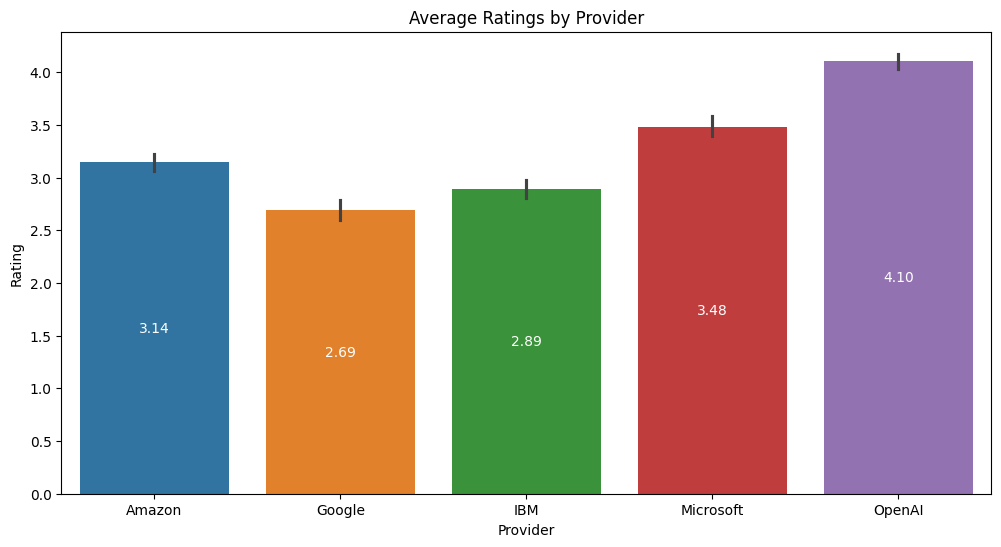
\includegraphics[width=\textwidth]{images/chapter4-cs1-survey-all-barplot.png}
\caption{Gráfico de Barras.}
\label{fig:chapter4-cs1-survey-all-barplot}
\end{subfigure} ~
\begin{subfigure}[b]{0.81\textwidth}
\centering
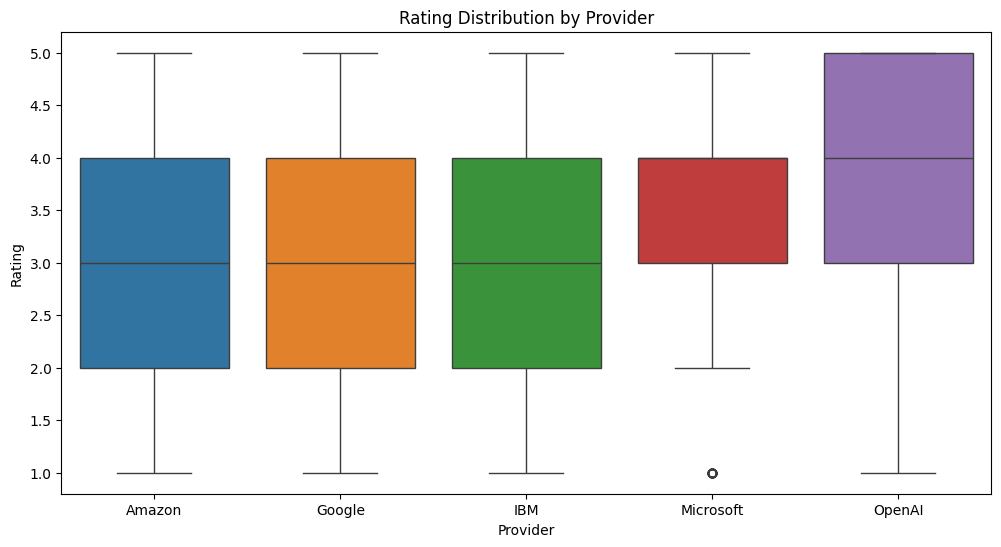
\includegraphics[width=\textwidth]{images/chapter4-cs1-survey-all-boxplot.png}
\caption{Gráfico de Boxplot.}
\label{fig:chapter4-cs1-survey-all-boxplot}
\end{subfigure} ~
\begin{subfigure}[b]{0.81\textwidth}
\centering
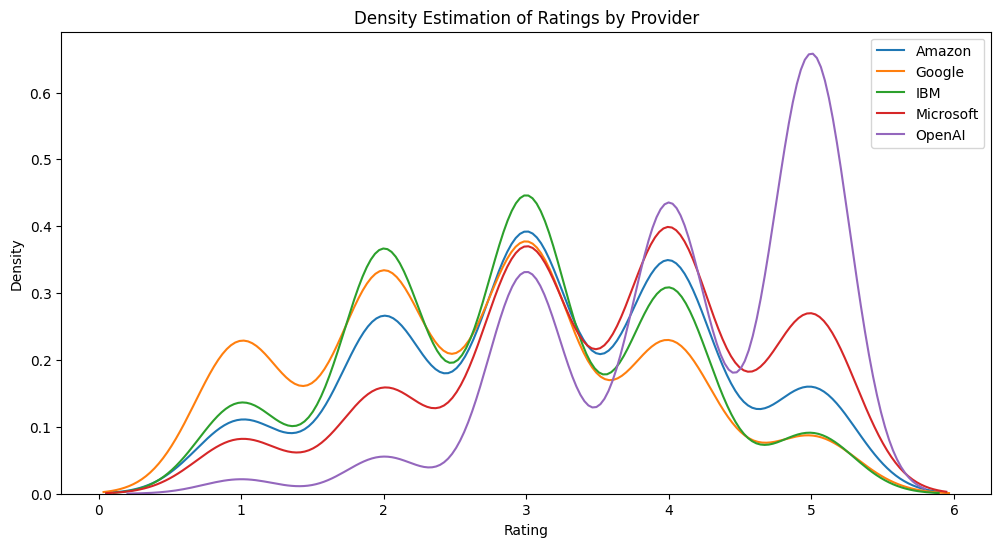
\includegraphics[width=\textwidth]{images/chapter4-cs1-survey-all-kdeplot.png}
\caption{Gráfico KDE.}
\label{fig:chapter4-cs1-survey-all-kdeplot}
\end{subfigure}
\fadaptada{FalvoJr2024_FIE}
\end{figure}

Um gráfico adicional detalha as avaliações por idioma, indicando variações significativas na satisfação do usuário com base no idioma da transcrição automática (\autoref{fig:chapter4-cs1-survey-by-lang-barplot}), o que pode sugerir níveis de qualidade distintos para transcrições em Português, Inglês ou Espanhol.

\begin{figure}[htb]
\centering
\caption{Respostas do \textit{Survey}: Gráfico dos Provedores Agrupados Por Idioma.}
\label{fig:chapter4-cs1-survey-by-lang-barplot}
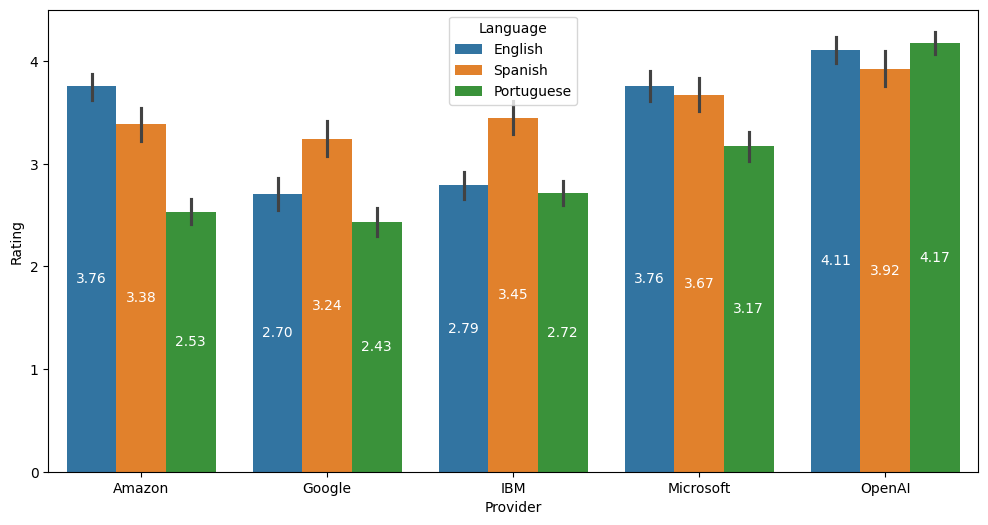
\includegraphics[width=1\textwidth]{images/chapter4-cs1-survey-by-lang-barplot.png}
\fadaptada{FalvoJr2024_FIE}
\end{figure}

As análises estatísticas, consolidadas na \autoref{tab:chapter4-results-survey-tests}, indicaram que as respostas do \textit{Survey} não seguiram uma distribuição normal, característica confirmada pelos testes de \textit{Kolmogorov-Smirnov} \cite{Kolmogorov1933,Smirnov1948} e \textit{Shapiro-Wilk} \cite{Shapiro1965}. Por isso, se fez necessário a avaliação e aplicação de testes não paramétricos para as análises subsequentes. 

O teste de \textit{Kruskal-Wallis} \cite{Kruskal1952}, uma alternativa não paramétrica ao ANOVA, foi empregado para determinar se havia diferenças significativas nas medianas das pontuações entre os diferentes grupos. Este teste mostrou diferenças significativas entre os provedores (\ensuremath{p < 0.05}), sugerindo que as percepções dos participantes variavam significativamente dependendo do provedor.

\begin{table}[htb]
\centering
\caption{Testes Estatísticos do \textit{Survey}: Provedores Sem Agrupar Por Idioma}
\label{tab:chapter4-results-survey-tests} 
\begin{tabular}{|lcccc|}
\hline
\multicolumn{5}{|c|}{\textbf{Tests of Normality}} \\ \hline
\multicolumn{1}{|c|}{\multirow{2}{*}{\textbf{Test}}} & \multicolumn{2}{c|}{\textbf{Kolmogorov-Smirnov}} & \multicolumn{2}{c|}{\textbf{Shapiro-Wilk}} \\ \cline{2-5} 
\multicolumn{1}{|c|}{} & \multicolumn{1}{c|}{\textbf{Statistic}} & \multicolumn{1}{c|}{\textbf{Significance \ensuremath{(p)}}} & \multicolumn{1}{c|}{\textbf{Statistic}} & \textbf{\ensuremath{p}} \\ \hline
\multicolumn{1}{|c|}{Survey Responses} & \multicolumn{1}{c|}{0.887} & \multicolumn{1}{c|}{\textless 0.001} & \multicolumn{1}{c|}{0.973} & \textless 0.001 \\ \hline
\multicolumn{5}{|c|}{\textbf{Interpretation}} \\ \hline
\multicolumn{5}{|l|}{\begin{tabular}[c]{@{}l@{}}Kolmogorov-Smirnov: If \ensuremath{p>0.05}, sample follow the same  statistical distribution.\end{tabular}} \\ \hline
\multicolumn{5}{|l|}{Shapiro-wilk: If \ensuremath{p>0.05} is normal.} \\ \hline
\multicolumn{5}{|c|}{\textbf{Kruskal-Wallis (Non-Parametric equivalent to ANOVA)}} \\ \hline
\multicolumn{1}{|c|}{\textbf{Test}} & \multicolumn{2}{c|}{\textbf{Statistic}} & \multicolumn{2}{c|}{\textbf{\ensuremath{p}}} \\ \hline
\multicolumn{1}{|c|}{Survey Responses} & \multicolumn{2}{c|}{536.167} & \multicolumn{2}{c|}{\textbf{\textless 0.001}} \\ \hline
\multicolumn{5}{|c|}{\textbf{Interpretation}} \\ \hline
\multicolumn{5}{|l|}{\begin{tabular}[c]{@{}l@{}}If \ensuremath{p<0.05}, there are significant differences among the groups.\end{tabular}} \\ \hline
\multicolumn{5}{|c|}{\textbf{Dunn (Non-Parametric Post-Hoc equivalent to Tukey HSB)}} \\ \hline
\multicolumn{3}{|l|}{\textbf{Providers (Groups from 1 to 5)}} & \multicolumn{2}{c|}{\textbf{\ensuremath{p}}} \\ \hline
\multicolumn{3}{|l|}{Amazon (Group 1) to Google (Group 2)} & \multicolumn{2}{c|}{\textbf{\textless 0.001}} \\ \hline
\multicolumn{3}{|l|}{Amazon (Group 1) to IBM (Group 3)} & \multicolumn{2}{c|}{\textbf{\textless 0.001}} \\ \hline
\multicolumn{3}{|l|}{Amazon (Group 1) to Micorsoft (Group 4)} & \multicolumn{2}{c|}{\textbf{\textless 0.001}} \\ \hline
\multicolumn{3}{|l|}{Amazon (Group 1) to OpenAI (Group 5)} & \multicolumn{2}{c|}{\textbf{\textless 0.001}} \\ \hline
\multicolumn{3}{|l|}{Google (Group 2) to IBM (Group 3)} & \multicolumn{2}{c|}{\textbf{0.010}} \\ \hline
\multicolumn{3}{|l|}{Google (Group 2) to Microsoft (Group 4)} & \multicolumn{2}{c|}{\textbf{\textless 0.001}} \\ \hline
\multicolumn{3}{|l|}{Google (Group 2) to OpenAI (Group 5)} & \multicolumn{2}{c|}{\textbf{\textless 0.001}} \\ \hline
\multicolumn{3}{|l|}{IBM (Group 3) to Microsoft (Group 4)} & \multicolumn{2}{c|}{\textbf{\textless 0.001}} \\ \hline
\multicolumn{3}{|l|}{IBM (Group 3) to OpenAI (Group 5)} & \multicolumn{2}{c|}{\textbf{\textless 0.001}} \\ \hline
\multicolumn{3}{|l|}{Micorsoft (Group 4) to OpenAI (Group 5)} & \multicolumn{2}{c|}{\textbf{\textless 0.001}} \\ \hline
\multicolumn{5}{|c|}{\textbf{Interpretation}} \\ \hline
\multicolumn{5}{|l|}{\begin{tabular}[c]{@{}l@{}}If \ensuremath{p<0.05}, it indicates significant pairwise differences between groups.\end{tabular}} \\ \hline
\end{tabular}
\fadaptada{FalvoJr2024_FIE}
\end{table}

Dada a distribuição não normal dos dados, o teste de \textit{Dunn} \cite{Dunn1964} foi escolhido em detrimento do teste de \textit{Conover} \cite{Conover1999} para a análise \textit{post-hoc} devido às suas suposições menos rigorosas sobre a distribuição dos dados e sua capacidade de lidar efetivamente com dados que possuem \textit{outliers} (\autoref{tab:chapter4-results-survey-tests}), embora ambos tenham produzido resultados análogos em testes informais. O teste de \textit{Dunn} comparou pares de provedores, indicando diferenças significativas entre quase todos os pares. Notavelmente, todas as comparações envolvendo OpenAI e outros provedores demonstraram diferenças significativas, sugerindo uma virtual superioridade desse provedor.

Os resultados estratificados por idioma reforçaram essas descobertas, com todos os grupos de idiomas mostrando diferenças significativas entre os provedores na forma como as transcrições automáticas foram avaliadas. Isso sugere que a qualidade percebida pelos participantes não depende apenas do provedor, mas também varia com o idioma, destacando os desafios de fornecer transcrições de alta qualidade de forma uniforme em diferentes contextos linguísticos (\autoref{tab:chapter4-results-survey-by-lang-tests}).

\begin{table}[htb]
\centering
\caption{Testes Estatísticos do \textit{Survey}: Provedores Agrupados Por Idioma}
\label{tab:chapter4-results-survey-by-lang-tests} 
\begin{tabular}{|lcccc|}
\hline
\multicolumn{5}{|c|}{\textbf{Tests of Normality}} \\ \hline
\multicolumn{1}{|c|}{\multirow{2}{*}{\textbf{Test}}} & \multicolumn{2}{c|}{\textbf{Kolmogorov-Smirnov}} & \multicolumn{2}{c|}{\textbf{Shapiro-Wilk}} \\ \cline{2-5} 
\multicolumn{1}{|c|}{} & \multicolumn{1}{c|}{\textbf{Statistic}} & \multicolumn{1}{c|}{\textbf{Significance \ensuremath{(p)}}} & \multicolumn{1}{c|}{\textbf{Statistic}} & \textbf{\ensuremath{p}} \\ \hline
\multicolumn{1}{|c|}{EN} & \multicolumn{1}{c|}{0.897} & \multicolumn{1}{c|}{\textless 0.001} & \multicolumn{1}{c|}{0.897} & \textless 0.001 \\ \hline
\multicolumn{1}{|c|}{PT} & \multicolumn{1}{c|}{0.847} & \multicolumn{1}{c|}{\textless 0.001} & \multicolumn{1}{c|}{0.912} & \textless 0.001 \\ \hline
\multicolumn{1}{|c|}{ES} & \multicolumn{1}{c|}{0.959} & \multicolumn{1}{c|}{\textless 0.001} & \multicolumn{1}{c|}{0.893} & \textless 0.001 \\ \hline
\multicolumn{5}{|c|}{\textbf{Kruskal-Wallis (Non-Parametric)}} \\ \hline
\multicolumn{1}{|c|}{\textbf{Test}} & \multicolumn{2}{c|}{\textbf{Statistic}} & \multicolumn{2}{c|}{\textbf{\ensuremath{p}}} \\ \hline
\multicolumn{1}{|c|}{EN} & \multicolumn{2}{c|}{244.355} & \multicolumn{2}{c|}{\textbf{\textless 0.001}} \\ \hline
\multicolumn{1}{|c|}{PT} & \multicolumn{2}{c|}{355.323} & \multicolumn{2}{c|}{\textbf{\textless 0.001}} \\ \hline
\multicolumn{1}{|c|}{ES} & \multicolumn{2}{c|}{37.615} & \multicolumn{2}{c|}{\textbf{\textless 0.001}} \\ \hline
\multicolumn{5}{|c|}{\textbf{Dunn (Non-Parametric) - EN}} \\ \hline
\multicolumn{3}{|l|}{\textbf{Providers (Groups from 1 to 5)}} & \multicolumn{2}{c|}{\textbf{\ensuremath{p}}} \\ \hline
\multicolumn{3}{|l|}{Amazon (Group 1) to Google (Group 2)} & \multicolumn{2}{c|}{\textbf{\textless 0.001}} \\ \hline
\multicolumn{3}{|l|}{Amazon (Group 1) to IBM (Group 3)} & \multicolumn{2}{c|}{\textbf{\textless 0.001}} \\ \hline
\multicolumn{3}{|l|}{Amazon (Group 1) to OpenAI (Group 5)} & \multicolumn{2}{c|}{\textbf{0.002}} \\ \hline
\multicolumn{3}{|l|}{Google (Group 2) to Microsoft (Group 4)} & \multicolumn{2}{c|}{\textbf{\textless 0.001}} \\ \hline
\multicolumn{3}{|l|}{Google (Group 2) to OpenAI (Group 5)} & \multicolumn{2}{c|}{\textbf{\textless 0.001}} \\ \hline
\multicolumn{3}{|l|}{IBM (Group 3) to Microsoft (Group 4)} & \multicolumn{2}{c|}{\textbf{\textless 0.001}} \\ \hline
\multicolumn{3}{|l|}{IBM (Group 3) to OpenAI (Group 5)} & \multicolumn{2}{c|}{\textbf{\textless 0.001}} \\ \hline
\multicolumn{3}{|l|}{Micorsoft (Group 4) to OpenAI (Group 5)} & \multicolumn{2}{c|}{\textbf{0.005}} \\ \hline
\multicolumn{5}{|c|}{\textbf{Dunn (Non-Parametric) - PT}} \\ \hline
\multicolumn{3}{|l|}{\textbf{Providers (Groups from 1 to 5)}} & \multicolumn{2}{c|}{\textbf{\ensuremath{p}}} \\ \hline
\multicolumn{3}{|l|}{Amazon (Group 1) to Microsoft (Group 4)} & \multicolumn{2}{c|}{\textbf{\textless 0.001}} \\ \hline
\multicolumn{3}{|l|}{Amazon (Group 1) to OpenAI (Group 5)} & \multicolumn{2}{c|}{\textbf{\textless 0.001}} \\ \hline
\multicolumn{3}{|l|}{Google (Group 2) to IBM (Group 3)} & \multicolumn{2}{c|}{\textbf{0.017}} \\ \hline
\multicolumn{3}{|l|}{Google (Group 2) to Microsoft (Group 4)} & \multicolumn{2}{c|}{\textbf{\textless 0.001}} \\ \hline
\multicolumn{3}{|l|}{Google (Group 2) to OpenAI (Group 5)} & \multicolumn{2}{c|}{\textbf{\textless 0.001}} \\ \hline
\multicolumn{3}{|l|}{IBM (Group 3) to Microsoft (Group 4)} & \multicolumn{2}{c|}{\textbf{\textless 0.001}} \\ \hline
\multicolumn{3}{|l|}{IBM (Group 3) to OpenAI (Group 5)} & \multicolumn{2}{c|}{\textbf{\textless 0.001}} \\ \hline
\multicolumn{3}{|l|}{Micorsoft (Group 4) to OpenAI (Group 5)} & \multicolumn{2}{c|}{\textbf{\textless 0.001}} \\ \hline
\multicolumn{5}{|c|}{\textbf{Dunn (Non-Parametric) - ES}} \\ \hline
\multicolumn{3}{|l|}{\textbf{Providers (Groups from 1 to 5)}} & \multicolumn{2}{c|}{\textbf{\ensuremath{p}}} \\ \hline
\multicolumn{3}{|l|}{Amazon (Group 1) to OpenAI (Group 5)} & \multicolumn{2}{c|}{\textbf{\textless 0.001}} \\ \hline
\multicolumn{3}{|l|}{Google (Group 2) to Microsoft (Group 4)} & \multicolumn{2}{c|}{\textbf{0.002}} \\ \hline
\multicolumn{3}{|l|}{Google (Group 2) to OpenAI (Group 5)} & \multicolumn{2}{c|}{\textbf{\textless 0.001}} \\ \hline
\multicolumn{3}{|l|}{IBM (Group 3) to OpenAI (Group 5)} & \multicolumn{2}{c|}{\textbf{\textless 0.001}} \\ \hline
\end{tabular}
\fadaptada{FalvoJr2024_FIE}
\end{table}

A análise da pesquisa efetivamente conecta as medidas objetivas de similaridade léxica e as percepções subjetivas da qualidade das transcrições. A correlação entre as pontuações de similaridade léxica e as excelentes avaliações dos participantes, particularmente para a OpenAI, ressalta a relevância prática da precisão léxica na satisfação dos usuários finais. 

Esses \textit{insights} são fundamentais para provedores que buscam otimizar seus serviços de transcrição para conteúdos educacionais, pois ilustram a importância tanto da precisão linguística quanto da percepção dos usuários finais na avaliação da qualidade das transcrições automáticas. As descobertas sugerem um roteiro para futuras melhorias e a potencial customização de serviços para atender de forma mais eficaz às diversas necessidades linguísticas.

\subsubsection{Pesquisa Documental}

Nesta fase, ampliamos nossa visão sobre as tecnologias de ASR/STT, examinando a literatura para complementar nossas descobertas quantitativas com percepções qualitativas adicionais. Esta análise documental aprofunda-se em diversos estudos que contribuíram significativamente para o campo de ASR e STT, proporcionando uma compreensão mais ampla de como essas tecnologias, impulsionadas por avanços em \textit{Machine Learning} (ML) e AI, podem melhorar a acessibilidade de OAs.

O estudo de \citeonline{Ferraro2023} apresenta uma investigação extensa sobre a transcrição de língua falada usando modelos de ML. Sua análise compara serviços de STT de código aberto e pagos, com foco na qualidade das transcrições automáticas e na diversidade dos dados de entrada. A pesquisa utiliza diversos conjuntos de dados de entrevistas, palestras e discursos, empregando métricas como a Taxa de Erro de Palavras (WER) para avaliação. O trabalho de \citeonline{Ferraro2023} fornece um ponto de referência, alternativo aos métodos de similaridade léxica, para avaliar a precisão da transcrição, estabelecendo uma base sólida para trabalhos futuros.

\citeonline{Bengesi2024} oferecem uma revisão abrangente dos avanços recentes em IAGen, destacando suas aplicações potenciais em processos automáticos de transcrição. Embora não se concentrem diretamente na conversão de fala em texto, sua exploração de modelos de ponta, incluindo Redes Adversárias Generativas (GANs), Transformadores Pré-treinados Generativos (GPT), \textit{autoencoders} e modelos de difusão, fornece uma base para entender como a IAGen pode aprimorar a precisão da transcrição.

\citeonline{Homburg2019} exploram o uso de robôs humanoides como avatares para a tradução de língua de sinais, buscando aprimorar a inclusão da comunidade surda. Diferentemente de pesquisas anteriores, que se concentravam apenas no reconhecimento da língua de sinais, este estudo adota uma abordagem inovadora ao utilizar robôs como intermediários na comunicação. Entrevistando 50 participantes surdos, eles avaliam a eficácia percebida dos robôs humanoides na tradução da língua de sinais, oferecendo \textit{insights} inovadores para soluções de acessibilidade.

\citeonline{Alshaikh2024} exploram a integração da IAGen na educação por meio do desenvolvimento e avaliação de um Assistente de Vídeo Educacional com IA. Fundamentado na Teoria Cognitiva da Aprendizagem Multimídia (CTML), seu ferramental, equipado com módulos de Transcrição, Engajamento e Reforço, utiliza tecnologias ASR para aprimorar a experiência de aprendizagem. Ao focar em experiências de aprendizagem multimodal, seu estudo demonstra o potencial das técnicas avançadas de IA, incluindo STT, para melhorar os resultados educacionais.

\citeonline{Cao2023} abordam as limitações das ferramentas tradicionais de transcrição de áudio em salas de aula ruidosas do mundo real. Sua pesquisa enfatiza o papel crucial de sistemas de aprendizagem inteligentes eficazes em ambientes colaborativos, particularmente na análise e compreensão de conversas entre alunos. Ao explorar a influência dos erros de ASR em modelos de conversação, destacam os desafios e oportunidades para melhorar a precisão do ASR em contextos educacionais.

Com base nas contribuições desses estudos, pretendemos aplicar os princípios da Teoria Fundamentada em Dados \cite{Charmaz2009} para categorizar e analisar os dados qualitativos coletados em nossa pesquisa. A Teoria Fundamentada fornece uma abordagem sistemática para explorar temas emergentes e enriquecer nossa compreensão dos fatores que influenciam a qualidade das transcrições automáticas.

Ao integrar os resultados coletados de nossas fontes de evidência, buscamos identificar padrões e \textit{insights} sobre o uso de tecnologias ASR e STT na melhoria da acessibilidade dos OAs. Para facilitar essa análise, categorizamos os achados de cada estudo dentro da Teoria Fundamentada em temas distintos, permitindo uma compreensão abrangente das implicações tecnológicas e educacionais das ferramentas ASR e STT. Essas categorias incluem:

\begin{itemize}
\item \textbf{Avaliação da Qualidade de Transcrição (AQT)}: Avaliação de desempenho e qualidade em soluções baseadas nas tecnologias de ASR e STT para tarefas de transcrição de fala. Esta categoria foca na precisão das transcrições, utilizando métricas como a Taxa de Erro de Palavras (WER) e comparações entre diferentes serviços de STT, sejam eles de código aberto ou pagos.

\item \textbf{IAGen na Educação (IAGenE)}: Exploração da integração da IAGen em contextos educacionais para aprimorar experiências de aprendizagem. Aqui, a atenção está na aplicação de técnicas de IA, como GANs, GPTs e \textit{autoencoders}, para melhorar processos educacionais, incluindo a transcrição automática de aulas e a personalização da aprendizagem.

\item \textbf{Tecnologias Assistivas (TAs)}: Investigação de abordagens inovadoras, como robôs humanoides e ferramentas de aprendizagem multimodal, para melhorar a acessibilidade para diversos alunos. Esta categoria abrange o uso de TAs para suportar a inclusão de alunos com necessidades especiais, como a tradução/sinalização de línguas de sinais.

\item \textbf{Desafios e Oportunidades (DO)}: Identificação de obstáculos e possibilidades para aprimorar a precisão e eficácia do ASR em contextos educacionais. Este tema envolve os desafios na implementação de tecnologias ASR em ambientes ruidosos e colaborativos, buscando soluções para um reconhecimento de fala assertivo mesmo em situações adversas.
\end{itemize}

Na \autoref{tab:chapter4-grounded-theory-results}, apresentamos a categorização de cada estudo dentro da Teoria Fundamentada, fornecendo uma visão detalhada dos temas abordados em cada estudo e sua relevância para nossos objetivos de pesquisa. Esta análise nos permite estabelecer conexões críticas entre as diferentes vertentes de investigação, revelando como cada estudo contribui para a compreensão das tecnologias ASR e STT em contextos educacionais.

\begin{table}
\centering
\caption{Categorização dos Artigos usando Teoria Fundamentada}
\label{tab:chapter4-grounded-theory-results} 
\begin{tabular}{|c|p{6.8cm}|p{5.7cm}|}\hline
\textbf{Categoria} & \textbf{Descrição} & \textbf{Estudos} \\ \hline
\textbf{AQT} & Avalia o desempenho e qualidade do ASR/STT em tarefas de transcrição. & \citeonline{Ferraro2023} \\ \hline
\textbf{IAGenE} & Explora a integração da IAGen em contextos educacionais. & \citeonline{Bengesi2024,Alshaikh2024} \\ \hline
\textbf{TAs} & Investiga TAs para maior inclusão e acessibilidade na educação. & \citeonline{Homburg2019,Alshaikh2024} \\ \hline
\textbf{DO} & Identifica desafios e oportunidades no ASR/STT em contextos educacionais. & \citeonline{Cao2023} \\  \hline
\end{tabular}
\fadaptada{FalvoJr2024_FIE}
\end{table}

A seguir, vamos discutir a convergência dos dados provenientes das três fontes de evidência investigadas: Métodos de Similaridade Léxica, Respostas do \textit{Survey} e Pesquisa Documental. Ao integrar essas diversas fontes, buscamos uma visão mais robusta sobre o impacto das tecnologias ASR e STT na acessibilidade e eficácia dos OAs. Esta abordagem integrada nos permitirá identificar sinergias e discrepâncias, fornecendo um panorama detalhado e multifacetado dos estados da prática e da arte.

\subsubsection{Convergência de Dados}

Esta pesquisa visa desvendar as complexidades das tecnologias ASR e STT no aprimoramento da acessibilidade dos OAs por meio da triangulação de dados de três fontes distintas. Cada fonte contribui de forma única para uma compreensão abrangente de como a transcrição automática impacta a interação dos alunos com os OAs.

Primeiramente, o uso de métodos de similaridade léxica destacou variações significativas na precisão das transcrições entre os provedores de ASR avaliados (Amazon, Google, IBM, Microsoft, OpenAI). Esses dados elucidaram não apenas as capacidades técnicas desses serviços, mas também ressaltaram as nuances linguísticas que afetam seu desempenho em diferentes idiomas \cite{FalvoJr2023_HICSS}.

Adicionalmente, o \textit{Survey} estende essa análise quantitativa incorporando as percepções dos participantes sobre a qualidade das transcrições. Nesse sentido, as respostas do \textit{Survey} se alinham em alguns aspectos aos resultados da similaridade léxica, reforçando a relevância de uma boa métrica de precisão na satisfação do usuário. No entanto, também evidenciam aspectos centrados no usuário dos serviços de ASR -- como a facilidade de compreensão e a integração com ambientes de aprendizagem -- que não são capturados por algoritmos de similaridade léxica.

Esses dados quantitativos poderosos, baseados na métrica do JI e nas respostas em escala Likert do \textit{Survey}, servem como um aspecto fundamental da nossa triangulação, proporcionando uma linha de base para avaliar a precisão e, consequentemente, a qualidade das transcrições automáticas.

Por sua vez, a pesquisa documental enriquece nossa percepção ao introduzir elementos qualitativos da literatura existente. Esta análise não apenas contextualiza os achados de nossas outras fontes de evidência, mas também explora temas mais amplos, como o impacto educacional das tecnologias de ASR/STT e seu alinhamento com os princípios de acessibilidade. Essa revisão de literatura complementar identificou lacunas e oportunidades interessantes no uso atual do STT, sugerindo áreas para trabalhos futuros tanto no campo tecnológico quanto no pedagógico.

A integração desses três conjuntos de dados -- métodos de similaridade léxica, respostas do \textit{survey} e pesquisa documental -- proporciona uma visão holística sobre o impacto das TICs, como o ASR/STT, na educação. Essa triangulação de dados não apenas confirma a importância da precisão das transcrições, mas também revela a necessidade de uma abordagem centrada no usuário e consciente do contexto para maximizar a eficácia dessas tecnologias. Sendo assim, segue uma síntese da convergência dos dados triangulados:

\begin{itemize}

\item \textbf{Similaridade Léxica vs. Percepções dos Usuários}: Os dados de similaridade léxica revelaram que diferentes provedores de STT têm diferenças estatisticamente significativas na precisão das transcrições. Notavelmente, a OpenAI mostrou um desempenho superior (geral e por idioma) quando comparada a outros provedores de peso como Google e IBM. No entanto, os resultados do \textit{Survey}, que também focaram em avaliações quantitativas, mas usando escala Likert, indicam que a satisfação do usuário é influenciada por mais do que apenas a precisão léxica. Embora a OpenAI também tenha alcançado a maior satisfação entre os participantes, as diferenças estatísticas nas respostas do \textit{Survey} sugerem que as percepções dos usuários são influenciadas por fatores como compreensão do contexto e tolerância a erros, que não são totalmente capturados pelos métodos de similaridade léxica.

\item \textbf{\textit{Insights} Qualitativos da Pesquisa Documental}: A integração da Teoria Fundamentada \cite{Charmaz2009} na nossa análise documental permitiu uma compreensão mais profunda dos temas que afetam a qualidade das transcrições automáticas. Estudos relevantes, como os de \citeonline{Ferraro2023,Alshaikh2024}, enfatizam a importância de considerar tipos de dados diversos e ambientes de aprendizagem ao avaliar tecnologias de ASR/STT. Esses achados sugerem que a eficácia educacional das aplicações de reconhecimento de fala vai além da mera precisão da transcrição, abrangendo a facilidade de integração, as capacidades de personalização e a habilidade da tecnologia de se adaptar às necessidades educacionais diversificadas.

\item \textbf{Contexto Educacional e Acessibilidade/Inclusão}: Os dados triangulados destacam a necessidade de que as tecnologias de ASR/STT se alinhem aos princípios de acessibilidade e inclusividade. As discrepâncias entre a precisão mecânica das transcrições e a satisfação qualitativa dos usuários apontam para uma lacuna nas capacidades atuais do reconhecimento de fala. Essa lacuna indica a necessidade de os provedores inovarem além das métricas tradicionais de precisão e incorporarem \textit{feedback} dos usuários no desenvolvimento de soluções de transcrição mais conscientes do contexto e inclusivas.

\end{itemize}

As convergências identificadas revelam que, embora a precisão léxica das transcrições seja relevante, a satisfação do usuário e a eficácia educacional dependem também de outros fatores, como a facilidade de uso e a capacidade de integração/adaptação a contextos específicos. Este panorama multifacetado sublinha a importância de uma abordagem holística no desenvolvimento e na implementação de tecnologias ASR/STT, conforme as implicações para pesquisas futuras a seguir:

\begin{itemize}
\item \textbf{Aprimoramento do Treinamento de Modelos}: Os achados indicam o potencial de melhorar as tecnologias de ASR/STT treinando modelos em conjuntos de dados linguísticos mais diversos, o que poderia ajudar na compreensão do contexto e na redução de erros nas transcrições automáticas que afetam a satisfação dos usuários finais.

\item \textbf{Customização para Uso Educacional}: Os provedores devem considerar opções de customização que permitam às instituições educacionais adaptar as funcionalidades de ASR/STT às suas necessidades específicas. Alguns exemplos nesse sentido seriam ajustes para diferentes sotaques, dialetos e vocabulário técnico específico de cursos ou disciplinas.

\item \textbf{Abordagens de Design Centrado no Usuário}: Incorporar \textit{feedback} dos usuários no processo de desenvolvimento pode garantir que as futuras melhorias nas tecnologias de ASR/STT estejam mais alinhadas com as necessidades e expectativas dos usuários finais, particularmente em ambientes educacionais diversificados.

\end{itemize}

A convergência dos dados da análise léxica, dos \textit{surveys} dos usuários e da pesquisa acadêmica pinta um quadro complexo do estado atual e do potencial das tecnologias de ASR/STT na educação. Embora avanços notáveis em precisão de transcrição tenham sido alcançados, ainda há um trabalho significativo a ser feito para realizar plenamente o potencial dessas tecnologias em melhorar a acessibilidade e inclusão educacional.

Sendo assim, pesquisas futuras podem se concentrar em fechar a lacuna entre a proficiência técnica e a satisfação do usuário, enfatizando o desenvolvimento de sistemas adaptáveis, amigáveis ao usuário e conscientes do contexto que possam suportar uma ampla gama de ambientes e necessidades de aprendizagem.

Seguindo esta linha de investigação, o próximo estudo de caso explorará a PoC implementada no primeiro estudo de caso para acelerar o desenvolvimento de um player de vídeo aderente ao conceito de Design Universal. Esta PoC se aproveita das transcrições e legendas para integrar o player com avatares de Libras baseados em texto, ampliando ainda mais a acessibilidade e a inclusão em ambientes educacionais.

\section{Estudo de Caso 2: Player com Avatar de Libras}

Nosso segundo estudo de caso concentrou-se no desenvolvimento de um player de vídeo, projetado com base no conceito de Design Universal para criar um produto final mais flexível e acessível do ponto de vista educacional \cite{GovBr2023}. Este estudo também foi conduzido com o apoio da DIO, explorando a API REST desenvolvida como PoC no primeiro estudo de caso para acesso às videoaulas da \textit{EdTech}. Na prática, a integração com a API permite que este player utilize o reconhecimento de fala como um componente central para tornar seus OAs mais inclusivos.

A relevância deste estudo está em sua capacidade de explorar a eficácia e o impacto de avatares de Libras baseados em texto na acessibilidade educacional para a comunidade surda. Para isso, conduzimos avaliações qualitativas através de entrevistas com intérpretes de Libras, investigando como essa solução tecnológica pode melhorar a acessibilidade a OAs audíveis.

\subsection{Prova de Conceito: Player de Vídeo com Design Universal}

A \autoref{fig:chapter4-cs2-poc-diagram} ilustra, por meio de um diagrama de sequência, a dinâmica do player de vídeo desenvolvido, que utiliza as capacidades da arquitetura \textit{Speech2Learning} para ampliar a acessibilidade de videoaulas. Esta representação demonstra como o player de vídeo promove novas formas de explorar OAs audíveis, aproveitando os metadados fornecidos pela API desenvolvida anteriormente.

\begin{figure}[htbp]
\centering
\caption{Visão 2ª Instância da \textit{Speech2Learning}: Player de Vídeo com Avatar de Libras}
\label{fig:chapter4-cs2-poc-diagram}
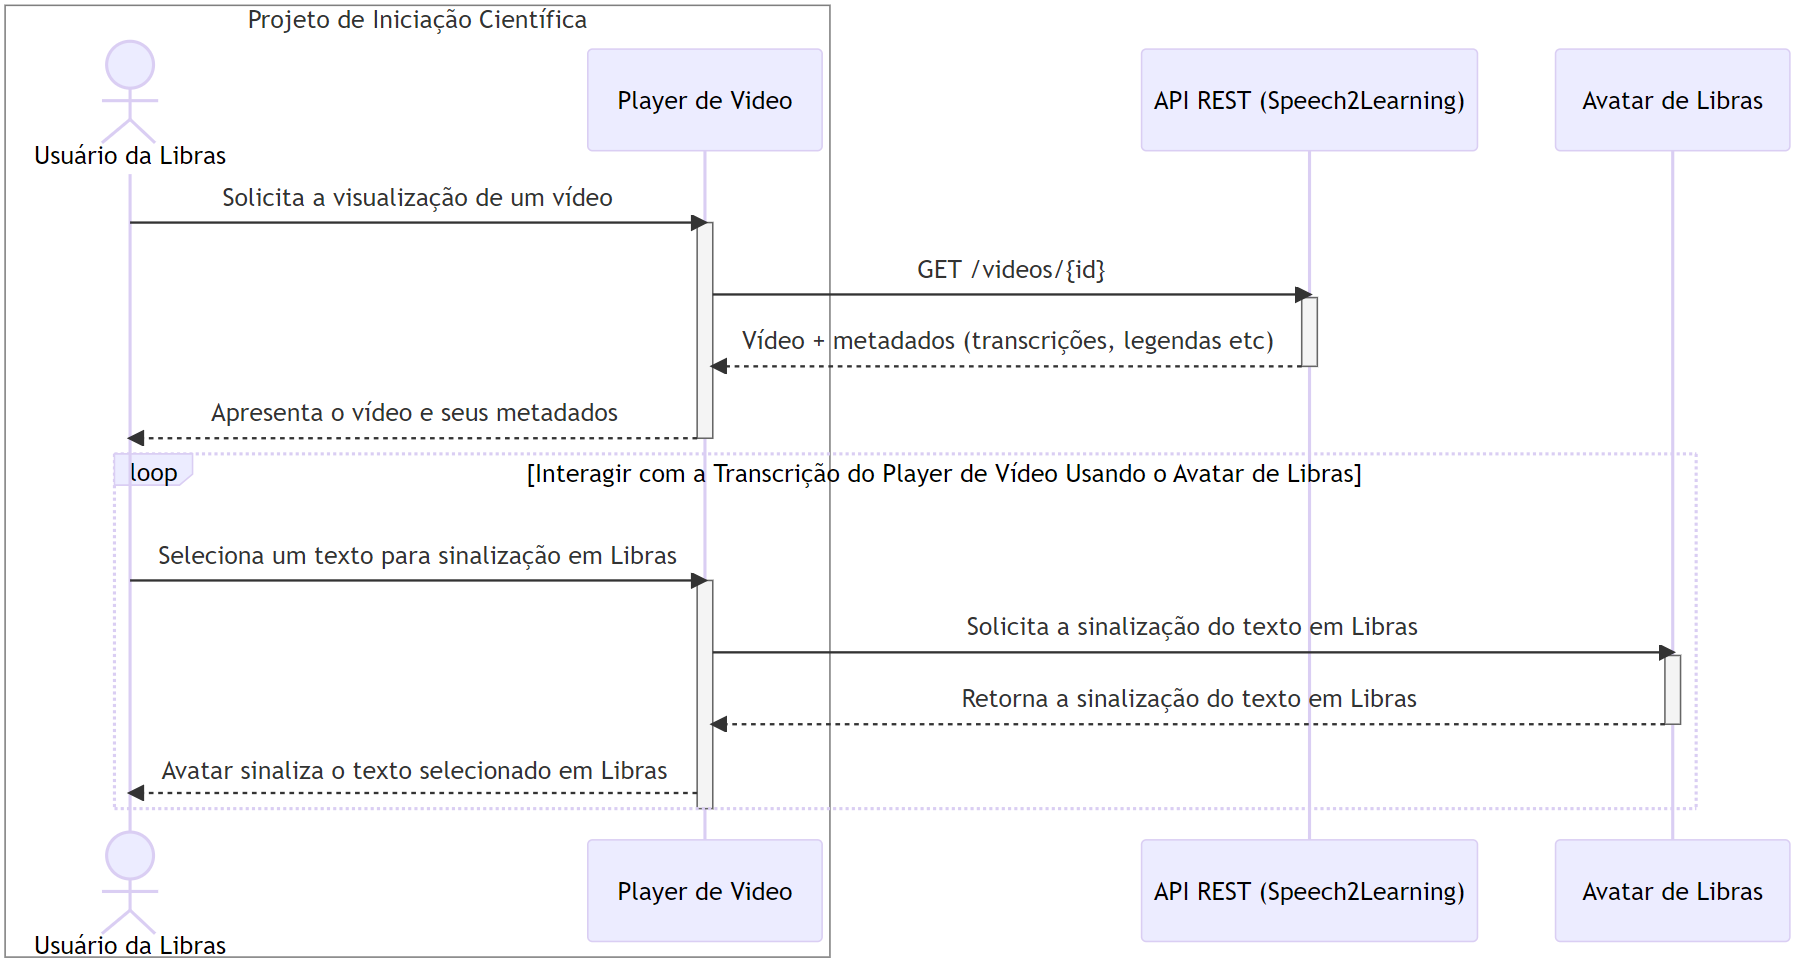
\includegraphics[width=.94\textwidth]{images/chapter4-cs2-poc-diagram.png}
\end{figure}

A integração entre o player de vídeo e a API REST ilustra a capacidade da arquitetura \textit{Speech2Learning} de fomentar ambientes educacionais mais inclusivos. Adotando esta abordagem, os desenvolvedores podem criar sistemas robustos, tecnologicamente independentes e flexíveis, capazes de atender às especificidades de cada projeto.

O objetivo central deste estudo é projetar, implementar e avaliar um player de vídeo que siga as recomendações do ``Guia de Boas Práticas para Acessibilidade Digital'' definidas por \citeonline{GovBr2023} e os princípios de Design Universal promovidos pela \citeonline{UNESCO2023}. Este player, integrado com a arquitetura \textit{Speech2Learning}, visa promover a educação inclusiva para surdos através da Libras.

Tecnicamente, o player foi implementado utilizando HTML, CSS e JavaScript de forma ``pura'' (\textit{vanilla}), ou seja, evitando bibliotecas e/ou implementações alternativas para uma solução mais padronizada e manutenível baseada na Web \cite{GovBr2023}. Os \textit{wireframes} preliminares na Figura \ref{fig:chapter4-cs2-poc-wireframes} oferecem uma visão simplificada, destacando características universais e o símbolo ``Acessível em Libras'', sublinhando o compromisso com a educação inclusiva.

\begin{figure}[htbp]
\centering
\caption{\textit{Wireframes} do Player de Vídeo Acessível (Modos Claro e Escuro)}
\label{fig:chapter4-cs2-poc-wireframes}
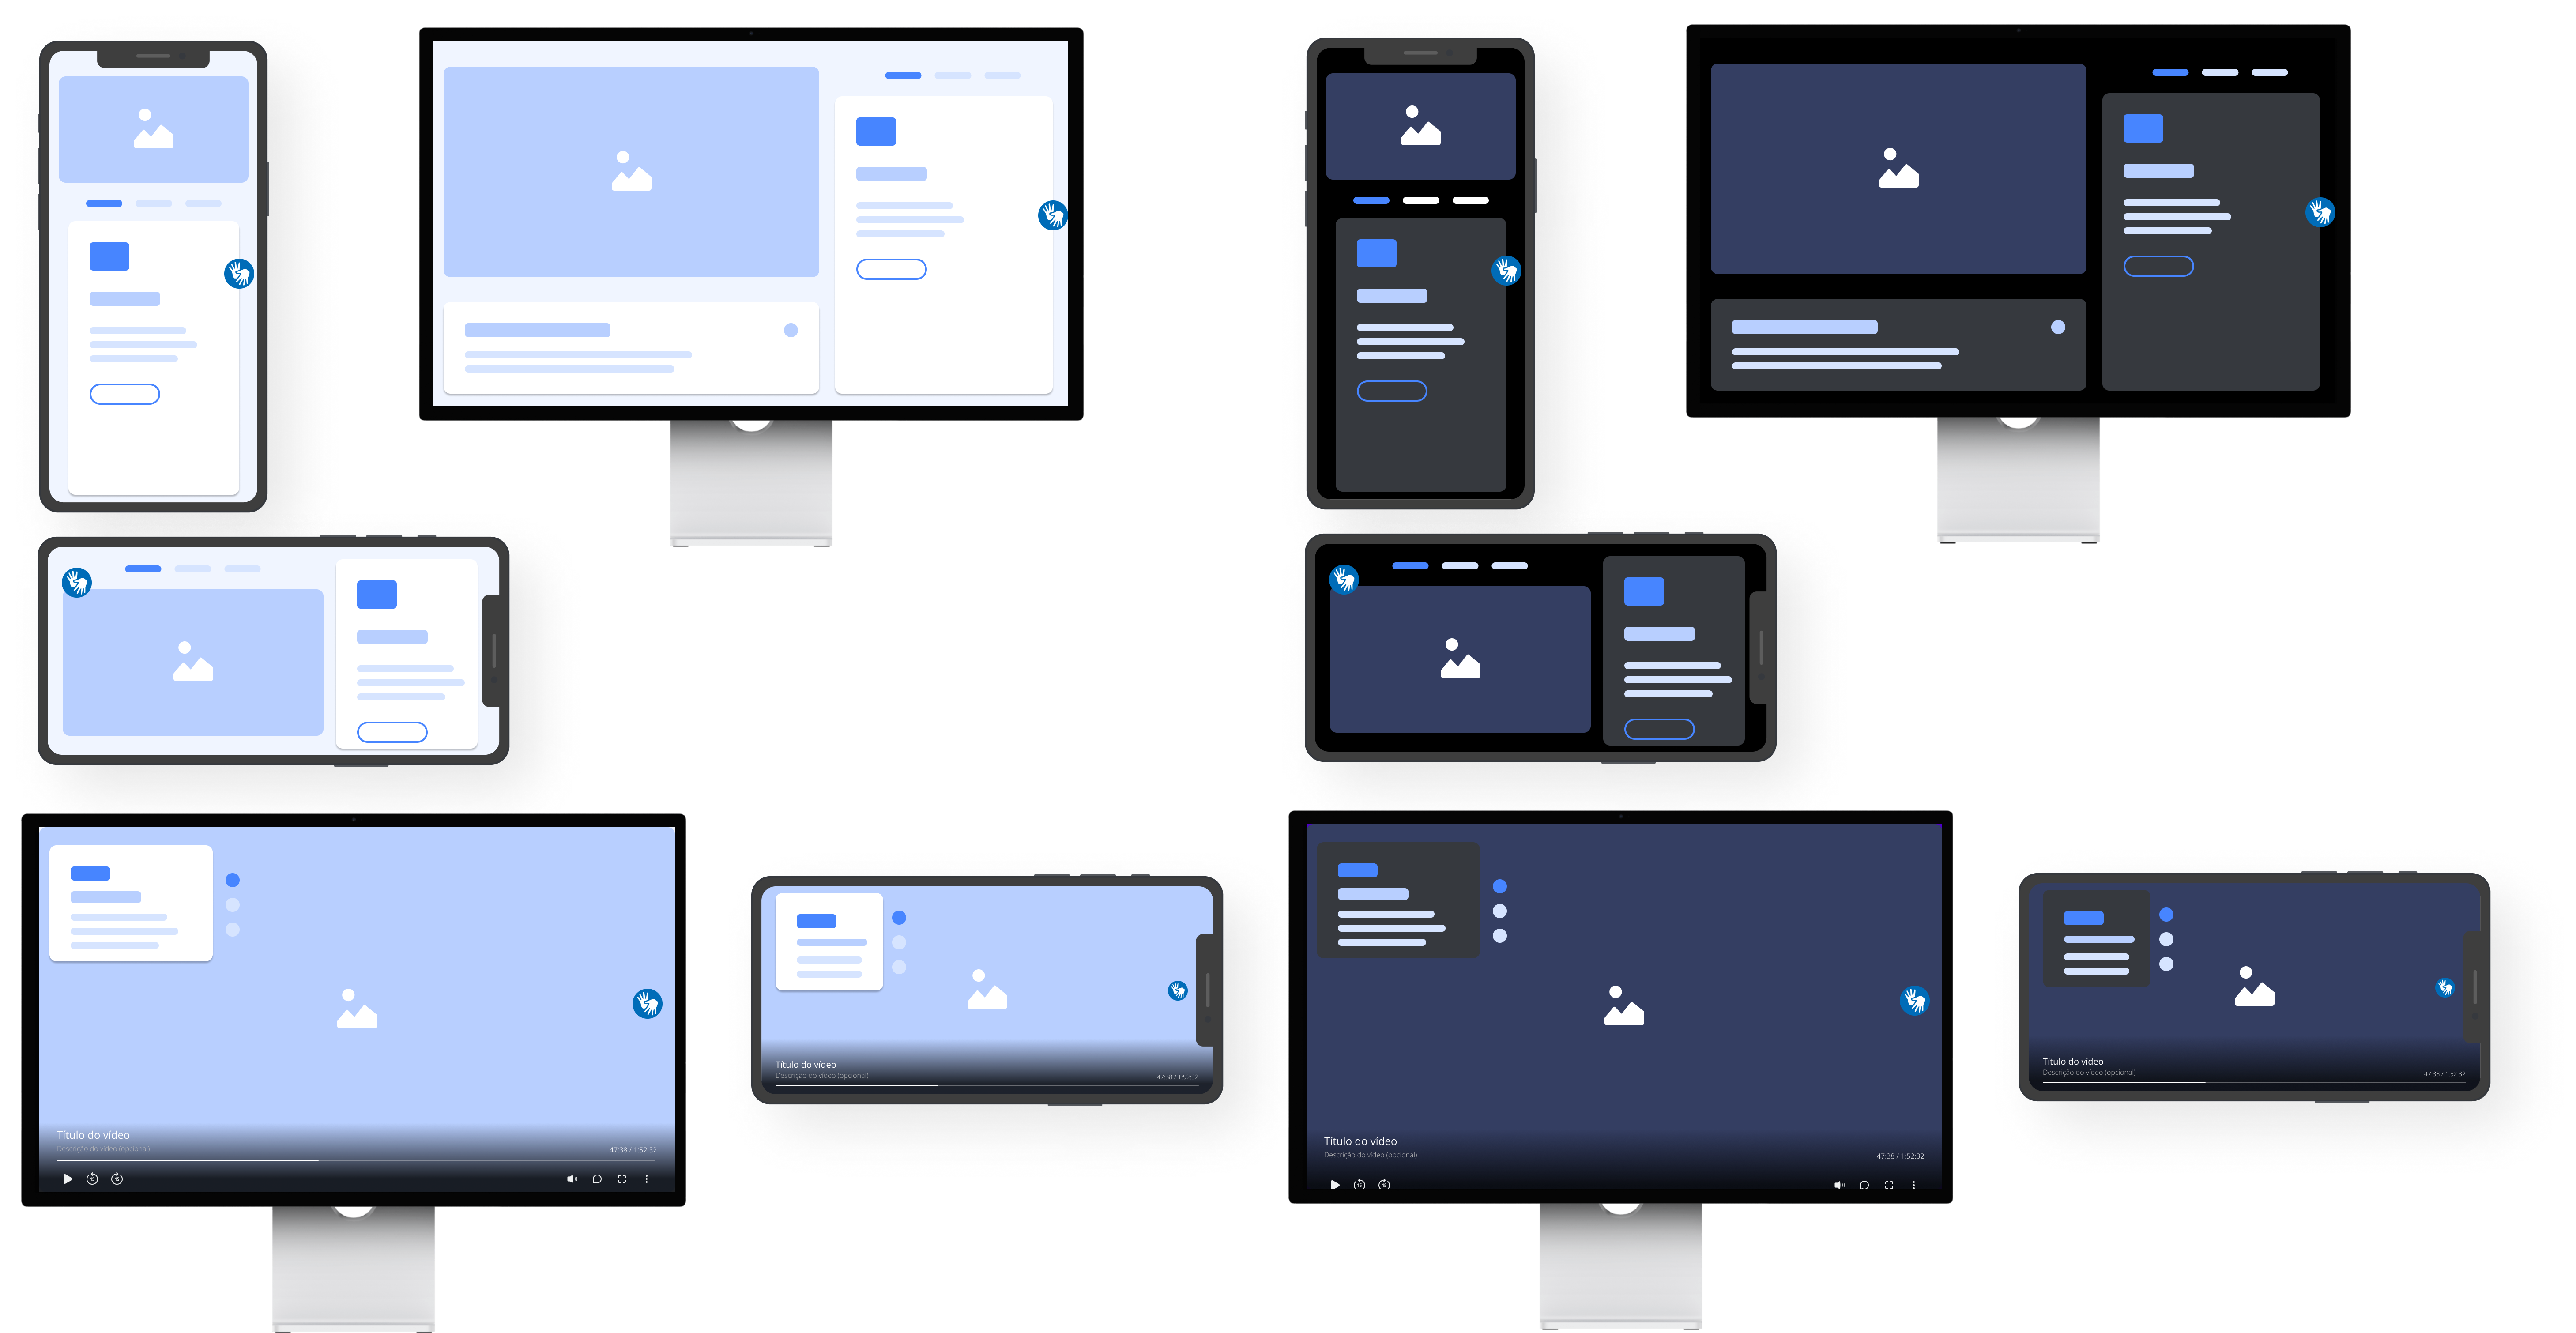
\includegraphics[width=1\textwidth]{images/chapter4-cs2-poc-wireframes.png}
\end{figure}

Em particular, esta PoC contou com dois projetos de Iniciação Científica (IC), um com foco no desenvolvimento do Design Universal da solução e outro na implementação da mesma como uma biblioteca flexível e aberta.

Sendo assim, fez-se necessário o uso de um processo de desenvolvimento de software para que as entregas fossem previsíveis e devidamente validadas. Para isso, seguimos uma metodologia ágil, com ritos simplificados e \textit{Sprints} de duas semanas.

\subsection{Metodologia}

Para investigar o impacto e a eficácia do player de vídeo com avatares de Libras baseados em texto, adotamos uma perspectiva exploratória, caracterizada pela elaboração de conhecimentos ou levantamento de informações sobre um fenômeno ainda pouco conhecido \cite{CastroFilho2021}. Este estudo de caso visa atingir dois principais objetivos: (i) investigar o impacto de avatares de Libras na acessibilidade de conteúdos para surdos; e (ii) explorar a eficácia desses avatares integrados à transcrição automática de videoaulas para a compreensão de OAs audíveis. 

Para alcançar esses objetivos, formulamos a seguinte questão de pesquisa, que é similar à que orientou nossa análise documental, mas com foco em usuários da Libras, incluindo principalmente a comunidade surda:

\begin{itemize}
    \item \textbf{Questão de Pesquisa}: Como as tecnologias de reconhecimento de fala (ASR/STT) podem contribuir para uma educação mais acessível para usuários da Libras?
\end{itemize}

A metodologia empregada foi predominantemente qualitativa, utilizando dados coletados através de entrevistas semi-estruturadas com intérpretes de Libras. Esses dados qualitativos foram fundamentais para compreender as percepções dos intérpretes sobre a precisão, usabilidade e impacto dos avatares de Libras integrados a transcrições automáticas de videoaulas.

A principal fonte de dados para este estudo foram entrevistas qualitativas com intérpretes de Libras. As entrevistas foram cuidadosamente planejadas e conduzidas para explorar profundamente as percepções e experiências dos intérpretes ao utilizar o player de vídeo com avatares de Libras. A coleta de dados seguiu um protocolo estruturado, assegurando que todas as áreas relevantes fossem abordadas durante as entrevistas.

A análise dos dados foi conduzida utilizando a TFD \cite{Charmaz2009}, uma metodologia que possibilita o desenvolvimento de teorias emergentes diretamente dos dados. Este processo iterativo envolveu a codificação aberta para identificar e categorizar os principais temas nas respostas dos intérpretes de Libras. A abordagem garantiu que os temas e padrões emergissem dos dados, proporcionando uma compreensão aprofundada das percepções e experiências dos participantes sem a imposição de noções preconcebidas.

Esperamos que esta segunda instância da arquitetura \textit{Speech2Learning}, através do uso de um player de vídeo acessível com avatares de Libras, melhore significativamente a acessibilidade de conteúdos educacionais para alunos surdos. Este estudo visa demonstrar que tal solução tecnológica pode:

\begin{itemize}
    \item Ampliar de maneira significativa o acesso à OAs audíveis para alunos surdos, fornecendo uma TA que potencializa a inclusão por meio do conceito de ASR, intrínseco em soluções baseadas na arquitetura \textit{Speech2Learning}.
    \item Mostrar a viabilidade e precisão dos avatares de Libras como TA, complementando as estratégias existentes de acessibilidade presentes nas premissas de Design Universal, por exemplo.
    \item Fornecer \textit{insights} valiosos sobre as preferências dos intérpretes de Libras e suas percepções sobre a usabilidade, precisão e impacto dos avatares integrados à transcrições automáticas na educação para surdos.
\end{itemize}

Para concluir, a síntese da \autoref{tab:chapter4-cs2-summary} resume a abordagem metodológica adotada, destacando a importância das entrevistas qualitativas para a compreensão das percepções dos intérpretes de Libras. A análise qualitativa proporcionou uma visão detalhada dos desafios e benefícios percebidos na utilização de avatares de Libras, contribuindo para o desenvolvimento de práticas pedagógicas mais inclusivas e acessíveis.

\begin{table}[htb]
\centering
\caption{Síntese do Estudo de Caso 2: Player de Vídeo com Avatar de Libras}
\label{tab:chapter4-cs2-summary}
\begin{tabular}{|C{3cm}|m{11.75cm}|}\hline
\textbf{Objeto de Estudo} & Player de Vídeo com Avatar de Libras Baseado em Texto (Transcrição Automática) \\\hline
\textbf{Perspectiva} & Exploratório \\\hline
\textbf{Característica} & Elaboração de conhecimentos ou levantamento de informação acerca do fenômeno ainda pouco conhecido \cite{CastroFilho2021}. \\\hline
\textbf{Objetivos} & \begin{tabular}[c]{@{}m{11.75cm}@{}}1. Investigar o impacto de avatares de Libras baseados em texto na acessibilidade de conteúdos para surdos. \\ 2. Explorar a eficácia de avatares de Libras integrados à transcrição automática de videoaulas para a compreensão de OAs audíveis.\end{tabular} \\\hline
\textbf{Questões de Pesquisa} & Como as tecnologias de reconhecimento de fala (ASR/STT) podem contribuir para uma educação mais acessível para usuários da Libras? \\\hline
\textbf{Hipóteses} & Não aplicável \\\hline
\textbf{Fontes de Dados} & Dados qualitativos de entrevistas com intérpretes de Libras. \\\hline
\textbf{Método de Coleta de Dados} & Entrevistas semi-estruturadas \\\hline
\textbf{Tipo de Análise} & Qualitativa \\\hline
\end{tabular}
\end{table}

\subsection{Resultados e Discussões}

Os estudos de caso desta tese de doutorado foram aprovados pelo \sigla{CEP}{Comitê de Ética e Pesquisa}, sob o CAAE 78381524.3.0000.5390. É importante destacar que, embora ambos os estudos tenham sido descritos no projeto submetido ao CEP, o foco principal foi no Estudo de Caso 2, devido à realização de entrevistas com intérpretes de Libras e sua natureza qualitativa. Por outro lado, o Estudo de Caso 1, centrado majoritariamente em análises quantitativas da precisão de transcrições automáticas, não necessitou de uma submissão individual para avaliação ética devido às suas características.

Atualmente, as entrevistas estão sendo agendadas e conduzidas com os intérpretes de Libras da QS Inclusão (\url{https://qsinclusao.com.br}). Embora os resultados ainda não tenham sido totalmente analisados e estratificados para discussões mais aprofundadas, o roteiro completo para as entrevistas com os intérpretes está disponível no \autoref{appendix:interview-form}.

Na prática, tendo em vista o nosso planejamento e previsão financeira, utilizamos apenas o \textit{VLibras} como avatar de Libras. Ele foi priorizado em detrimento ao \textit{Hand Talk} por ser gratuito, \textit{open-source} e mantido pelo governo brasileiro. Além disso, possui configurações avançadas relacionadas à regionalidade e, nos últimos anos, voltou a ser atualizado com frequência.

Algo interessante, que se alinha com esta seção, foi que tivemos a oportunidade de apresentar uma demonstração do nosso player de vídeo (\autoref{fig:chapter4-cs2-poc-demo}) no ``\textit{Workshop on Opportunities and Challenges of Generative AI in Education}'' da ``\textit{57th Hawaii International Conference on System Sciences}'' (HICSS). Seguem algumas dúvidas e feedbacks relevantes deste evento:

\begin{figure}[htbp]
\centering
\caption{\textit{Screenshots} da Demo do Player Apresentada no HICSS.}
\label{fig:chapter4-cs2-poc-demo}
\begin{subfigure}[b]{0.83\textwidth}
\centering
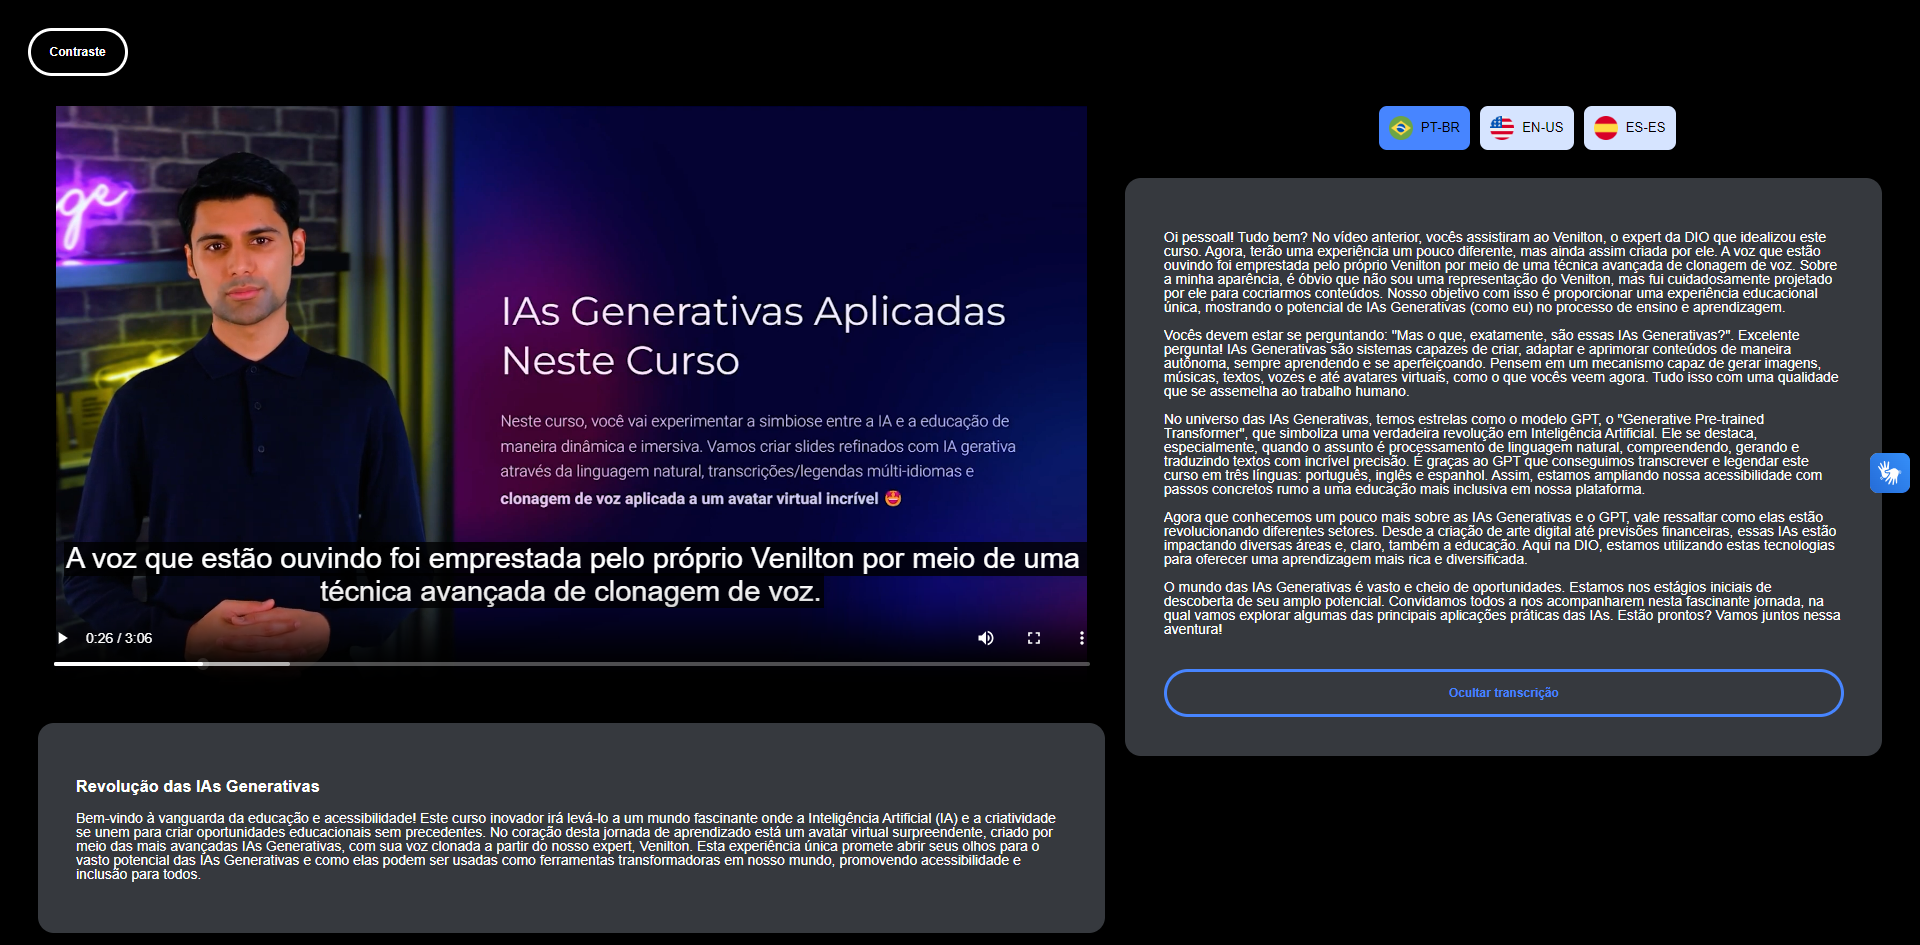
\includegraphics[width=\textwidth]{images/chapter4-cs2-poc-demo1.png}
\caption{Player de Vídeo: Transcrições e Legendas.}
\label{fig:chapter4-cs2-poc-demo1}
\end{subfigure} ~
\begin{subfigure}[b]{0.83\textwidth}
\centering
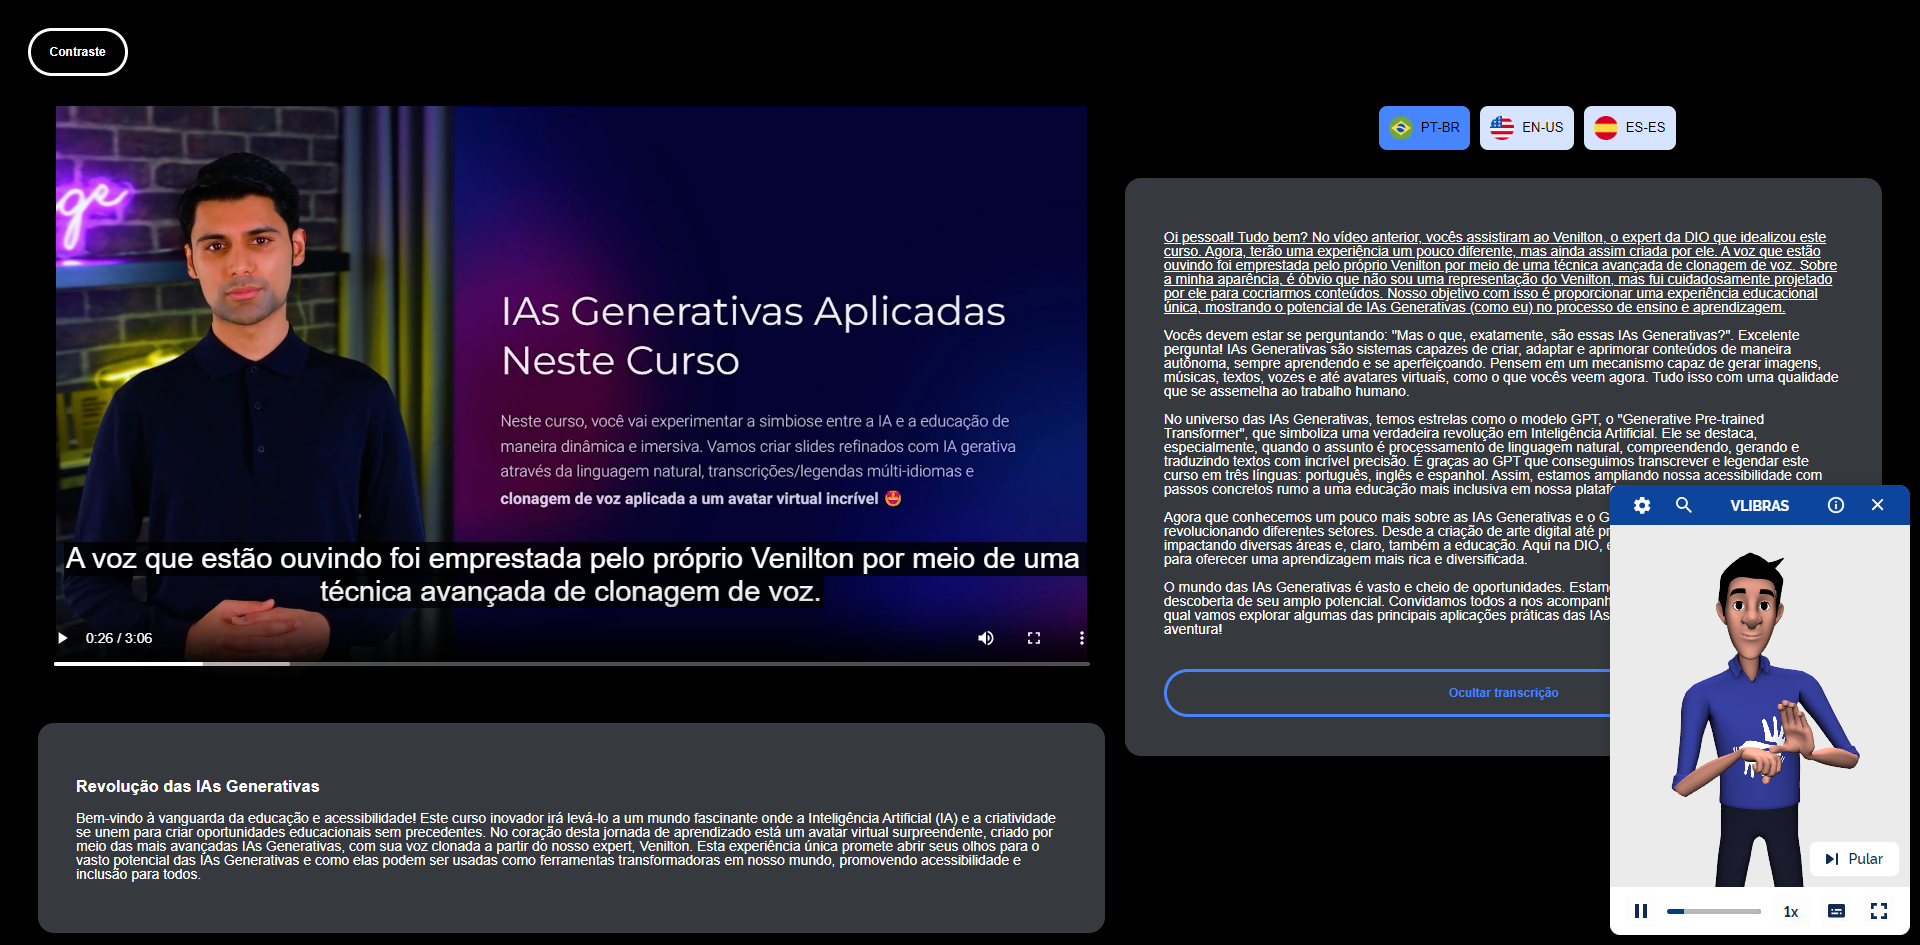
\includegraphics[width=\textwidth]{images/chapter4-cs2-poc-demo2.png}
\caption{Player de Vídeo: Avatar de Libras (VLibras) Sinalizando.}
\label{fig:chapter4-cs2-poc-demo2}
\end{subfigure} ~
\begin{subfigure}[b]{0.83\textwidth}
\centering
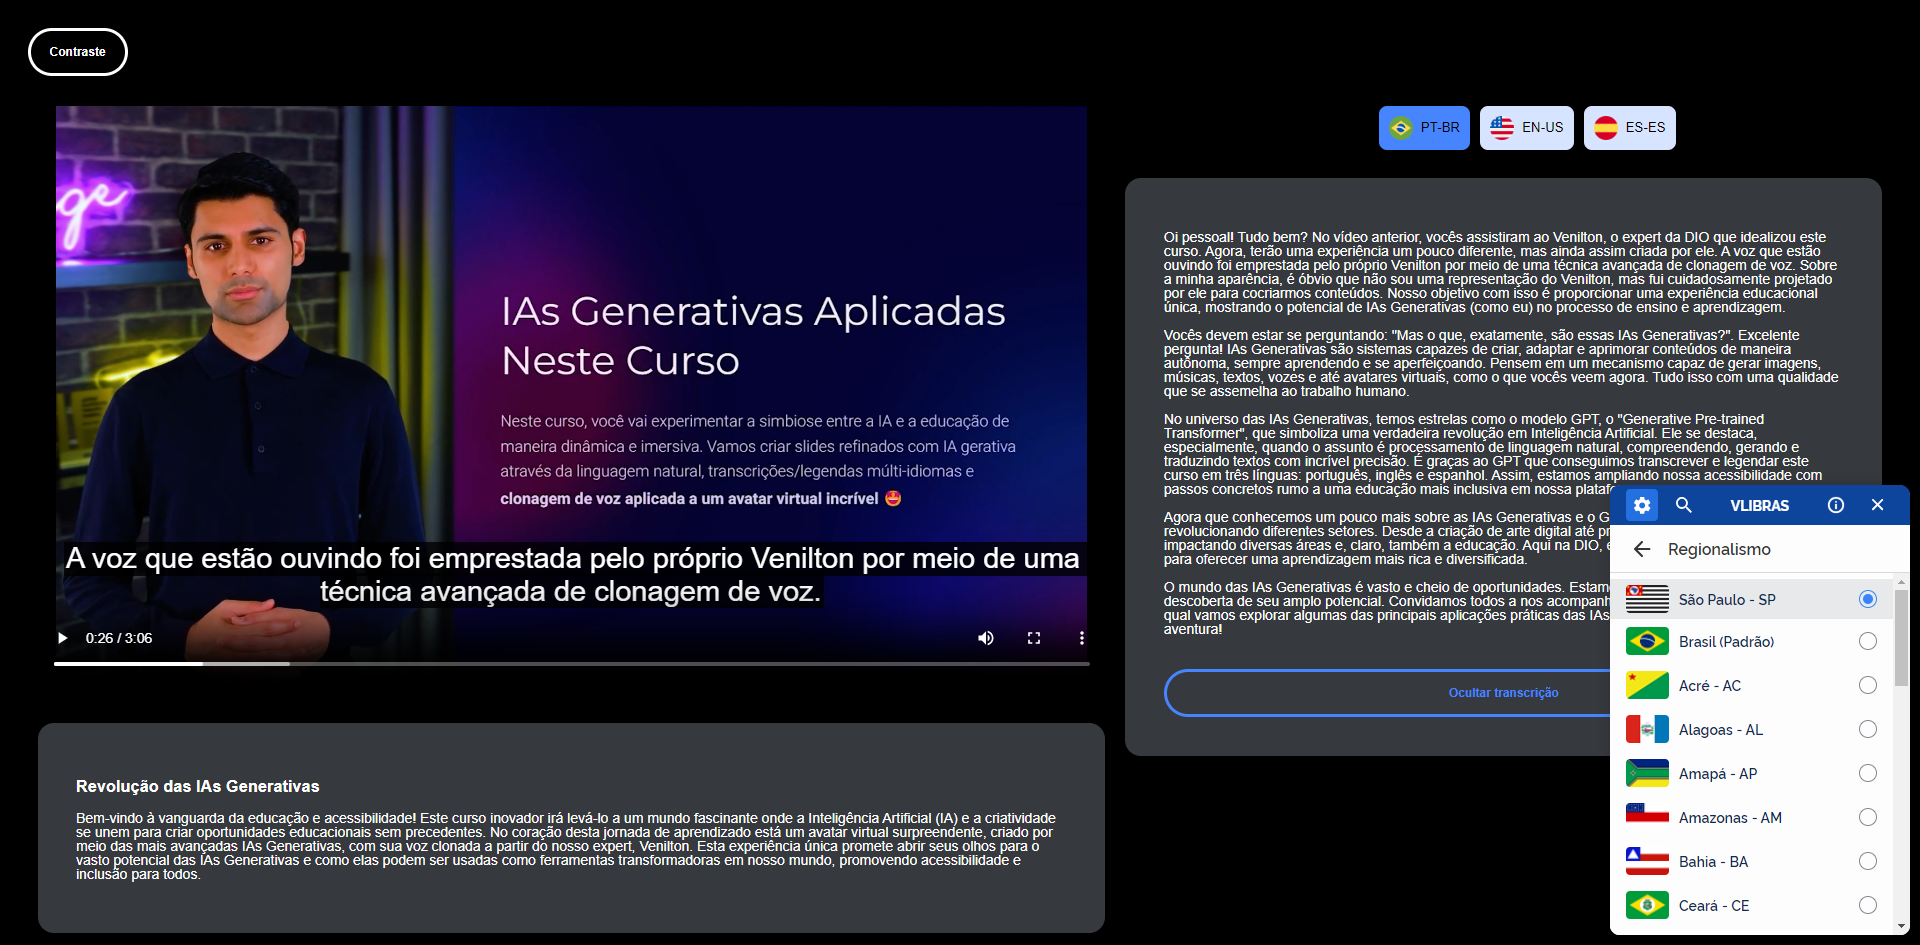
\includegraphics[width=\textwidth]{images/chapter4-cs2-poc-demo3.png}
\caption{Player de Vídeo: Avatar de Libras (VLibras) Regionalismo.}
\label{fig:chapter4-cs2-poc-demo3}
\end{subfigure}
\fautor
\end{figure}

\begin{itemize}
    \item \textbf{Como lidar com as variações regionais das próprias línguas de sinais?}
    É fundamental reconhecer a importância das regionalidades e sotaques tanto na língua falada quanto na sinalizada. A variação regional é uma característica intrínseca das línguas de sinais, que varia conforme a localização geográfica. Em nosso estudo, utilizamos o \textit{VLibras}, que possui configurações de regionalidade para cada estado do Brasil, garantindo que o avatar considere essas variações ao sinalizar. Este aspecto é crucial para a aceitação e eficácia do avatar de Libras, pois respeita as particularidades culturais e linguísticas dos usuários.
    \item \textbf{Qual seria o esforço para integrar o Player de Vídeo a avatares de outras línguas de sinais, como a ASL?}
    Nosso player foi implementado seguindo as práticas de Design Universal, que preconizam que as soluções atendam ao maior número possível de usuários. O player é, essencialmente, uma biblioteca HTML, CSS e JavaScript, garantindo que o player de vídeo HTML, bem como sua descrição, transcrições e legendas, sigam as boas práticas de semântica, estilos e interações. Dessa forma, o player não precisa "conhecer" o avatar de língua de sinais específico, pois está preparado estruturalmente para integrá-lo, facilitando a adaptação para outras línguas de sinais, como a ASL.
    \item \textbf{Como as IAGen estão ajudando no desenvolvimento de projetos relacionados à Arquitetura Speech2Learning?}
    Os modelos de ML têm evoluído consideravelmente nos últimos anos, e hoje é comum ouvirmos falar de GPT e outras siglas comuns na IA. As tecnologias de ASR e STT têm se beneficiado muito dessa revolução. O modelo de reconhecimento de fala da OpenAI, por exemplo, chamado Whisper, é baseado na ideia de \textit{Transformers}, a mesma tecnologia subjacente ao ChatGPT. Notavelmente, o Whisper se destacou em nossos testes e análises estatísticas, e foi escolhido como provedor padrão em nossa API de transcrição e legendagem de videoaulas devido à sua precisão e confiabilidade.
\end{itemize}

Em síntese, nosso estudo de caso sobre o Player de Vídeo com Avatar de Libras demonstra um avanço significativo na inclusão educacional para alunos surdos. A implementação da arquitetura \textit{Speech2Learning} com o uso de avatares de Libras, como o VLibras, potencializa a acessibilidade de conteúdos educacionais, respeitando as particularidades regionais e culturais dos usuários. A apresentação e os feedbacks recebidos no HICSS reforçam a relevância e a aplicabilidade de nossa solução, destacando a importância de continuar explorando e aperfeiçoando tecnologias assistivas no contexto educacional.

\section{Considerações Finais}

Os dois estudos de caso apresentados nesta seção demonstram a importância e a viabilidade de utilizar tecnologias de reconhecimento de fala para promover a inclusão educacional. No primeiro estudo de caso, focado em legendas automáticas para videoaulas, comprovamos que transcrições automáticas precisas podem aumentar significativamente o potencial de acessibilidade em OAs audíveis. No segundo estudo de caso, o desenvolvimento de um player de vídeo com Design Universal, integrado com transcrições automáticas de videoaulas, mostrou-se uma solução promissora para atender às necessidades específicas da comunidade surda, oferecendo uma TA flexível e compatível com avatares de Libras baseados em texto.

Os resultados obtidos até o momento indicam que a integração de tecnologias como ASR/STT com soluções educacionais pode proporcionar uma educação mais inclusiva e acessível. A continuidade deste trabalho incluirá a análise detalhada dos dados coletados nas entrevistas com intérpretes de Libras. Além disso, futuras pesquisas poderão explorar a adaptação de avatares de outras línguas de sinais e o uso de novas tecnologias de IA para aprimorar ainda mais as soluções desenvolvidas.

Em conclusão, os estudos de caso apresentados nesta tese representam um avanço significativo na direção de uma educação verdadeiramente acessível a todos. A aplicação da arquitetura \textit{Speech2Learning} e o uso de avatares de Libras destacam-se como abordagens inovadoras e eficazes para promover a inclusão educacional, contribuindo para a construção de um ambiente educacional mais justo e igualitário.


\chapter{Conclusões}
\label{chapter5}

\noindent
\textcolor{red}{
Dúvidas e Pendências:
\begin{itemize}
    \item TODO: Padronizar as Tabelas e Figuras em Português ou Inglês?
    \item TODO: \textit{Screenshots} da DIO no Estudo de Caso 1: Videoaulas com Legendadas?
    \item TODO: Retomar as Hipóteses e QPs nos Resultados dos Estudos de Caso ou na Conclusão?
    \item TODO: Incluir os Formulários/Surveys como Apêndices (como fiz com a Entrevista)?
\end{itemize}
}

\section{Contribuições da Pesquisa}

\section{Limitações da Pesquisa}

\section{Trabalhos Futuros}

\section{Publicações Resultantes}

As principais publicações resultantes das atividades conduzidas nesta pesquisa de doutorado são apresentadas a seguir, ordenadas cronologicamente:

\begin{enumerate}
    
    \item \fullcite{\textbf{FALVOJR, V.}; MARTINS FALVO, C.; SCATALON, L.; BARBOSA, E.}{Tecnologias Aplicadas ao Ensino e Aprendizagem de LIBRAS: Um Mapeamento Sistemático}{Simpósio Brasileiro de Informática na Educação (SBIE)}{2020}{Disponível em \url{doi.org/10.5753/cbie.sbie.2020.812}}

    \item \fullcite{\textbf{FALVOJR, V.}; SCATALON, L.; BARBOSA, E.}{The Role of Technology to Teaching and Learning Sign Languages: A Systematic Mapping}{Frontiers in Education Conference (FIE)}{2020}{Disponível em \url{doi.org/10.1109/FIE44824.2020.9274169}}

    \item \fullcite{\textbf{FALVOJR, V.}; MARTINS FALVO, C.; SCATALON, L.; BARBOSA, E.}{Tecnologias Aplicadas ao Ensino e Aprendizagem com Línguas de Sinais: Um Mapeamento Sistemático Sob as Perspectivas Nacional e Internacional}{Revista Novas Tecnologias na Educação (RENOTE)}{2021}{Disponível em \url{doi.org/10.22456/1679-1916.110217}}

    \item \fullcite{\textbf{FALVOJR, V.}; MARCOLINO, A.; BRUNO, D.; MARTINS FALVO, C.; OSÓRIO, F.; BARBOSA, E.}{Lexical Analysis of Automatic Transcriptions Using Speech-to-Text Services: A Statistically Evaluated Case Study}{Hawaii International Conference on System Sciences (HICSS)}{2024}{Disponível em \url{hdl.handle.net/10125/107023}}
\end{enumerate}

De modo complementar, outros trabalhos indiretamente relacionados a esta pesquisa foram publicados. Esta colaboração contínua entre pesquisadores, muitas vezes de diferentes instituições, nos levou a descobertas e percepções fundamentais para a idealização e desenvolvimento deste trabalho de doutorado \cite{Soad2017_FIE,Oliveira2019_SBIE,FalvoJr2022_JUCS,FalvoJr2023_SMarty}:

\begin{enumerate}\setcounter{enumi}{4}
    
    \item \fullcite{SOAD, G.; FIORAVANTI, M.; \textbf{FALVOJR, V.}; MARCOLINO, A.; DUARTE FILHO, N.; BARBOSA, E.}{ReqML-catalog: The Road to a Requirements Catalog for Mobile Learning Applications}{Frontiers in Education Conference (FIE)}{2017}{Disponível em \url{doi.org/10.1109/FIE.2017.8190718}}
    
    \item \fullcite{OLIVEIRA, R.; \textbf{FALVOJR, V.}; BARBOSA, E. F.}{Internet das Coisas aplicada à Educação: Um Mapeamento Sistemático}{Simpósio Brasileiro de Informática na Educação (SBIE)}{2019}{Disponível em \url{doi.org/10.5753/cbie.sbie.2019.499}}
    
    \item \fullcite{\textbf{FALVOJR, V.}; MARCOLINO, A.; DUARTE FILHO, N.; OLIVEIRAJR, E.; BARBOSA, E.}{Variability-based Improvement of M-Learning Applications Development}{Journal of Universal Computer Science (J.UCS)}{2022}{Disponível em \url{doi.org/10.3897/jucs.90663}}
    
    \item \fullcite{\textbf{FALVOJR, V.}; MARCOLINO, A.; DUARTE FILHO, N.; OLIVEIRAJR, E.; BARBOSA, E.}{A Software Product Line for Mobile Learning Applications}{Capítulo 13 do Livro ``UML-Based Software Product Line Engineering with SMarty''}{2023}{Disponível em \url{doi.org/10.1007/978-3-031-18556-4_13}}
\end{enumerate}
    
Por fim, a seguinte publicação se encontra em processo de revisão:

\begin{enumerate}\setcounter{enumi}{8}
    \item \fullcite{\textbf{FALVOJR, V.}; MARCOLINO, A.; BRUNO, D.; MARTINS FALVO, C.; OSÓRIO, F.; BARBOSA, E.}{Enhancing Learning Objects Accessibility Through Speech-To-Text Based Architecture: A Comprehensive Triangulation Study}{Frontiers in Education (FIE)}{2024}{Submetido em 20/05/2024 e Aprovado em 23/07/2024}
\end{enumerate}

% ---
% Finaliza a parte no bookmark do PDF, para que se inicie o bookmark na raiz
% ---
\bookmarksetup{startatroot}% 
% ---

% ----------------------------------------------------------
% ELEMENTOS PÓS-TEXTUAIS
% ----------------------------------------------------------
\postextual

% ----------------------------------------------------------
% Referências bibliográficas
% ----------------------------------------------------------
\bibliography{references}

% ---------------------------------------------------------------------
% GLOSSÁRIO
% ---------------------------------------------------------------------

% Arquivo que contém as definições que vão aparecer no glossário
\newword{Framework}{é uma abstração que une códigos comuns entre vários projetos de \textit{software} provendo uma funcionalidade genérica. \textit{Frameworks} são projetados com a intenção de facilitar o desenvolvimento de \textit{software}, habilitando designers e programadores a gastarem mais tempo determinando as exigências do \textit{software} do que com detalhes de baixo nível do sistema}

\newword{Padrões de Projeto}{ou \textit{Design Pattern}, descreve uma solução geral reutilizável para um problema recorrente no desenvolvimento de sistemas de \textit{software} orientados a objetos. Não é um código final, é uma descrição ou modelo de como resolver o problema do qual trata, que pode ser usada em muitas situações diferentes}

\newword{Web}{Sinônimo mais conhecido de \textit{World Wide Web} (WWW). É a interface gráfica da Internet que torna os serviços disponíveis totalmente transparentes para o usuário e ainda possibilita a manipulação multimídia da informação}

% Comando para incluir todas as definições do arquivo glossario.tex
\glsaddall
% Impressão do glossário
\printglossaries

% ----------------------------------------------------------
% Apêndices
% ----------------------------------------------------------

% ---
% Inicia os apêndices
% ---
\begin{apendicesenv}

\chapter{Entrevista Intérpretes de Libras}
\label{appendix:interview-form}
\noindent
\textbf{Objetivo da Entrevista:} Avaliar a instância do Speech2Learning, especificamente um player de vídeo acessível integrado a avatares de Libras (VLibras e Hand Talk), sob as perspectivas de usabilidade, eficácia e contribuição para o aprendizado.\\

\noindent
\textbf{Método de Elaboração:} As perguntas foram formuladas com base nos requisitos pedagógicos do \textit{ReqML-Catalog} \cite{Soad2017_FIE}, uma catálogo focado em aplicações Mobile, mas que possui muitos requisitos genéricos relevantes neste contexto.\\

\noindent
\textbf{Resultados Esperados:} Insights sobre a eficácia do player de vídeo em termos de acessibilidade, usabilidade e impacto no processo de ensino-aprendizagem para surdos.

\subsubsection*{Informações Gerais}
\begin{enumerate}
    \item Qual é a sua experiência como intérprete de Libras?
    \item Em quais ambientes você trabalha/trabalhou como intérprete de Libras?
\end{enumerate}

\subsubsection*{Experiência com Avatares de Libras}
\begin{enumerate}
    \setcounter{enumi}{2}
    \item Você tem experiência prévia com o uso de avatares de Libras em contextos educacionais? Pode compartilhar suas impressões sobre esse tipo de tecnologia assistiva?
\end{enumerate}

\subsubsection*{Usabilidade e Acessibilidade do Player de Vídeo}
\begin{enumerate}
    \setcounter{enumi}{3}
    \item Como você avalia a usabilidade e acessibilidade do player de vídeo em si, considerando o Design Universal? Houve algum aspecto que se destacou?
    \item Em relação aos avatares de Libras, como você compara a facilidade de integração e uso deles no player de vídeo? Existem diferenças significativas na usabilidade de cada um?
\end{enumerate}

\subsubsection*{Impacto Pedagógico}
\begin{enumerate}
    \setcounter{enumi}{5}
    \item Na sua percepção, qual o impacto do player de vídeo com Design Universal no aprendizado de alunos surdos, independentemente dos avatares de Libras?
    \item Especificamente sobre os avatares VLibras e Hand Talk, como você avalia a efetividade de cada um no suporte ao aprendizado de alunos surdos?
\end{enumerate}

\subsubsection*{Preferências e Sugestões}
\begin{enumerate}
    \setcounter{enumi}{7}
    \item Você tem uma preferência entre os avatares VLibras e Hand Talk? Por quê?
    \item Existem sugestões ou melhorias que você acredita que poderiam aprimorar tanto o player de vídeo quanto os avatares de Libras utilizados?
\end{enumerate}

\subsubsection*{Feedback Adicional}
\begin{enumerate}
    \setcounter{enumi}{9}
    \item Há algum outro comentário ou feedback que você gostaria de adicionar sobre sua experiência usando o player de vídeo acessível e os avatares de Libras?
\end{enumerate}


\end{apendicesenv}
% ---


% ----------------------------------------------------------
% Anexos
% ----------------------------------------------------------

% ---
% Inicia os anexos
% ---
% \begin{anexosenv}

%     \chapter{Páginas interessantes na Internet} 
%     \label{chapter:paginas-interessantes}
%     \input{tex/annex/paginas-interessantes}

% \end{anexosenv}
% ---

\end{document}